\chapter{Détails techniques et théoriques}
\minitoc%

\section{Données fonctionnelles : formellement}
\label{annexe:fda-formel}
\subsubsection{Définition formelle}

Pour éviter d'alourdir les notations, on se place dans le cas où les fonctions sont à valeurs dans $\mathds R$ et à support sur un intervalle fermé $I$ de $\mathds R$. Toutefois, on peut très bien considérer des fonctions à valeurs dans $\mathds R^d$ et à support sur un compact $K$ de $\mathds R^p$ sans perte de généralités.

\begin{definition}[données fonctionnelles]

    On appelle données fonctionnelles, un échantillon $\famfinie x 1 n$ de fonctions continues $x_i : I \rightarrow \R d$ issues d'un processus $X$ défini comme ci-dessous :

    $$X :
        \begin{array}{ccc}
            \Omega & \longrightarrow & \mathcal C(I, \mathds R)
            \\
            \omega & \longmapsto     & X(\omega) = x
        \end{array}
    $$

\end{definition}

\subsubsection{Résultats importants pour les données fonctionnelles}

\info{Cette section motive le souhait de bien estimer la régularité locale et la fonction moyenne en prenant compte de la régularité locale car utile pour l'estimation de la covariance. Cette covariance est centrale en données fonctionnelles. \textbf{Le lecteur n'a pas besoin de lire cette partie pour comprendre le sujet} mais elle reste un complément intéressant pour les motivations et la compréhension de l'utilisation pratique des données fonctionnelles.}

Si le stage se concentre sur l'estimation du couple de risques quadratiques utilisés pour estimer la régularité locale et son application pour l'estimation de la moyenne, la  bonne estimation de la covariance des données fonctionnelles est essentielle. En effet, les résultats énoncés ci-dessous permettent de travailler sur des données fonctionnelles à partir de nombres réels que l'on sait bien mieux manipuler. Ils permettent enfin d'approximer les objets de notre modèle (les fonctions continues) vivant dans un espace vectoriel de dimension infinie en établissant une base qui représente au mieux, avec un nombre fixé de composantes nos données.

\bigskip

On énonce désormais le théorème central de l'analyse de données fonctionnelles qui n'est autre que la décomposition dans la base FPCA de notre processus.

\begin{rem}
	on notera que dans le cadre des données fonctionnelles, on ne travaille pas de façon générale avec la covariance :

	$$C_X : (s,t) \mapsto \esperance{ \left[X - \mu\right](s) \cdot \left[X - \mu\right](t) }$$

	On travaille plutôt avec l'\textbf{opérateur} de covariance :

	\begin{equation*}
		c : \begin{array}{ccc}
			\mathds L^2 & \longrightarrow & \mathds L^2                             \\
			f           & \longmapsto     & \int\limits_I f(u)C_X(u, \cdot \,) \,du
		\end{array}
	\end{equation*}

	C'est parceque cet opérateur est linéaire continu (car Hilbert-Schmidt donc borné pour la norme d'opérateur) symétrique semi-défini positif (pour le produit scalaire de $\mathds L^2$) et que l'on peut donc en faire une décomposition spectrale sur une base orthonormale de vecteurs propres associés à des valeurs propres positives. Cette décomposition est à la base des approximations que le praticien effectuera ainsi qu'à la base de la dérivation de nombreux théorèmes et propriétés.
\end{rem}

\bigskip

Etant donné que l'on traîte des données fonctionnelles, on considère la géométrie usuelle de $\mathds L^2(\mathds R, \, \lambda)$ et on note ainsi

\begin{equation*}
	\prodscalselon \cdot \cdot {\mathds L^2}: \begin{array}{ccc}
		\mathds L^2 \times \mathds L^2 & \longrightarrow & \mathds R
		\\
		(f,g)                          & \longmapsto     & \int f(u)g(u) \, d\lambda(u)
	\end{array}
\end{equation*}


le produit scalaire que l'on considère pour manipuler les données fonctionnelles.


% https://stackoverflow.com/a/4008463 : no page break
\begin{minipage}{\textwidth}
	\begin{thm}[Karhunen-Loeve]
		\emph{référence :} ~\cite[pages : 238-239-241]{kokoszka2017introduction}

		\textbf{Hypothèses :}

		\begin{equation*}
			\boxed{
				\begin{array}{ll}
					\textsf{\faCaretSquareRight} & X \in \mathds L^2( \Omega, \mathcal C(I, \mathds R))
					\\ \\
					\textsf{\faCaretSquareRight} & \textsf{covariance : } C : \begin{array}{ccc}
						                                                          \mathds L^2( \Omega, \mathcal C(I, \mathds R)) & \longrightarrow & \mathcal C(I^2, \mathds R)
						                                                          \\
						                                                          X                                              & \longmapsto     & C_X
					                                                          \end{array}
					\\ \\
					                             & \textsf{ie : } C_X : (s, t) \mapsto C_X(s,t) \textsf{ est continue}
					\\ \\
					\textbf{\faIcon{asterisk}}   & \textsf{opérateur covariance} \, c_X[ \, \cdot \, ] : \begin{array}{ccc}
						                                                                                     \mathcal C(I, \mathds R) & \longrightarrow & \mathcal C(I, \mathds R)
						                                                                                     \\
						                                                                                     f                        & \longmapsto     & \int_I f(s) C_X(s, \cdot \, ) \, ds\end{array}
					\\\\
					\textsf{\faCaretSquareRight} & \textsf{valeurs propres ordonnées : } \forall p \geq 1, \lambda_{p+1} \leq \lambda_p \quad\quad \lambda_p, \lambda_{p+1} \in \operatorname{sp}(c_X)
					\\ \\
					\textbf{\faIcon{asterisk}}   & \textsf{on pose } \overrightarrow{sp}_{\orthonormal}^{[1,p]}(c_X) \isdef \left\{ \phi_k \in \overrightarrow{sp}_{\orthonormal}( \, c_X \, ) \textsf{ associé à }  \lambda_k, k \in \intervaleint 1 p \, \right\}
				\end{array}
			}
		\end{equation*}

		\textbf{alors :}
		\begin{equation*}
			\boxed{
				\begin{array}{cc}
					\textsf{\faCaretSquareRight} &

					\forall p \geq 1
					\quad
					\argmin\limits_{u_k \in \mathcal C(I, \mathds R)} \mathds E \left\Vert X - \sum\limits_{k=1}^p \prodscalselon {X - \mu} {u_k} {\mathds L^2} u_k \right\Vert^2 = \overrightarrow{sp}_{\orthonormal}^{[1,p]}( \, c_X \, )

					\\
					\\
					\textsf{\faCaretSquareRight} & X = \mu + \sum\limits_{k=1}^{+\infty} \prodscal {X - \mu} {\phi_k} \phi_k
					\\
					                             &
					\\
					                             & \textsf{avec } \phi_k \in \overrightarrow{sp}_{\orthonormal}( \, c_X \, )
				\end{array}
			}
		\end{equation*}

		\label{thm:KL}
	\end{thm}
\end{minipage}
\begin{proof}[\faCogs \, preuve informelle]
	La covariance est un opérateur bilinéaire symétrique défini positif, on peut donc appliquer le théorème de Mercer (équivalent du théorème spectral) qui nous donne une base orthonormale de $\mathds L^2$ sur laquelle on va décomposer notre processus \textbf{centré}.
\end{proof}


\begin{rem}
	pour pouvoir ordonner les valeurs propres dans l'ordre décroissant, et sélectionner les composantes principales les plus informatives, il faut pouvoir réarranger l'ordre de la somme. Pour cela il faut que les valeurs propres forment une famille sommable, une condition suffisante et souvent utilisée est que $\mathds E \Vert X \Vert^2 < \infty$
\end{rem}

\begin{rem}
	la propriété de la section précédente sur l'aspect économe de la base FPCA découle directement de l'assertion
	\begin{equation*}
		\forall p \geq 1
		\quad
		\argmin\limits_{u_k \in \mathcal C(I, \mathds R)} \mathds E \left\Vert X - \sum\limits_{k=1}^p \prodscal {X - \mu} {u_k} u_k \right\Vert^2 = \overrightarrow{sp}_{\orthonormal}^{[1,p]}( \, c_X \, )
	\end{equation*}
	dans le théorème de Karhunen-Loeve.
\end{rem}




\section{Régularité Locale}
\label{annexe:regularite-locale}
\subsection{Définition formelle des fonctions Höldériennes sur un intervalle \& régularité locale formellement}

Il est important de se référer aux définitions formelles pour garder à l'esprit les propriétés des objets que l'on manipule. Voici en version formelle la différence entre les différents \og modes de régularité \fg traîtés en section \ref{sec:ce-qu-on-entend-par-reguarite-locale} ( \, \nameref{sec:ce-qu-on-entend-par-reguarite-locale} \, )

\label{annexe:regularite-def}
\begin{itemize}
	\item Continuité :
	      $$(\forall \varepsilon > 0) \, (\forall x) (\exists \delta_{\colorize x} > 0) (\forall y) \, |x-y| < \delta_{\colorize x} \implies |f(x) - f(y)| < \varepsilon$$
	\item Uniforme Continuité :
	      $$(\forall \varepsilon > 0) \, (\exists \delta > 0) (\forall x,y ) \, |x-y| < \delta \implies |f(x) - f(y)| < \varepsilon$$

	\item Lipschitz :
	      $$\exists L_I \quad(\forall x,y \in I) \quad |f(x) - f(y)| < L_I |x-y|$$
	\item Hölder :
	      $$
		      \exists \alpha \in (0,1] \quad \exists L_{\alpha(I)} \quad (\forall x,y \in I) \quad |f(x) - f(y)| < L_{\alpha(I)} |x-y|^\alpha
	      $$
	      \brain{
		      une fonction lipschitz est une fonction Holderienne avec $\alpha = 1$
	      }

	\item Localement Hölder :
	      $$
		      \forall x_0 \in I \; \exists V \in\mathcal V(x_0) \quad \textsf{tq } \exists \alpha\left(x_0\right), L_{\alpha(x_0)}\left( x_0\right) \quad \begin{cases}
			      (\forall x \in V) \quad |f(x) - f(x_0)| < L_{\alpha(x_0)} |x-x_0|^{\alpha(x_0)}
			      \\
			      \quad 0 < {\alpha(x_0)} \leq 1
		      \end{cases}
	      $$
\end{itemize}


\subsection{Des processus Höldériens ?}

% TODO : vérifier les changements avec la version finale du papier

Nous avons mentionné que les processus auxquels on allait s'intéresser étaient les processus localement Höldériens de paramètres $\bigl(\alpha(t), L_\alpha(t)\bigr)$. Ce n'est pas tout à fait vrai. Si le coeur de ce que l'on considère sont bel et bien les processus Höldériens, on élargit encore plus la classe des processus que l'on considère en considérant les processus qui sont \textbf{presque} Höldériens.

\question{\smallskip\centering Qu'est ce qu'on entend exactement par presque Höldérien ?}


Ce que l'on demandait pour un processus $X$ est que pour tout $u,v$ dans un voisinage de $t$ de diamètre $\Delta$, il existe  $L_t$ et $H_t$ telle qu'on ait  :

\begin{equation*}
	\theta(u,v) \isdef \esperance{ \bigl\vert \, X(u) - X(v) \, \bigr\vert^2 } \leq L_t^2 \, \vert u - v \vert^{2 H_t}
\end{equation*}

On peut alors retrouver la régularité du processus comme un processus Höldérien de paramètres $\bigl(H_t, L_t\bigr)$ d'après le théorème de \nameref{thm:kolmogorov_continuite}. En réalité il suffit que $\theta(u,v)$ soit suffisamment proche d'un processus localement Höldérien de paramètres $\bigl(H_t, L_t\bigr)$ et que l'on puisse contrôler l'écart entre les deux. Cet écart dépend de $\Delta$ et de la régularité. C'est ce qu'affirme les deux hypothèses suivantes qui sont en fait les hypothèses de régularité qui sont considérées par MPV\cite{maissoro-SmoothnessFTSweakDep}.

\begin{equation*}
	\bigl\vert \theta(u,v)-L_{t}^{2}|u-v|^{2H_{0}}\bigr\vert\leq S_{t}^{2}|u-v|^{2H_{0}}\Delta^{2\beta_{0}}
\end{equation*}

\cite[H6]{maissoro-SmoothnessFTSweakDep}

\begin{equation*}
	\left|\nu_{2}\left(\nabla^{\delta}X(u)-\nabla^{\delta}X(v)\right)^{2}-L_{\delta,t}^{2}|u-v|^{2H_\delta}\right|\leq S_{\delta,t}^{2}|u-v|^{2H_\delta}\Delta^{2\beta_{\delta}}
\end{equation*}


\cite[D1-7]{maissoro-SmoothnessFTSweakDep}


\noindent On remarquera que si le processus est localement Höldérien, alors on a un contrôle optimal de l'écart entre $\theta(u,v)$ et $L_t^2 \, \vert u - v \vert^{2 H_t}$.

L'auteur saura donc reconnaître, que bien que ce qui ait été exposé ne soit pas la forme exacte, cela ne change rien à l'idée générale. De plus, cela alourdirait considérablement la rédaction et rendrait la compréhension bien plus difficile de l'objectif du stage.


\section{Dépendance Faible et LGN version faible}
\label{annexe:weak_dep}
% \subsection{Dépendance faible}
% \label{annexe:subsec:alpha_mixing}
\blackboxed{ \faPen : Explication de la correction }
\begin{leftbar}
    La dépendance dite de \og alpha-mixing \fg n'est pas une dépendance \og forte \fg. C'est en fait le contraire : il s'agit d'une dépendance faible mais d'un autre type de dépendance. Il y a plusieurs façon de faire de la dépendance faible : le \og $\alpha$-mixing \fg et la \og $\mathds L^p-a$ approximation \fg. L'une n'est pas spécialement plus faible que l'autre mais chacune peut avoir son avantage dans certains contextes théoriques et bien choisir sa dépendance faible (qui restent tout de même des concepts non équivalents donc faut faire attention et bien revenir à la défnition de celle que l'on utilise) peut alors permettre de rendre la démonstration de convergence des estimateurs qui nous intéressent plus facile. 

    La confusion vient du fait que l'on lit en anglais dans la littérature \og strongly mixing \fg ou \og strongly $\alpha$-mixing \fg. Il existe des cas où les données sont à la fois \og strongly $\alpha$-mixing \fg et \og $\mathds L^p-a$ approximables \fg.

    \noindent Le point de vue \og strongly-mixing \fg est en résumé une autre perspective de la dépendance faible qui regarde le défaut de dépendance au niveau de la mesure de probabilité par la caractérisation (souvent aussi définition chez la grande majorité des auteurs) :

    \begin{equation*}
        A \indep B \iff \proba{ A \bigcap B } = \proba A \cdot \proba B  
    \end{equation*}
\end{leftbar}

Il existe plusieurs façons de définir une \og dépendance faible \fg, notamment la dépendance dite de \og $\alpha$-mixing \fg comme définie dans ~\cite{estimation-dependent-strong-mixing} \edited :


\begin{definition*}[$\alpha-$mixing]

    une suite $X = \suite X i$ de variables aléatoire est dite $\alpha$-mixing si pour tout $n \in \mathds N$


    $$
        \alpha(n) \tend n \infty 0
    $$

    avec : $\alpha(n) = \sup\limits_k \bigl\{ \lvert \proba{A \cap B} - \proba{A}\proba{B} \rvert \quad | \quad A \in \sigma( X_{1:k} ), \, B \in \sigma(X_{k+n : \infty}) \bigr\}$

    en d'autres termes, la \og dépendance \fg \colorize[flatuicolors_blue_devil]{$(\lvert\, \proba{A \cap B} - \proba{A}\proba{B} \,\rvert)$} entre les variables aléatoires $X_k$ et $X_{k+n}$ tend vers 0 lorsque $n$ tend vers l'infini.
\end{definition*}

Dans ce point de vue on manipule directement les tribus engendrées par les différents stades de passé de la série temporelle et on regarde leur degré d'indépendance via la mesure de probabilité (\edited). Il ne s'agit pas de l'approche considérée par MPV (\edited), en se reposant non pas sur l'indépendance des tribus engendrées par le passé de la série temporelle mais en exploitant la qualité d'approximation de la série temporelle que l'on étudie par un autre processus, indépendant de la série temporelle étudiée à partir d'un certain rang. La définition de dépendance temporelle est alors dite \og faible \fg \textbf{car il existe de la dépendance mais qui décroit rapidement} (\edited). Le point de vue \textcolor{flatuicolors_rose}{\sout{{faible}}} \textbf{adopté par MPV} offre un comportement plus sympathique pour l'aspect \emph{local} dans l'estimation de la régularité : qui est le coeur de l'approche de MPV.

\bigskip

Les processus qui nous intéressent et ceux auxquels on va se limiter dans un premier temps sont les processus causaux. Comme dans le cas réel, on peut étudier les séries temporelles en posant l'opérateur :

$$B : x_n \mapsto x_{n-1}$$

et la relation de dépendance encodée par :

$$X_{n-1} = \phi(X_n) + \xi_n \qquad \phi \; \textsf{linéaire}$$

Si le processus est inversible, on peut écrire $X_n$ comme le développement en série entière suivant :

\begin{align*}
    X_n                                  & =                                         & \phi \circ B(X_n) + \xi_n                                                                       \\
    \left[I - (\phi \circ B)\right](X_n) & \underset{\textsf{}} =                    & \xi_n
    \\
    X_n                                  & \underset{\Vert \phi \circ B \Vert < 1} = & \inverse{[\phi \circ B]} (\xi_n)
    \\
    X_n                                  & \underset{\sum \textsf{E}} =              & \sum\limits_{k=0}^\infty \underbracket[0.187ex]{\left[ \phi \circ B \right]^k}_{\phi^k \circ B^k}(\xi_n)
\end{align*}


En effet, les opérateurs $\phi$ et $B$ commutent car :
$$x = (x_n)_{n \in \mathds Z} = (\dots , x_0, x_1, x_2, \dots)$$

$$\phi(x) = (\dots , \phi(x_0), \phi(x_1), \phi(x_2), \dots)$$

on a bien $\phi \circ B = B \circ \phi$

\begin{align*}
    \phi \circ B(x) & = & (\dots , \phi \circ B(x_0), \phi \circ B(x_1), \phi \circ B(x_2), \dots)
    \\
                    & = & (\dots, \phi(x_{-1}), \phi(x_0), \phi(x_1), \dots)
    \\
                    & = & (\dots, B\left(\phi(x_0)\right) , B(\phi(x_1)),\dots)
    \\
                    & = & B\left( \phi(x) \right)
\end{align*}


et ainsi

$$
    \boxed{
        X_n = \sum\limits_{k=0}^\infty \phi^k( \xi_{n-k} ) = f( \dots \xi_{n-k} \dots \; | \; k \geq 0)
    }
$$

\begin{definition}[copie indépendante]
	on appelle $V$ une copie indépendante de $U$ si $V \sim U \sim \mathcal L$ ET $V \indep U$.

	i.e : $U$ et $V$ sont de même loi et indépendantes. Exemple : même étude réalisée à deux laboratoires différents avec des patients différents.
\end{definition}

soit maintenant

$$\Xi_n \isdef \left\{ \xi_n\right\}_{-\infty : n} \textsf{ la suite de bruits blancs dans l'inversion précédente}$$

on va regarder le niveau de dépendance de $X_n$ à l'ordre $a$. pour cela nous allons commencer par effectuer une copie indépendante du bruit pour chaque ordre $a$ que nous allons regarder. L'idée est que l'on ne va garder que les $a$ derniers termes de notre processus dont on souhaite savoir jusqu'à combien de termes la dépendance avec le passé est significative. Les termes qui les précèdent seront remplacés par une copie indépendante qui n'a donc pas pu avoir d'influence sur les $a$ derniers termes (par copie \emph{indépendante}) : les termes que l'on a conservé ne peuvent pas dépendre de la copie.


\begin{minipage}{0.45\textwidth}

	\begin{align*}
		\Xi^{[1]}      & = \operatornamewithlimits{copy}\limits_{\indep} \Xi
		\\
		\vdots\quad    & \quad\quad \vdots
		\\
		\Xi^{[a]}      & = \operatornamewithlimits{copy}\limits_{\indep} \Xi
		\\ \vdots\quad &  \quad\quad \vdots
		\\
		\Xi^{[\infty]} & = \operatornamewithlimits{copy}\limits_{\indep} \Xi
	\end{align*}

\end{minipage}
%
\begin{minipage}{0.45\textwidth}
	$$X_n^{(a)} = f\left(
		\underbracket[0.187ex]{
			\xi_n, \xi_{n-1}, \; \dots}_
		{a \textsf{ termes}}
		\quad , \,
		\overbracket[0.187ex]
		{\underbracket[0.187ex]{\xi_{n-a}^{[\, a \, ]} , \dots , \xi_{1}^{[ \, a \, ]}}_
			{\textsf{ tronqué } a \textsf{ derniers termes}}
		}^{a^{\textsf{ème}} \, \operatornamewithlimits{copy}\limits_{\indep} \textsf{ de } (\Xi_n)}
		\right)$$
\end{minipage}

\bigskip

Ensuite il nous suffit de regarder si on a perdu beaucoup d'information sur le processus en le comparant au processus initial, dont on souhaite déterminer l'ordre de dépendance. On regarde le pire cas pour $t \in \mathcal T$ :

$$L_p(X_n | a ) = {\mathds E  \lVert {X_n} - {X_n^{[\, a \, ]}} } \rVert_{\infty(\mathcal T)} ^p$$

On parle alors de $\mathds L^p-a$ approximation en étudiant la convergence de la série :

$$\sum\limits_{a=1}^\infty L_p(X_n | a )^{\frac 1 p} = \sum\limits_{a=1}^\infty \left({\mathds E  \lVert {X_n} - {X_n^{[\, a \, ]}} } \rVert_{\infty(\mathcal T)} ^p\right)^{\frac 1 p}$$

\begin{definition}[$\mathds L^p - a$ approximation]
	une suite de variables aléatoires $\suite X i$ est dite $\mathds L^p - a$ approximable si la série $\sum\limits_{a=1}^\infty L_p(X_n | a )^{\frac 1 p}$ converge.
\end{definition}


Il s'agit de la définition de dépendance faible proposée pour les données fonctionnelles par Hörmann et Kokoszka\cite{weakly-dependent-functional-data}. Une autre définition est aussi populaire : aulieu de remplacer tout le passé par la copie, on ne remplace que $\xi_0$ par la $a^{\textsf{ème}}$ copie.

L'idée est qu'après inversion du processus causal on obtient :
\begin{align*}
	X_n =                               & \sum\limits_{k=0}^{a-1} \phi^k( \xi_{n-k}) + \sum\limits_{k=a}^{\infty} \phi^k( \xi_{n-k})
	\\
	\underset {[k\leq a]} {X_n^{[a]}} = & \sum\limits_{k=0}^{a-1} \phi^k( \xi_{n-k}) + \sum\limits_{k=a}^{\infty} \phi^k( \xi_{n-k}^{[a]})
	\\
	\underset {[k = n]} {X_n^{[a]}} =   & \sum\limits_{k \neq n}^{\infty} \phi^k( \xi_{n-k}) + \phi^n( \xi_{0}^{[a]})
\end{align*}

Le reste dans l'approximation $\mathds L^p-a$ ($X_n - X_n^{[a]}$) devient alors le suivant :

\begin{align*}
	X_n =                                                                     & \sum\limits_{k=0}^{a-1} \phi^k( \xi_{n-k}) + \sum\limits_{k=a}^{\infty} \phi^k( \xi_{n-k})
	\\
	\underset {[k\leq a]} {R_n^{[a]}} \; \underset {\phi \textsf{ lin}}{=} \; & \sum\limits_{k=a}^{\infty} \phi^k( \xi_{n-k}^{[a]} - \xi_{n-k})
	\\
	\underset {[k = n]} {R_n^{[a]}} \; \underset {\phi \textsf{ lin}}{=} \;   & \phi^n( \xi_{0}^{[a]} - \xi_0)
\end{align*}


\noindent et on peut alors montrer que pour une certaines métrique $\nu_2$ basée sur la norme $\mathds L^2$,

$$\nu_2\left( \,\underset {[k\leq a]} {R_n^{[A]}} \, \right) \leq C \sum\limits_{a \in A} \nu_2 \left( \underset {[k = n]} {R_n^{[a]}} \right)$$

\noindent ce qui fait de la dernière version introduite est une version plus forte. Avec la dernière définition introduite, il avait été démontré différentes inégalités qui se trouvent très utiles pour déterminer les bornes de concentration de différents estimateurs. La question est désormais la suivante :

\begin{center}
	{\og est ce que ces inégalités restent vraies pour la définition $\underset {[k\leq a]} {X_n^{[a]}}$ ? \fg}
\end{center}

La réponse, déterminée par MPV ~\cite{maissoro-SmoothnessFTSweakDep} est {oui}. C'est important de l'avoir aussi pour cette définition car MPV a réussi à étendre la notion de $\mathds L^p-a$ approximation au cas $\mathds L^\infty$ ~\cite{maissoro-SmoothnessFTSweakDep}  pour avoir un héritage local de la notion de dépendance définie sur les trajectoires.

\question{
	N'est-il pas bizarre qu'une norme infinie permette de définir une notion de dépendance locale ?
}

Il semble en effet plus que contre-intuitif qu'une norme infinie, c'est à dire une norme invoquant le supremum sur un intervalle, permette d'obtenir une notion de dépendance locale.

en notant $\nu_p : x \mapsto \esperance{ | x |^p }^{\frac 1 p}$


$$
	\sum_n \esperance{ | X_n\colorize[flatuicolors_red_light]{(t)} - X_n^{[a]}\colorize[flatuicolors_red_light]{(t)} |^p} \leq \sum_n \esperance{ \distnorme {\infty(\mathcal T)} {X_n}{X_n^{[a]}}^p }
$$

La somme des $\nu_P( \, | {\cdot{(t)}} |\,)$ étant bornée par la somme des $\nu_P( \norme \infty \cdot)$, la dépendance locale (ie à $t$ fixé) est directement héritée.
Si la démarche consistait juste à obtenir une notion de dépendance locale, on remarque que ce qui la fait marcher est le fait que l'on a la convergence en considérant les pires cas sur chaque trajectoire.

\warn{

Démontrer que $\sum_n \esperance{ | X_n\colorize[flatuicolors_red_light]{(t)} - X_n^{[a]}\colorize[flatuicolors_red_light]{(t)} |^p} < \infty \quad$ $t$ par $t$ ne suffit pas pour que les résultats sur l'obtention de la régularité découlent :

il est important de définir les hypothèses de données fonctionnelles sur les fonctions et non pas sur les valeurs prises par les fonctions. Puisque c'est la réplication des courbes qui est la clé.
}

L'idéal serait d'avoir une notion de dépendance faible qui permettrait d'obtenir une inégalité du genre :

$$\sum_n \nu_p(\distnorme {\textsf{hypothétique}_{inf}} {X_n}{X_n^{[a]}}) \leq \sum_n \nu_p( |X_n(t) - X_n^{[a]}(t)| ) \leq \sum_n \nu_p(\distnorme {\textsf{hypothétique}_{sup}} {X_n}{X_n^{[a]}})$$

Qui donnerait une sorte d'équivalence entre le point de vu fonctionnel et le point de vue local en terme de dépendance, mais à ce jour, et à notre connaissance, il n'existe pas de telle notion de dépendance.

\question{
	Si l'on souhaite juste regarder l'ordre de dépendance, en remplaçant l'information après le $a^{\textsf{ème}}$ dernier terme par quelquechose dont le processus qui nous intéresse ne dépend pas, pourquoi s'embêter avec des copies indépendantes aulieu de simplement tronquer (c'est-à-dire remplacer par des $0$) ?
}

Il s'avère que les deux définitions sont en quelques sorte \og équivalentes \fg mais que celles avec les copies est plus générale et donc est évidemment privilégiée pour plus de flexibilité et de puissance dans les résultats dérivés.

\begin{equation*}
	\begin{array}{ccc}
	X_n                               & = \sum\limits_{k=0}^{a-1} \phi^k( \xi_{n-k}) + & \sum\limits_{k=a}^{\infty} \phi^k( \xi_{n-k})
	\\
	\underset {[k\leq a]} {X_n^{[a]}} & = \sum\limits_{k=0}^{a-1} \phi^k( \xi_{n-k}) + & \sum\limits_{k=a}^{\infty} \phi^k( \xi_{n-k}^{[a]})
	\\
	\underset {[k = n]} {X_n^{[a]}}   & = \sum\limits_{k=0}^{a-1} \phi^k( \xi_{n-k}) + & 0
	\end{array}
\end{equation*}

et ainsi lorsque l'on va regarder

\begin{equation*}
	{\lVert {X_n} - {X_n^{[\, a \, ]}} } \rVert_{{\mathds L} ^\infty}^p= \lVert \sum\limits_{k=a}^p \phi^k( \xi_{n-k} - \xi_{n-k}^{[a]}) \rVert_{{\mathds L} ^\infty}^p
\end{equation*}

\noindent que ce soit avec une méthode ou l'autre, on remarque que lorsque l'on va développer les sommes, les termes en $\lVert{\xi \cdot \xi^{[a]}}\rVert_{\mathds L^\infty}$ seront nuls.


% \subsection{Loi des grands nombres pour les données faiblement dépendantes}
% \label{annexe:subsec:LGN}
% \input{content/annexe/theorie/ts/LGN.tex}

\section{Continuité de Kolmogorov}
\label{annexe:continuite_kolmogorov}
Le théorème de continuité de Kolmogorov nous permet de dérivé la régularité d'un processus, au sens de la classe de Hölder, à partir de l'espérance de ses incréments.

\begin{thm}[Continuité de Kolmogorov]
	\emph{référence : } ~\cite[thm : 2.197 | page : 145]{capasso2015introduction}

	\begin{equation*}
		\begin{array}{ll}
			\textsf{\faCaretSquareRight}
			 & X : \, \begin{array}{ccc}
				          \mathbb{R_+} \times \Omega & \longrightarrow & \mathbb{R}          \\
				          (t, \omega)                & \longmapsto     & X(t, \omega) = x(t)
			          \end{array} \textsf{séparable}
			\\
			\textsf{\faCaretSquareRight}
			 & \exists r,c, \varepsilon, \delta \in \mathds R_+ \quad (\forall h < \delta)(\forall t \in \mathds R_+)  \quad \esperance{ | X(t+h) - X(t) |^r } \leq c\cdot h^{1+\varepsilon}
		\end{array}
	\end{equation*}

	\begin{center}
		$\Downarrow$
	\end{center}
	\begin{equation*}
		\textbf{\faIcon{asterisk}}\, \boxed{
			X \textsf{ est continu en } t \in \mathds R_+ \textsf{ pour presque tout } \omega \in \Omega
		}
	\end{equation*}
	\begin{center}
		ie : il existe une version $\tilde X$ de $X$ continue en $t$ telle que $\proba{ \tilde X(t) = X(t)} = 1$
	\end{center}

	\begin{equation*}
		\textbf{\faIcon{asterisk}} \, \boxed{
			\tilde{X} \textsf{ est } \gamma \textsf{-Hölderienne en } t  \textsf{ pour tout } 0 < \gamma < \frac{\varepsilon}{r}
		}
	\end{equation*}
	\label{thm:kolmogorov_continuite}
\end{thm}

Etant donné que notre estimateur utilise les incréments quadratiques, on se place dans le cas où $r = 2$. Dans notre cas, $\epsilon = 1$.

\largeskip

C'est ce théorème qui est exploité pour récupérer la régularité locale de nos données en utilisant un estimateur de $\esperance{ |X(u) - X(v)|^2}$, qui est entre autres, la moyenne empirique qui converge bien vers la quantité souhaitée sous hypothèse de dépendance faible comme vu en \ref{annexe:weak_dep}.

\section{Estimation adaptative}
\label{annexe:estim_adapt}

Dans la section précédente, nous avons déterminé comment obtenir des estimateurs de la régularité locale des trajectoires. Cette régularité locale nous permet désormais de lisser les courbes observées de manière à ne pas détruire l'information irrégulière. L'obtention d'un tel lissage était motivé notamment par l'obtention de quantités capitales pour l'analyse de nos données, l'interprétation et la prise de décision : la moyenne, la covariance, et l'auto-corrélation des séries temporelles fonctionnelles observées.

Un meilleur lissage nous donne ainsi une meilleure estimation de ces quantités. Toutefois, il est possible d'aller plus loin dans l'adaptation de notre lissage. En effet, il faut dans un premier temps constater que les différentes quantités que l'on souhaite estimer représentent des concepts différents, préférant chacun un lissage différent.

\smallskip


\subsection{Estimation adaptative de la fonction moyenne}



L'idée du lissage adaptatif est que chaque quantité évaluée en un point $t \in \mathcal T$ tire parti différemment des information du voisinage de $t$. Il semble intuitif que le processus moyen ($\mu = \esperance{X}$) considère des informations d'un voisinage assez large du processus et que celui-ci soit \og assez lisse \fg. Pour déterminer une fenêtre adaptée à l'estimation de la moyenne, on définit une grille de fenêtres à évaluer $\mathfrak H = (h_i)_{1:r}$ que l'on choisit en minimisant un risque spécifiquement adapté :

\begin{equation*}
	\widehat{ h_\mu^* } = \argmin\limits_{h \in \mathfrak H} R_\mu( \, t \, , h \, )
\end{equation*}

Déterminons maintenant ce risque.

\subsubsection{Méthode Golovkine et al. : indépendance}

Dans le cadre de données indépendantes, on peut invoquer la Loi des Grands Nombres pour approximer l'espérance par la moyenne empirique.

On effectue une suite d'approximations de la façon suivante :

\begin{figure}[H]
	\centering
	\begin{tikzcd}[column sep=6cm, row sep=2cm]
		\widetilde{\mu_{\mathcal W}} \arrow[r, "\textsf{absence points } \mathcal W"] &\widetilde{\mu} \arrow[d, "LGN"]
		\\
		\widehat \mu \arrow[u, "\textsf{biais } \mathds B"] & \mu
	\end{tikzcd}
	\caption{Schéma du découpage du contrôle des erreurs}
\end{figure}

On détermine alors fenêtre de lissage en minimisant le risque suivant \cite{golovkine2021adaptive} :

\begin{equation*}
	R_\mu^{[Golovk.]}(t, h) = \underbracket[0.187ex]{q_1^2 h ^{2H_t}}_{\textsf{contrôle du biais}} +
	\underbracket[0.187ex]{\frac{q_2^2}{\mathcal N_\mu(t, h)}}_{\textsf{contrôle de la variance}} +
	\underbracket[0.187ex]{q_3^2 \bigl[ \frac{1}{\sum_k w_k} - \frac 1 n \bigr]}_{\textsf{pénalise absence de points}}
\end{equation*}

\info{
	Il est tout à fait possible de regarder directement l'erreur d'approximation entre $\widetilde{\mu_{\mathcal W}}$ et $\mu$. Toutefois, le choix de Golovkine est avant tout un choix pédagogique, pour signaler et renforcer l'idée qu'il faut faire attention à l'erreur d'approximation entre l'inobservable et le véritable processus ( $\mathds E$ vs $\frac 1 N \sum X_i \neq \frac 1 N \sum \widehat X_i$)
}

Afin de prendre en compte la dépendance, que l'on doit contrôler aussi, on raisonne plutôt de la façon suivante.

\subsubsection{Méthode MPV : dépendance}

Lorsque l'on traite le cas de la dépendance, il est tout de suite plus délicat d'obtenir la convergence d'estimateurs de moments d'une loi. MPV utilise ce découpage du risque pour déterminer une fenêtre de lissage adaptée à l'estimation de la fonction moyenne :

\begin{figure}[H]
	\centering
	\begin{tikzcd}[column sep=6cm, row sep=2cm]
		\widetilde{\mu_{\mathcal W}} \arrow[r, "\textsf{absence points } \mathcal W", color=flatuicolors_light_gray] \arrow[dr, "\textsf{MPV : absence points } P_N + \textsf{ dépendance } \mathds D", flatuicolors_green, sloped] &\widetilde{\mu} \arrow[d, "LGN", color=flatuicolors_light_gray]
		\\
		\widehat \mu \arrow[u, "\textsf{biais } \mathds B"] & \mu
	\end{tikzcd}
	\caption{Schéma du découpage du contrôle des erreurs}
\end{figure}

On détermine cette fois-ci la fenêtre de lissage en minimisant le risque suivant \cite{maissoro-SmoothnessFTSweakDep} :

\begin{equation*}
	R_\mu( \, t \, , h \, ) =
	\underbracket[0.187ex]{L_t^2 h ^{2H_t} \mathds B( \, t, h, 2H_t \,) }_{\textsf{contrôle du biais}}
	+ \underbracket[0.187ex]{\sigma^2 \mathds V_\mu( \, t, h \, ) }_{\textsf{contrôle de la variance}}
	+ \underbracket[0.187ex]{\frac{\mathds D_\mu( \, t \, )}{P_N(t, h)}}_{\textsf{contrôle de la dépendance}}
\end{equation*}






\subsection{Estimation adaptative de l'opérateur de covariance}

On souhaite désormais estimer la quantité la covariance de la loi de notre processus. Si il semblerait naturel d'évaluer :

\begin{equation*}
	C_X(s,t) = \esperance{ \bigl(X(t) - \mu(t)\bigr) \cdot \bigl( X(s) - \mu(s) \bigr) }
\end{equation*}

la quantité qui nous intéresse, in-fine est l'opérateur de covariance :

\begin{equation*}
	c[ \, f \,] = \int_I f(u)c(u, \, \cdot \, ) \, du
\end{equation*}

C'est parceque c'est cet opérateur qui nous donnera, notamment, les vecteurs et valeurs propres de la décomposition dans la base FPCA, aussi connue sous le nom de décomposition de Karhunen-Loève.

\bigskip

On comprend bien que la covariance est une quantité qui mesure la dispersion des données et qu'il est donc naturel de s'intéresser beaucoup plus aux fines variations dans un voisinage proche du couple $(t,s)$ des différents temps qui nous intéressent. Cela vient motiver, une fois de plus l'intérêt de l'utilisation d'un lissage adaptatif qui nous est donné par la minimisation du risque suivant ~\cite{maissoro-SmoothnessFTSweakDep} :

\begin{equation*}
	R_\Gamma( t, h ) =
\end{equation*}

\subsection{Estimation adaptative de l'auto-corrélation des séries temporelles fonctionnelles}

\input{content/annexe/theorie/estimation_adaptative/estimation_adaptative__autocovariance.tex}

\section{Mouvement Brownien}
\label{annexe:brownien}
\subsection{Mouvement Brownien}

Le concept du Mouvement Brownien, initialement découvert par Robert Brown en 1827, revêt une signification profonde dans le contexte des phénomènes aléatoires et a trouvé des applications éminentes dans les domaines de la physique, des mathématiques et au-delà. Il constitue un modèle fondamental pour décrire le comportement erratique et imprévisible des particules immergées dans un fluide, où chaque particule suit une trajectoire chaotique.

\subsection{Mouvement Brownien Fractionnaire}

Le Mouvement Brownien Fractionnaire, une extension du modèle classique et offre une perspective plus riche pour modéliser des phénomènes complexes. Son étude systématique s'est trouvée être fructueuse notamment dans des milieux tels que la finance. Il permet notamment d'étudier un phénomène non différentiable, Höldérien de paramètres $\mathcal H_I (H, L)$

\subsubsection{Construction du Mouvement Brownien Fractionnaire}
Le lecteur pourra, si il le souhaite, trouver une définition du mouvement brownien fractionnaire ainsi que différentes méthodes de simulations de ce derniers dans la thèse doctorale de Ton Dieker (2004) ~\cite{dieker2004simulation}.
\citer{
Un mouvement Brownien fractionnaire normalisé $B_H = \{ B_H(t) : t\in \mathds R_+, H \in ]0,1[ \,\}$ est caractérisé de façon unique par :
$$
	\begin{array}{l}
		\textsf{les incréments de } B_H(t) \textsf{ sont stationnaires }
		\\
		B_H(0) = 0
		\\
		\forall t \in \mathds R_+ \quad \esperance{B_H(t)} = 0
		\\
		\forall t \in \mathds R_+ \quad \mathds E |B_H(t)|^2 = t^{2H} = \sigma^2_H(t)
		\\
		\forall t > 0 \quad B_H(t) \sim \mathcal N(0, \sigma^2_H(t) )
		\\
		C_{B_H}(u,v) = \esperance{B_H(u)B_H(v)} = \frac 1 2 \bigl[ u^{2H} + v^{2H} + |u-v|^{2H}  \bigr]
	\end{array}
$$

\begin{flushright}
	source : Diecker, 2004 ~\cite{dieker2004simulation}
\end{flushright}
}

\subsection{Mouvement Brownien multi-fractionnaire}

L'expression explicite de leur covariance a été dérivée notamment par Stoev et Taqqu en 2006 ~\cite{mfbm-howrich}. Les processus browniens multi-fractionnaires sont aussi intéressants pour leur \og richesse \fg : On peut pour chaque fonction $H : t \mapsto H_t$ observer \og une diversité infinie de processus browniens multi-fractionnaires de manière générale \fg.~\cite{mfbm-howrich}

\section{Théorie de la base d'ondelettes}
\label{annexe:wavelet}
\subsection{Transformée en ondelettes}

Introduisons maintenant de façon plus formelle les ondelettes et regardons leurs propriétés intéressantes dans le cadre du lissage de trajectoires.

on définit la transformée en ondelettes vis à vis de l'ondelette mère $\psi$ d'une fonction $f$ par :

\begin{equation*}
	F : \begin{array}{ccc}
		\mathds R \times \mathds R_+ & \longrightarrow & \mathds R
		\\
		(t,s)                        & \longmapsto     & \displaystyle\frac 1 { \sqrt{|s|}} \int_{\mathds R} f(\colorize{u}) \psi \left( \frac{\colorize{u}-t}{s} \right) \mathrm d \colorize{u}
	\end{array}
\end{equation*}

\brain{on peut remarquer que la formule de la transformée en ondelettes ressemble à une projection : $\displaystyle\frac{\langle f, \psi_{t,s} \rangle_{\mathds L^2}}{|| \psi_{t,s} ||}$. Cela vient en quelque sorte motiver la section suivante}

\subsubsection{Base d'ondelettes}

\begin{minipage}{\linewidth}
	\begin{prop}[base d'ondelette dichotomique]
		\begin{equation*}
			\left\{ \psi_{k,n} : t \mapsto \frac 1 {\sqrt{2^k}} \psi\left( \frac{t - 2^k n}{2^k} \right) \right\}_{(k,n) \in \mathds Z^2} \textsf{ est une base } \vcenter{\hbox{$\underset{\| \cdot \|}{\perp}$}} \textsf{ de } \mathds L^2
		\end{equation*}
	\end{prop}
\end{minipage}


\info{notons que les résolutions sont des puissances de 2, ceci est un détail qui demandera une implémentation particulière dans le cadre des données réelles : il faudra faire attention à ce que le nombre de points que l'on donne dans l'algorithme de transformée rapide en ondelettes soit aussi une puissance de 2.}

\subsection{Propriétés principales des ondelettes}

\smallskip


\subsubsection{Approximation dans l'espace fréquentiel-temporel}

La transofrmée en ondelettes
\begin{equation*}
	\mathcal W : f \mapsto \langle f \, | \, \psi_{t,s} \rangle
\end{equation*}
est une isométrie de $\mathds L^2$. Etant donné qu'elle est de plus une application linéaire, nous pouvons donc d'affirmer que

\begin{equation*}
	\boxed{|| f - \hat f ||_{\mathds L^2} = || \mathcal W f - \mathcal W \hat f ||_{\mathds L^2}}
\end{equation*}

Ainsi on peut travailler dans l'espace des ondelettes pour approximer (dans notre cas lisser les trajectoires) des fonctions et contrôler l'approximation directement dans le domaine fréquence-temporel tout en le conservant dans le domaine temporel.

\subsubsection{Propriété de Fast Decay : [ref : ~\cite{mallat-wavelet-course-ens-wavelet-zoom}]}

Une caractérisation des fonctions Hölderiennes, fournie par Antoniadis et Gijbels en 2002 \citationrequise est :

\begin{equation*}
	f \in \mathcal H_{\mathcal V(t_0)}(\alpha, L_\alpha) \cap \mathds L^2 \iff
	\begin{array}{l}
		\exists P \in \mathds R[X], \, \deg P \leq \alpha \leq \deg P + 1
		\\
		\exists f_{loc} \underset{t \rightarrow 0}{=} \mathcal O(t^\alpha)
	\end{array}
	\quad f(t_0 + h) \underset{t \rightarrow 0}{=} P(h) + f_{loc}(h)
\end{equation*}

\begin{definition}[vanishing moment]
	on dit qu'une ondelette $\psi$ possède $n$ vanishing-moments si :

	\begin{equation*}
		\forall k < n \prodscalselon{t \mapsto t^k}{\psi}{\mathds L^2} = 0 = \int_{\mathds R} t^k \psi(t) \, dt
	\end{equation*}

\end{definition}

\begin{prop}[vanishing-moment et polynômes]

\end{prop}

il suffit donc de choisir une ondelette avec $n > \alpha$ vanishing-moments pour obtenir :

\begin{equation*}
	\mathcal W f_{| \mathcal V(t_0)} {=} \mathcal W ( P + f_{loc} ) = \mathcal W P + \mathcal W f_{loc} = \mathcal W f_{loc}
\end{equation*}

enfin
\begin{thm}[Fast Decay | ref : ~\cite{mallat-wavelet-course-ens-wavelet-zoom} - thm 6.3]


	\begin{equation*}
		f \in \mathcal H_{\mathcal V({t_0})}(\alpha, L_\alpha) \cap \mathds L^2 \implies \exists A>0, \; \left|\left[\mathcal Wf\right](t, s)\right| \leq A \cdot s^{\alpha  + \frac 1 2}
	\end{equation*}

	et inversement en supposant $f$ bornée (ce qui est le cas pour une fonction continue sur un segment : notre cas) et $f$ Hölder juste après les bords. (C'est à dire que ça ne marche pas pour les points extrémaux $t \in \{0, 1\}$)
\end{thm}

Ainsi lorsque $s \in \left\{ 2^{-k} \right\}_{k \in \mathds N}$ :

\begin{equation*}
	\left|\left[\mathcal Wf\right](t, s)\right| \leq A \cdot 2^{-k(\alpha  + \frac 1 2)}
\end{equation*}

La magnitude de la transformée en ondelette décroit exponentiellement vers 0, et beaucoup plus rapidement là où $f$ est plus régulière. Ainsi, la transformée en ondelette agit comme un encodeur efficace d'information d'irrégularité

\subsection{Discussion : potentiel du lissage ondelette pour le prélissage}



% ! ——————————————————————————————————————————— !

\chapter{Plus de détails sur l'étude du Risque}

\minitoc%

\section{Qualité de l'estimation des couples d'incréments utilisés dans l'estimation de la régularité \& choix du couple à estimer}
\label{annexe:choix_risque_couple}

\info{
	on rappelle les notations suivantes :

	\begin{itemize}
		\item vrai : $\theta = \mathds E \bigl[ \, f(X) \, \bigr]$
		\item intangible/inobservable : $\widetilde \theta = \frac 1 N \sum_i f(X_i)$
		\item observable : $\widehat \theta = \frac 1 N \sum_i f(\widehat X_i)$
	\end{itemize}
}

L'estimation des paramètres de régularité locale en $t_2$, $H_{t_2}$ et $L_{t_2}$, utilise les incréments quadratiques $\theta$ entre les différents points $t_1, t_2, t_3$ situés dans un voisinage de diamètre $\Delta$ autour de $t_2$.

\question{
	Quelle quantité est-il judicieux d'évaluer pour estimer au mieux la régularité locale en $t_2$ ? Doit-t-on regarder la qualité de l'approximation de $\theta$ (qui est une espérance) car il est utilisé pour tous les estimateurs ? Ou doit-on regarder la qualité de l'approximation de $H_{t_2}$ et $L_{t_2}$ car ce sont les quantités qui nous intéressent ? Ou bien les deux ?
}

Le choix du bon critère d'évaluation est d'une grande importance. Il faut se rappeler l'objectif que l'on cherche à atteindre : déterminer une procédure (simple si possible) de détermination de l'hyper-paramètre $\Delta$ utilisé pour l'estimation de la régularité locale en fonction de quantités facilement estimables, ou directement observables par le praticien. En observant que $L$ est estimée par une expression impliquant $\theta$ et $\Delta^{2 H}$, une estimation précise de $H$ paraît plus cruciale pour la bonne estimation des deux quantités. Bien qu'il existe certainement un compromis entre la bonne estimation de $H$ et de $L$ qui fournit une meilleure estimation adaptative des quantités qui nous intéressent, il est certainement plus probable de dériver une procédure de sélection de $\Delta$ simple à implémenter pour le praticien en se basant sur la qualité de l'estimation d'une unique quantité.

\question{
	Doit-t-on se concentrer sur l'estimation de $H$ ou de $\theta$ ?
}

Les incréments sont des quantités importantes dans l'estimation de la régularité, utilisées à la fois pour l'estimation de $H$ et de $L$, l'approche que l'on considère se base sur cette remarque. Nous allons donc chercher à déterminer un $\Delta$ adapté à l'estimation des incréments quadratiques. Toutefois, il y a plusieurs possibilités de $u,v \in J_\Delta(t_2)$ que l'on peut considérer pour l'estimation de $H$ et $L$. C'est pourquoi nous décidons de considérer les \emph{couples} d'incréments utilisés pour l'estimation de $H$. Ainsi en posant :

\begin{minipage}{0.5\textwidth}
	\begin{equation*}
		\thetaA = \begin{bmatrix} \theta(t_1, t_3) \\ \theta(t_1, t_2) \end{bmatrix}
	\end{equation*}
\end{minipage}
\hfill
\begin{minipage}{0.5\textwidth}
	\begin{equation*}
		\thetaB = \begin{bmatrix} \theta(t_1, t_3) \\ \theta(t_2, t_3) \end{bmatrix}
	\end{equation*}
\end{minipage}

\smallskip

L'estimateur du paramètre de régularité $H_t$ peut se ré-écrire comme :

\smallskip


\begin{equation*}
	\widehat H_t : \Theta = \begin{bmatrix} \Theta_1 \\ \Theta_2 \end{bmatrix} \longmapsto \frac{ \log \widehat \Theta_1 - \log \widehat \Theta_2 }{2 \log 2}
\end{equation*}

\smallskip

Le problème c'est qu'on ne dispose pas de la véritable valeur de $\theta(u,v)$, on pourrait exploiter le fait que l'on dipose d'un mouvement brownien multi-fractionnaire qui a été étudié de façon extensive dans la littérature, mais on décide de ne pas l'utiliser pour adopter une approche plus proche d'un cadre général.
Le meilleur estimateur que l'on puisse espérer atteindre est l'estimateur de l'espérance par la moyenne empirique des courbes non bruitées :
 
\begin{equation*}
\widetilde H_t( \thetaA) \quad \textsf{ou} \quad \widetilde H_t(  \thetaB)
\end{equation*}

avec $\widetilde H_t : \Theta \mapsto \frac{ \log \widetilde\Theta_1 - \log \widetilde\Theta_2 }{2 \log 2}$

\bigskip

\noindent On va donc s'intéresser désormais à l'erreur d'estimation conjointe des deux $\theta(u,v)$ utilisés dans l'estimation de $H_t$ par rapport à cet estimateur en quelque sorte \og idéal \fg de $\theta$ comme critère de sélection du diamètre $\Delta$.

\begin{figure}[H]
	\centering
	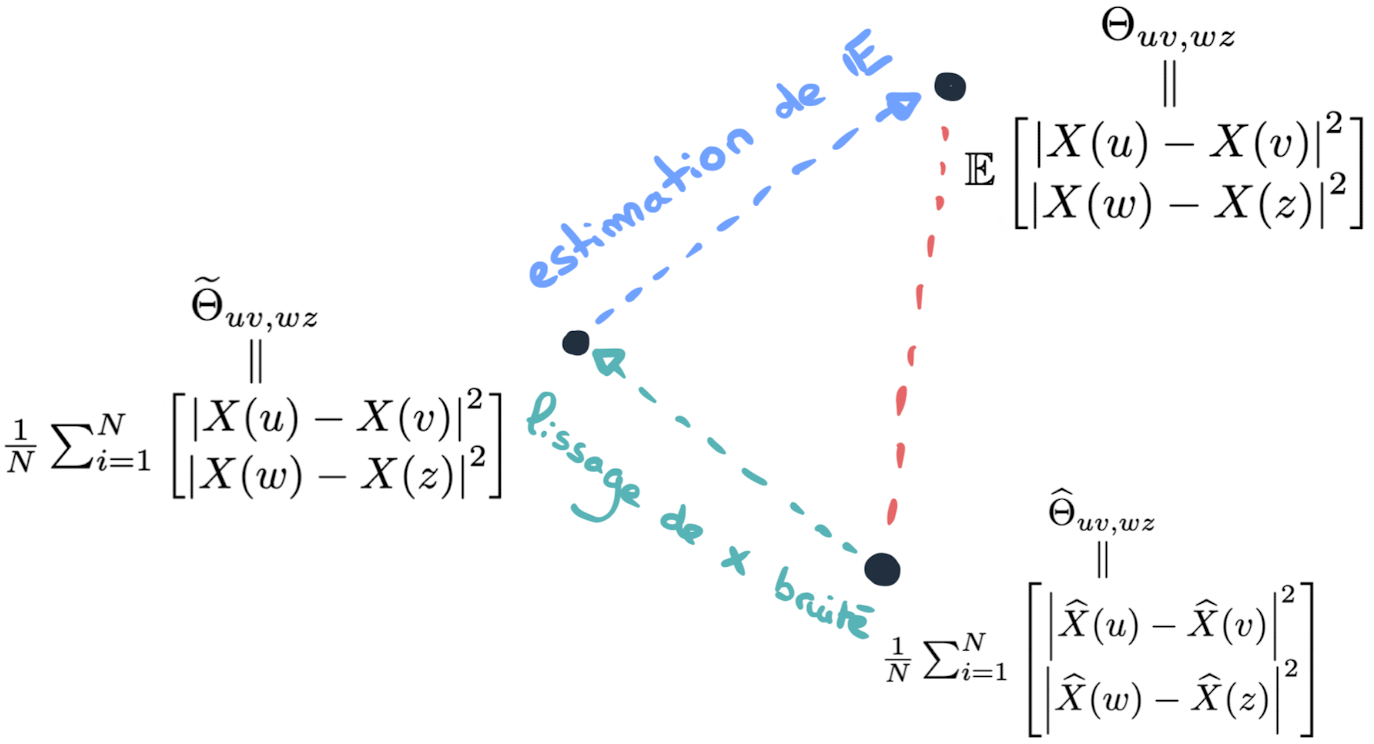
\includegraphics[width=0.7\textwidth]{Images/sketches/theta_biais.png}
	\caption{Schéma représentant les différentes approximations du couple d'incréments}
	\label{fig:sketch_theta_biais}
\end{figure}

\subsection{Choix du Risque}

\subsubsection{Distance Euclidienne}

Afin de quantifier la qualité de l'estimation conjointe du couple de $\theta$, il est raisonnable de considérer la distance euclidienne usuelle pour des vecteurs de $\R 2$

\begin{equation*}
R(\Theta, \Delta) = {\distnorme 2 {\widehat \Theta(\Delta)} {\widetilde \Theta(\Delta)}}^2
\end{equation*}

% et on nomme $R\cindexA(\Delta) = R( \thetaA , \, \Delta \, )$ et $R\cindexB(\Delta) = R( \thetaB, \, \Delta \, )$

\subsubsection{Distance Euclidienne Relative}

On va cependant considérer le risque relatif à la norme de la quantité que l'on cible :

\begin{equation*}
R(\Theta, \Delta) =\frac{ {\distnorme 2 {\widehat \Theta(\Delta)} {\widetilde \Theta(\Delta)}}^2}{ {\norme 2 {\widetilde \Theta(\Delta)}}^2 }
\end{equation*}

\question{Pourquoi considérer la distance euclidienne relative à la norme de la cible $\widetilde \Theta$ plutôt que la distance euclidienne classique qui est plus simple ?}

Le risque sert à déterminer la qualité de l'estimation du couple $\widetilde \Theta$ par $\widehat \Theta$ à un $\Delta$ donné. Il faut cependant garder à l'esprit que $\Theta$ est en réalité une fonction de $\Delta$ car la valeur de $t_1, t_2, t_3$ dépendent de $\Delta$. Ainsi la norme de $\widetilde \Theta$ va varier lorsque l'on fait varier $\Delta$\footnote{il est possible d'obtenir plus de détails en annexe \ref{annexe:tous_theta_conviennent_borne_norme_theta}}. Les risques obtenus via la norme euclidienne sont des risques qui mesurent une différence absolue, mais alors avoir un risque plus petit qu'un autre n'a pas le même sens pour différents $\Delta$ en termes de qualité d'approximation. C'est pourquoi nous considérons le risque relatif dans la détermination du critère du choix du $\Delta$.

On pourra cependant observer la différence entre le risque euclidien et le risque euclidien relatif à la norme de la cible en $\Delta$ sur les figures \ref{fig:sparse_osef} et \ref{fig:sparse_osef_rel}.

% \section{Détermination d'un critère de choix du diamètre $\Delta$ des intervalles à considérer pour l'estimation de la régularité locale}
% 
Maintenant que l'on a déterminé que l'on souhaite travailler sur un les couples $\thetaB$ et $\thetaA$, il nous faut déterminer un critère pour déterminer quel couple est plus judicieux pour la méilleure estimation en pratique des paramètres de régularité locale.

% L'heuristique est la suivante : dans les simulations, il est possible de faire 200 simulations de monte carlo et d'obtenir le $\Delta^*$ le plus proche du $\Delta$ optimal pour estimer la régularité. Dans la pratique, obtenir un tel $\Delta$ optimal n'est pas réaliste. On ne connait pas la régularité du processus que l'on souhaite estimer. L'idée est donc de favoriser le couple de $\theta(u,v)$ qui possède le plus grand plateau autour du $\Delta^*$ pour le risque euclidien \emph{si l'écart de risque enclidien entre les deux couples n'est pas trop important}. Si l'un est beaucoup plus performant que l'autre, on choisira le plus performant. Mais si la performance des deux est à peu près équivalente, autant sélectionner celui qui dans la pratique (c'est-à-dire sans avoir 200 réplications indépendantes) nous donnera le plus de flexibilité sur l'erreur commise en sélectionnant un $\Delta$ autour du $\Delta^*$ dû à la fluctuation statistique.
L'approche adoptée est la suivante : dans un contexte de simulations, il est possible de mener 200 simulations de Monte Carlo pour déterminer une valeur de $\Delta$ la plus proche du $\Delta^*$ optimal pour estimer la régularité. Cependant, dans la réalité, atteindre une valeur $\Delta$ optimale est peu probable car nous ne possédons pas d'information sur la régularité du processus que nous cherchons à estimer. Par conséquent, l'idée consiste à privilégier le couple $\theta(u,v)$ qui présente le plus grand plateau autour de $\Delta^*$ sur la base du risque euclidien, à condition que la différence de risque entre les deux couples ne soit pas trop significative. Si l'un des couples se distingue nettement en termes de performance, alors il est logique de le sélectionner. Cependant, si les performances des deux couples sont relativement similaires, il est préférable d'opter pour celui qui offre davantage de flexibilité dans la pratique (c'est-à-dire sans avoir recours à 200 réplications indépendantes) pour gérer les erreurs lors de la sélection d'un $\Delta$ autour de $\Delta^*$, compte tenu des fluctuations statistiques.

% \subsection{Détermination d'un seuil pour l'équivalence de risque quadratique}

% Il nous faut maintenant déterminer ce que l'on considère comme étant deux risques "équivalents". Pour cela on va déterminer pour différentes valeurs du véritable $H$ le seuil $\varepsilon$ sur le risque tel que $R\cindexA(\Delta + \delta) + \varepsilon$ induit une erreur d'au maximum $10$\% sur le H estimé. On viendra ensuite déterminer les $\delta$ qui en moyenne correspondent à ce seuil $\varepsilon$ pour les différentes valeurs de $H$.

% \subsection{Détermination du meilleur couple à risque \og équivalent \fg}

% A risques équivalents $R_1$ et $R_2$, on peut déterminer quel diamètre $\Delta$ recommander au praticien en sélectionnant celui qui possède le plus grand \og plateau \fg autour de l'optimum. On peut alors déterminer le diamètre à sélectionner via deux critères possibles :

% \subsubsection{en utilisant les pentes}


% La première méthode consiste à regarder les pentes à gauche et à droite du $\Delta^*$ optimal. On définit les pentes de la façon suivante :

% \begin{align*}
% 	a_g : \Delta, \delta & \mapsto \frac{R(\Delta) - R(\Delta - \delta)}{\delta} \\
% 	a_d : \Delta, \delta & \mapsto \frac{R(\Delta + \delta) - R(\Delta)}{\delta}
% \end{align*}
% On peut définir les pénalisations suivantes pour déterminer le meilleur couple à risque équivalent en terme de plateau, en pénalisant les larges différence entre la pente à gauche et à droite :

% \begin{equation*}
% 	m_q(\Delta, \delta) = \frac{a_g^2(\Delta, \delta) + a_d^2(\Delta, \delta)}{2}
% \end{equation*}

% \subsubsection{en utilisant les valeurs de risque}
% une autre méthode est de regarder directement les valeurs à gauche et à droite du $\Delta^*$ optimal. En supposant que :

% \begin{equation*}
% 	R_2(\Delta^*_2) \geq R_1(\Delta^*_1)
% \end{equation*}

% \begin{equation*}	
% 	dR = \bigl\vert R_1(\Delta^*_1) - R_2(\Delta^*_2) \bigr\vert
% \end{equation*}

% on compare désormais les valeurs recentrées :

% \begin{align*}
% 	r_g^{[2]} & = R_2(\Delta^*_2 - \delta) - dR \\
% 	r_d^{[2]} & = R_2(\Delta^*_2 + \delta) - dR
% \end{align*}

% aux valeurs du risque sur la courbe correspondant à l'autre couple d'incréments :

% \begin{align*}
% 	r_g^{[1]} & = R_1(\Delta^*_1 - \delta) \\
% 	r_d^{[1]} & = R_1(\Delta^*_1 + \delta)
% \end{align*}

% avec le critère de sélection suivant :

% % \begin{equation*}
% % 	\argmin \bigl( \frac{r_g^{[1]} + r_d^{[1]}}{2}, \frac{r_g^{[2]} + r_d^{[2]}}{2}  \bigr)
% % \end{equation*}
% \idee{Pour pénaliser les solutions où la pente à gauche est très différente de la pente à droite en magnitude, on peut considérer d'élever $r_g$ et $r_d$ au carré.}

% \begin{equation*}
% 	\argmin\limits_{[1] \textsf{ ou } [2]} \bigl( \frac{(r_g^{[1]})^2 + (r_d^{[1]})^2}{2}, \frac{(r_g^{[2]})^2 + (r_d^{[2]})^2}{2}  \bigr)
% \end{equation*}


\subsubsection{résultat et détermination de la procédure de sélection du $\Delta$}
\label{sec:proc_delta}

\warn{
	Il est important de garder en tête le modèle dans lequel on s'est placé pour étudier le comportement du $\Delta$. La recommendation qui est faite pour la sélection du $\Delta$ est valable pour :

	\begin{itemize}
		\item $\operatorname{FAR}(1)$ construit à partir d'un $\operatorname{mfBm}(H, L)$
		\item la régularité donnée par $H(t)$, qui dans notre cas est $\mathcal C^\infty$ sur $[0,1]$
		\item le noyau de la relation auto-régressive $\beta$ est une fonction de classe $\mathcal C^{\infty}$ sur $]0, 1]$ et continue en $0$
		\item La dérivée de $H$ est $H' :t \mapsto \frac{2 e ^{-5(t-0.5)}}{\left(1 + e ^{-5(t-0.5)}\right)^2}$, la variation maximale de la régularité est atteinte en $\argmax\limits_{t \in [0,1]} H'(t) = \frac 1 2$ avec $H'(\frac 1 2)=\frac 1 2$
		\item La régularité est monotone et strictement croissante sur $[0,1]$
	\end{itemize}

	Trop s'éloigner de ces hypothèses pourrait demander d'analyser de nouveau le comportement du $\Delta$ dû aux propriétés de certaines de ces quantités qui aurrait pu influencer le résultat.
}

\question{Quelle procédure est recommandée pour la sélectionner un $\Delta$ adapté pour l'estimation de la régularité locale ?}

On va distinguer 2 cas : 
\begin{enumerate}
	\item Le lissage des courbes a été effectué avec une fenêtre de lissage individuelle, sélectionnée par validation croisée sur chaque courbe : méthode optimale.
	\item Le lissage des courbes a été effectué avec une fenêtre de lissage globale, sélectionnée via la médiane des fenêtres de lissage sur les premières courbes déterminées par validation croisée\footnote{Notons qu'il ne faut pas sélectionner des courbes aléatoirement mais plutôt les premières courbes car les données ont de la dépendance.} : économie de calcul.
\end{enumerate}


\begin{itemize}
	\item \textbf{lissage individuel} :
	\begin{enumerate}
		\item 
	\end{enumerate}
	\item \textbf{lissage global} :
	\begin{enumerate}
		\item 
	\end{enumerate}
\end{itemize}



\section{Récapitulatif de la qualité des estimations pour la stratégie de \og lissage global \fg}
Les simulations de Monte Carlo permettent d'avoir accès directement à la véritable régularité de la courbe en chaque point. Nous allons dans l'étude du comportement du $\Delta$ essayer de tirer profit de cet avantage que ne possède pas le praticien qui utilise des données réelles.

\warn{On rappelle que la stratégie de lissage dite \of globale \fg lisse par validation croisée courbe par courbe pour $\lambda < 110$ puis calcule une fenêtre de lissage médiane à appliquer sur toutes les courbes pour $\lambda > 110$}

\subsection{Récapitulatif concernant le risque quadratique sur l'estimation de la régularité}

\begin{table}[H]
    \centering
    \begin{tabular}{l|ll|}
        \cline{2-3}
                                              & $\lambda < 120$                                                                                                                                                                                                    & $\lambda \geq 120$                                                                                                                                        \\ \hline
        \multicolumn{1}{|l|}{$H_t \leq 0.65$} & \multicolumn{1}{l|}{\begin{tabular}[c]{@{}l@{}}$\yesequiv \mathcal R$\\ $\yesequiv \Delta^*$\\ $\Delta^- \downarrow 0.01$\end{tabular}}                                                                            & \begin{tabular}[c]{@{}l@{}}$\simeq \yesequiv \mathcal R$\\ $\notequiv \Delta^*$\\ $\Delta^+ \rightarrow [\leq 0.6] 0.1/0.2 [\geq 0.6]$\end{tabular}        \\ \cline{2-3}
        \multicolumn{1}{|l|}{$H_t > 0.65$}    & \multicolumn{1}{l|}{\begin{tabular}[c]{@{}l@{}}$\yesequiv \mathcal R$\\ $\notequiv \Delta^*$\\ \faExclamationTriangle $H=0.7 : \Delta^- = 0.02$\\ \faExclamationTriangle $H = 0.73 : \Delta^- = 0.2$\end{tabular}} & \begin{tabular}[c]{@{}l@{}}$\thetaA$\\ \faExclamationTriangle $H=0.7 : \Delta^+ = 0.02$\\ \faExclamationTriangle $H = 0.73 : \Delta^+ = 0.2$\end{tabular} \\ \hline
    \end{tabular}
    \caption{Tableau récapitulatif des $\Delta$ optimaux : Risque sur $H_t$}
    \label{tab:recap_delta_H}
\end{table}

\subsection{Récapitulatif concernant le risque quadratique sur les $\theta$ individuellement}

\begin{table}[H]
	\centering
	\begin{tabular}{l|ll|}
		\cline{2-3}
		                                     & $\lambda < 120$                                                                                                       & $\lambda \geq 120$                                                                            \\ \hline
		\multicolumn{1}{|l|}{$H_t < 0.6$}    & \multicolumn{1}{l|}{\begin{tabular}[c]{@{}l@{}}meilleur : $\thetaC$\\ \\ \\ $\Delta^- \rightarrow 0.01$\end{tabular}} & \begin{tabular}[c]{@{}l@{}}meilleur : $\thetaA$\\ \\ $\Delta^+ \rightarrow 0.2$\end{tabular}  \\ \cline{2-3}
		\multicolumn{1}{|l|}{$H_t \geq 0.6$} & \multicolumn{1}{l|}{\begin{tabular}[c]{@{}l@{}}meilleur : $\thetaA$\\ \\ $\Delta^- \rightarrow 0.2$\end{tabular}}     & \begin{tabular}[c]{@{}l@{}}meilleur : $\thetaC$\\ \\ $\Delta^+ \rightarrow 0.01$\end{tabular} \\ \hline
	\end{tabular}
	\caption{Tableau récapitulatif des $\Theta$ optimaux : Risque individuel sur $\tilde \theta(u,v)$}
	\label{tab:recap_theta_single}
\end{table}



\subsection{Récapitulatif concernant le risque euclidien pour les couple $\Theta$}

\begin{table}[H]
	\centering
	\begin{tabular}{l|ll|}
		\cline{2-3}
		                                     & $\lambda < 120$                                                                                                                                                                                                           & $\lambda \geq 120$                                                                             \\ \hline
\multicolumn{1}{|l|}{$H_t < 0.6$}    & \multicolumn{1}{l|}{\begin{tabular}[c]{@{}l@{}}$\yesequiv \mathcal R, \Delta^*$\\ $\Delta^*_- = 0.01$\end{tabular}}                                                                                                       & \begin{tabular}[c]{@{}l@{}}meilleur : $\thetaB$\\ $\Delta^*_+ = 0.2$\end{tabular}                         \\ \cline{2-3}
\multicolumn{1}{|l|}{$H_t \geq 0.6$} & \multicolumn{1}{l|}{\begin{tabular}[c]{@{}l@{}}meilleur : $\thetaB$\\ $\Delta^*_- = 0.2$\\ \\\faExclamationTriangle $H=0.7 : \Delta^- = 0.01 \oplus \yesequiv \mathcal R$\\ \\\faExclamationTriangle $H=0.8 : \thetaA$\end{tabular}} & \begin{tabular}[c]{@{}l@{}}$\yesequiv \mathcal R, \Delta^*$\\ $\Delta^*_+ = 0.01$\end{tabular} \\ \hline
	\end{tabular}
	\label{tab:recap_delta_eucl_h_global_pour_lambda_sup}
	\caption{Tableau récapitulatif des $\Delta$ optimaux : Risque euclidien sur $\tilde \Theta$ | fenêtre de prélissage globale pour $\lambda \geq 120$}
\end{table}

\subsection{Conclusion des tables}

Le risque euclidien a une structure plus complexe que le risque relatif sur la détermination du $\Delta$ optimal\footnote{$cf$ différence entre les  graphes \ref{fig:sparse_osef} (euclidien) et \ref{fig:sparse_osef_rel} (relatif)}. Concernant le risque euclidien, on peut recommander, en s'appuyant conjointement sur les observations graphiques ayant enlevé les observations extrêmes (figures \ref{fig:compare_xtrm_2} et \ref{fig:sparse_osef})

\section{Etude de l'impact de la méthode de sélection de la fenêtre de pré-lissage sur le risque d'estimation des couples $\Theta$}

\subsection{Rappel de la méthodologie utilisée}

Afin de simplifier les notations, dans la suite nous nous référons à 2 cas de méthodologie différentes nommées \og \textbf{individuel} \fg et \og \textbf{global} \fg. Cependant le nom choisi ne reflète pas entièrement la procédure, il faut donc bien garder en tête ce qu'on attend par ces noms de méthodologie :

\begin{table}[H]
	\centering
	\begin{tabularx}{\textwidth}{c|X|X}
		\toprule
		threshold/méthodologie & \textbf{individuel}                  & \textbf{global}                                                                                                                                                                                                               \\
		\bottomrule
		\\
		$\lambda < 110$        & $h$ cross-validé \textbf{par courbe} & $h$ cross-validé \textbf{par courbe}
		\\
		\midrule
		\\
		$\lambda \geq 100$     & $h$ cross-validé \textbf{par courbe} & détermination de 50 fenêtres $h_i$ cross-validées sur les 50 premières courbes puis utilise $h = \operatornamewithlimits{med}\limits_{i \in \llbracket 1, 50 \rrbracket} h_i^{*-\textsf{cv}}$ sur \textbf{toutes les courbes}
		\\
		\bottomrule
	\end{tabularx}
\end{table}

Ce rappel sera important dès la prochaine section portant sur le comportement du cas sparse.

\subsection{Le cas sparse}

les tables \ref{tab:couple_1312_indiv_vs_glob} et \ref{tab:couple_1323_indiv_vs_glob} indiquent que la différence en terme de performance sur le Risque entre un lissage global (déterminé comme la médiane des fenêtres cross-validées sur les 50 premières courbes) et un lissage individuel (la fenêtre de lissage de chaque courbe est déterminée par validation croisée) devient mineure une fois que le nombre moyen de points par courbe devient \og dense \fg. Dans notre cas, on voit qu'à partir de $\lambda = 150$, la différence entre la médiane du risque par lissage à fenêtre globale et par lissage individuel devient faible (de l'ordre de $10^{-6}$ à $10^{-3}$) et une différence de variance presque imperceptible (de l'ordre de $10^{-9}$ à $10^{-5}$).




\warn{A la vue de ces résultats il semblerait que la conclusion évidente soit de faire une fenêtre cross-validée individuelle lorsque l'on est dans un cas sparse. Sauf qu'il ne faut pas oublier que dans l'appellation \og global \fg comme mentionné précédemment, les différentes courbes étaient déjà lissées individuellement lorsque $\lambda < 110$.}

\question{D'où viennent alors de telles différences ?}

Un changement d'algorithme a été opéré entre les lissages effectués avec la méthode \og globale \fg (première méthode utilisée) et la méthode \og individuelle \fg : lorsqu'il existe un endroit où on lisse pour déterminer la régularité tel qu'il n'y a pas assez de points autour, on ne sélectionne pas la fenêtre associée.

Sous R, entre autre, l'implémentatione st telle que si le lissage à noyau renvoie \mintinline{R}{NaN}, on ne choisit pas le $h$ associé :


\begin{minted}[linenos=true, mathescape=false, frame=single, breaklines]{R}
cv_error <- sapply(h_grid, function(hi, y, t, K) {
	yhat <- estimate_nw(y = y, t = t, h = hi, tnew = t, smooth_ker = K)$yhat
	wmat <- outer(X = t, Y = t, function(u, v) K((u - v) / hi))
	metric <- (y - yhat) / (1 - K(0) / rowSums(wmat))

	# If there is only one value in the kernel support, it return NaN.
	error_hi <- mean(metric[!is.nan(metric)]**2)
}, y = y, t = t, K = smooth_ker)

# If cv_error is NaN, do take it into account
if (any(is.nan(cv_error))) {
	h_grid <- h_grid[-which(is.nan(cv_error))]
	cv_error <- cv_error[!is.nan(cv_error)]
	hcv <- h_grid[which.min(cv_error)]
}
\end{minted}

\chk{$\circled 1$ Il semblerait donc que cette différence de traîtement du nombre de points autour des points lissés soit ce qui explique la différence entre les deux méthodes pour le cas sparse, ce qui semble raisonnable : on ne voit pas de différence dans le cas dense simplement car ne pas avoir suffisamment de points autour se rarifie extrêment.
}

\chk{
	$\circled 2$ On notera tout de même que la faible différence de médiane et de variance entre le cas \og global \fg et \og individuel \fg indique qu'il est possible d'économiser en temps de calcul sur des données même corrélées en calculant une fenêtre globale à partir des premières courbes lorsque l'on dispose d'observations denses à moindre coût sur le risque.
}

\subsection{Densité de points sur les courbes observées}

\subsubsection{Densité moyenne}

Les figures \ref{fig:den_ex} et \ref{fig:den_counterex} affichent la densité de points présents autour de $t_2 = 0.8$ en considérant toutes les courbes pour un individu de monte-carlo associé à un risque extrême. En utilisant un estimateur de Parzen-Rosenblatt de fenêtre $\Delta$ utilisé pour calculer $X\bigl( \, t_1(\Delta) \, \bigr)$ et $X\bigl( \, t_3(\Delta) \, \bigr)$ :

\begin{equation*}
	\widehat f_T = \frac 1 N \sum\limits_{i=1}^N \frac 1 {M_i} \sum\limits_{m=1}^{M_i} \frac 1 \Delta K\left( \frac{t - T_i[\, m \, ]}{\Delta} \right)
\end{equation*}

De ces figures on peut déduire les conclusions suivantes : il semblerait que l'affichage de la densité de points autour du point problématique indique que les valeurs de risque extrêmes interviennent lorsqu'il existe peu ou pas de points sur l'ensemble des courbes en $t_1$ ou $t_3$. Toutefois, on pourra fournir en contre-exemple la figure \ref{fig:den_counterex}, qui indique dans un rayon $\Delta$ une densité constante de points (ce qui est en accord avec une simulation uniforme de points sur $\mathcal T$ lorsque le nombre moyen de points par courbe devient relativement dense : $\lambda = 210$).



\subsection{Peut-on considérer que tous les $\Delta$ conviennent ?}

Nous observons sur les différents graphes des risques de l'ordre de grandeur de $10^{-2}$ ou même de $10^{-3}$. La question que l'on se pose désormais est si il est raisonnable de penser que ne pas choisir le $\Delta^*$ optimal n'est pas si important dans l'estimation du couple $\Theta$.

Ce que nous allons observer est qu'il est tout de même préférable de bien déterminer le $\Delta$

\begin{equation}
	\theta(u,v) = \esperanceloi X { \bigl| X(v) - X(u) \bigr|^2 } \leq L_{J(\Delta)}^2 \bigl| v - u \bigr|^{2 H_{J(\Delta)}}
\end{equation}

sachant que l'on évalue :

\begin{equation}
	\textsf{soit }
	\thetaA = \begin{bmatrix} \theta(t_1, t_3) \\ \theta(t_1, t_2) \end{bmatrix}
\end{equation}
\begin{equation}
	\textsf{soit }
	\thetaB = \begin{bmatrix} \theta(t_1, t_3) \\ \theta(t_2, t_3) \end{bmatrix}
\end{equation}


avec :

\begin{equation}
	\begin{array}{ccc}
		|t_3 - t_1| & = \Delta
		\\
		|t_3 - t_2| & = \frac \Delta 2 & = |t_2 - t_1|
	\end{array}
\end{equation}

et donc :

\begin{equation}
	\displaystyle
	\begin{array}{rclr}
		\norme 2 \Theta & =    & \sqrt{\theta_{13}^{\,2} + \theta_{12/23}^{\, 2}}
		\\
		                & \leq & \sqrt{ L_{J(\Delta)}^4 \bigl( \, \Delta^{4 H_{J(\Delta)}} \left[ 1 + \frac 1 2 \right]  \, \bigr) }
		\\
		                & =    & L_{J(\Delta)}^2 \cdot \Delta^{2H_{J(\Delta)}} \cdot \sqrt{\frac 3 2}
	\end{array}
\end{equation}

Et donc :

\begin{equation*}
	\norme 2 \Theta \leq L_{J(\Delta)}^2 \cdot \Delta^{2H_{J(\Delta)}} \cdot \sqrt{\frac 3 2}
\end{equation*}

En utilisant les données de la simulation, $L = 1$, on obtient :

\begin{equation}
	\begin{array}{ccc}
		H_{J(\Delta)} = 0.4  & \implies & \norme 2 \Theta
		\begin{cases}
			\lesssim 3 \cdot 10^{-2} \quad & \Delta = 0.01
			\\
			\lesssim 3\cdot 10^{-1} \quad  & \Delta = 0.2
		\end{cases}
		\\\\
		H_{J(\Delta)} = 0.5  & \implies & \norme 2 \Theta
		\begin{cases}
			\lesssim 1 \cdot 10^{-2} \quad & \Delta = 0.01
			\\
			\lesssim 2\cdot 10^{-1} \quad  & \Delta = 0.2
		\end{cases}
		\\\\
		H_{J(\Delta)} = 0.6  & \implies & \norme 2 \Theta
		\begin{cases}
			\lesssim 5 \cdot 10^{-3} \quad & \Delta = 0.01
			\\
			\lesssim 2\cdot 10^{-1} \quad  & \Delta = 0.2
		\end{cases}
		\\\\
		H_{J(\Delta)} = 0.73 & \implies & \norme 2 \Theta
		\begin{cases}
			\lesssim 1 \cdot 10^{-3} \quad & \Delta = 0.01
			\\
			\lesssim 1\cdot 10^{-1} \quad  & \Delta = 0.2
		\end{cases}
	\end{array}
\end{equation}

Ainsi, la différence de risque entre l'optimum et le pire cas étant de l'odre de $10^{-2}$ dans un cas très sparse comme dans la figure \ref{fig:sparse_osef} et dans un cas raisonnablement dense on observe même des différences de l'ordre de $10^{-3}$ pour le plus régulier.


\begin{table}[H]
	\centering
	\begin{tabularx}{0.7\textwidth}{|cc|X|X|}
		\toprule
		\textbf{H} & $\mathbf{\lambda}$ & \textbf{Différence : } $\mathbf{\mathcal R_{max} - \mathcal R_{min}}$ & ordre de gradeur de la borne de $\norme 2 \Theta$ \\
		\midrule
		0.51       & 60                 & 3.3 $\cdot 10^{-2}$                                                   & $\Delta^* \simeq 0.2$ : $10^{-1}$                 \\
		0.51       & 210                & 1.1 $\cdot 10^{-2}$                                                   & $\Delta^* \simeq 0.2$ : $10^{-1}$                 \\
		\midrule
		0.6        & 60                 & 4.2 $\cdot 10^{-2}$                                                   & $\Delta^* \simeq 0.01$ : $10^{-3}$                 \\
0.6        & 210                & 1.2 $\cdot 10^{-2}$                                                   & $\Delta^* \simeq 0.01$ : $10^{-3}$                 \\
		\midrule
0.73       & 60                 & 1.2 $\cdot 10^{-2}$                                                   & $\Delta^* \simeq 0.01$ : $10^{-3}$                 \\
0.73       & 210                & 5.4 $\cdot 10^{-3}$                                                   & $\Delta^* \simeq 0.01$ : $10^{-3}$                 \\
		\bottomrule
	\end{tabularx}
\end{table}


\begin{figure}[H]
	\centering
	\textbf{ H = 0.51 }

	Sparse :

	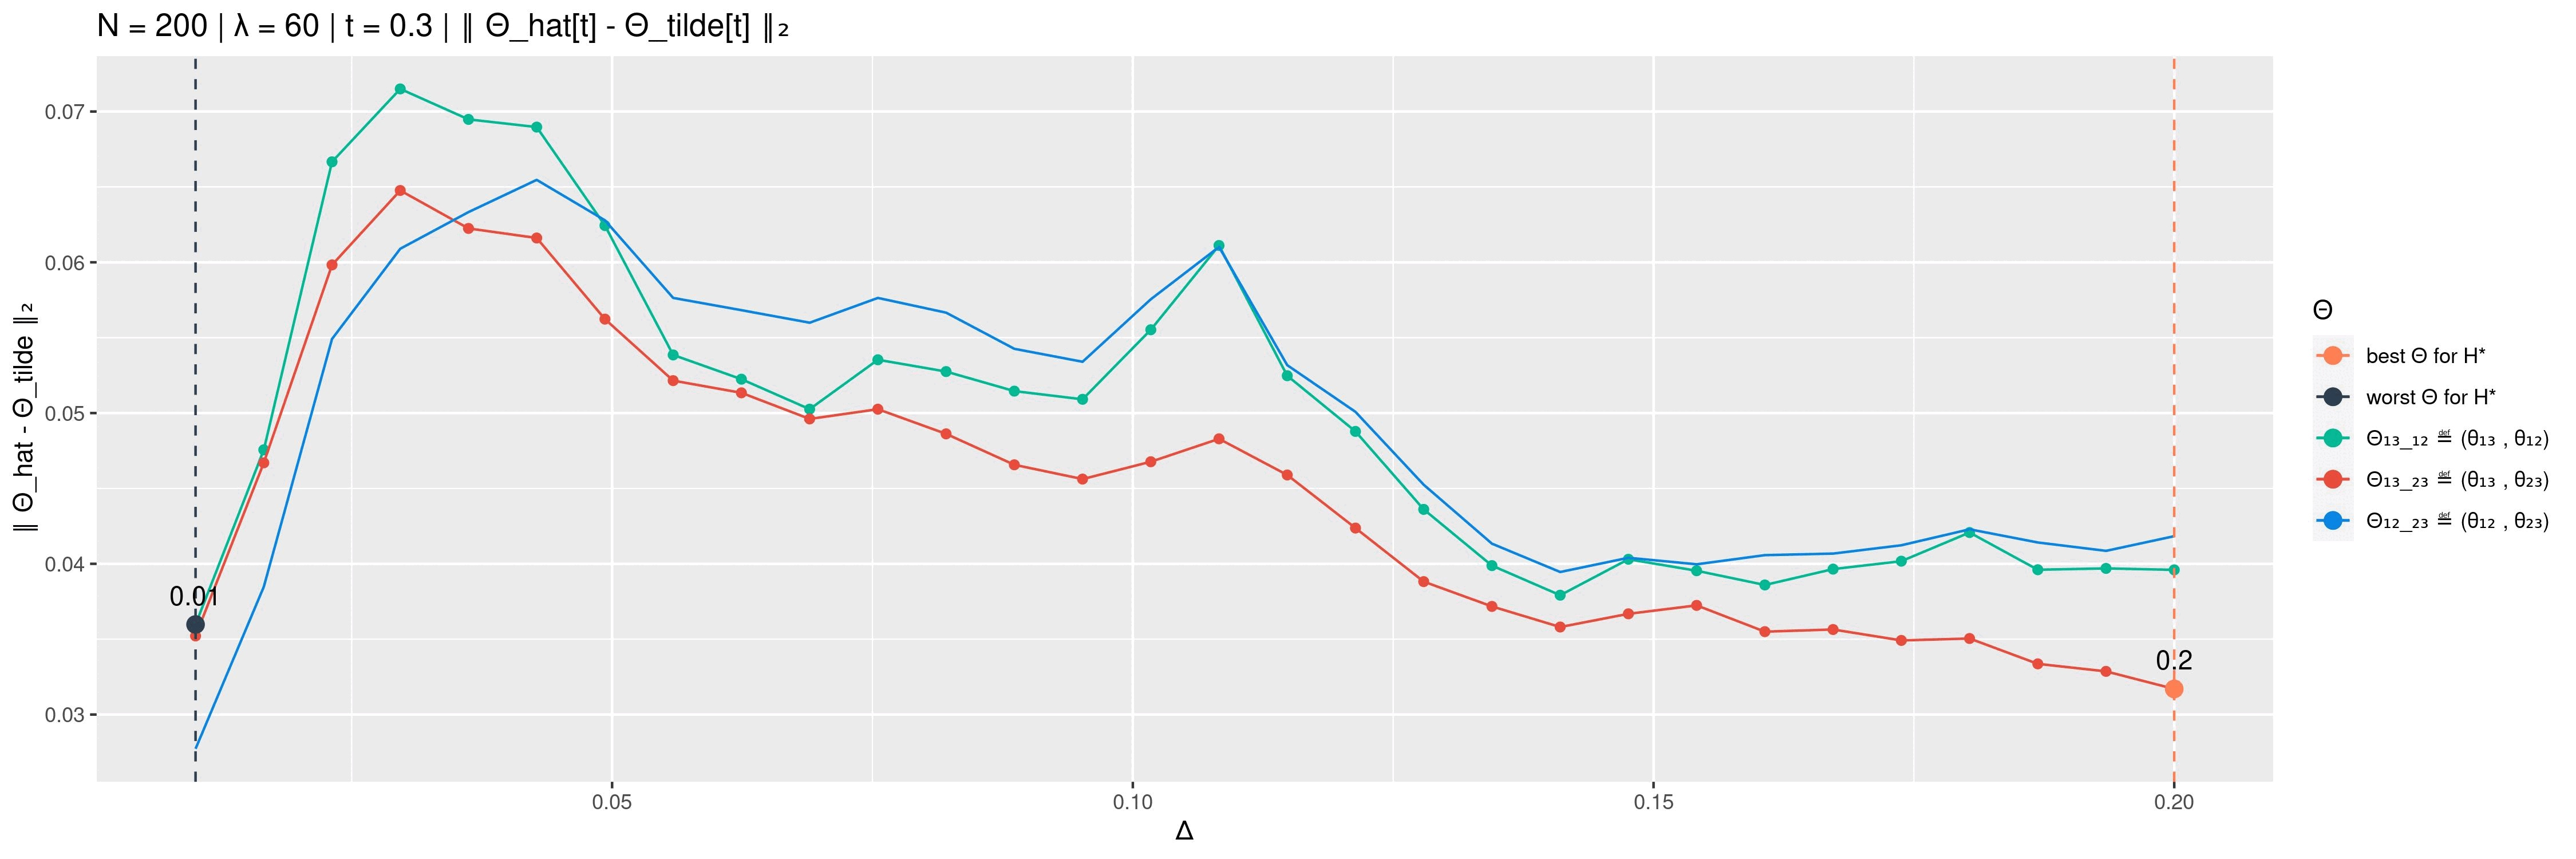
\includegraphics[width=0.8\textwidth]{Images/risque/N200_t0.3_lbd60.jpg}

	Dense :

	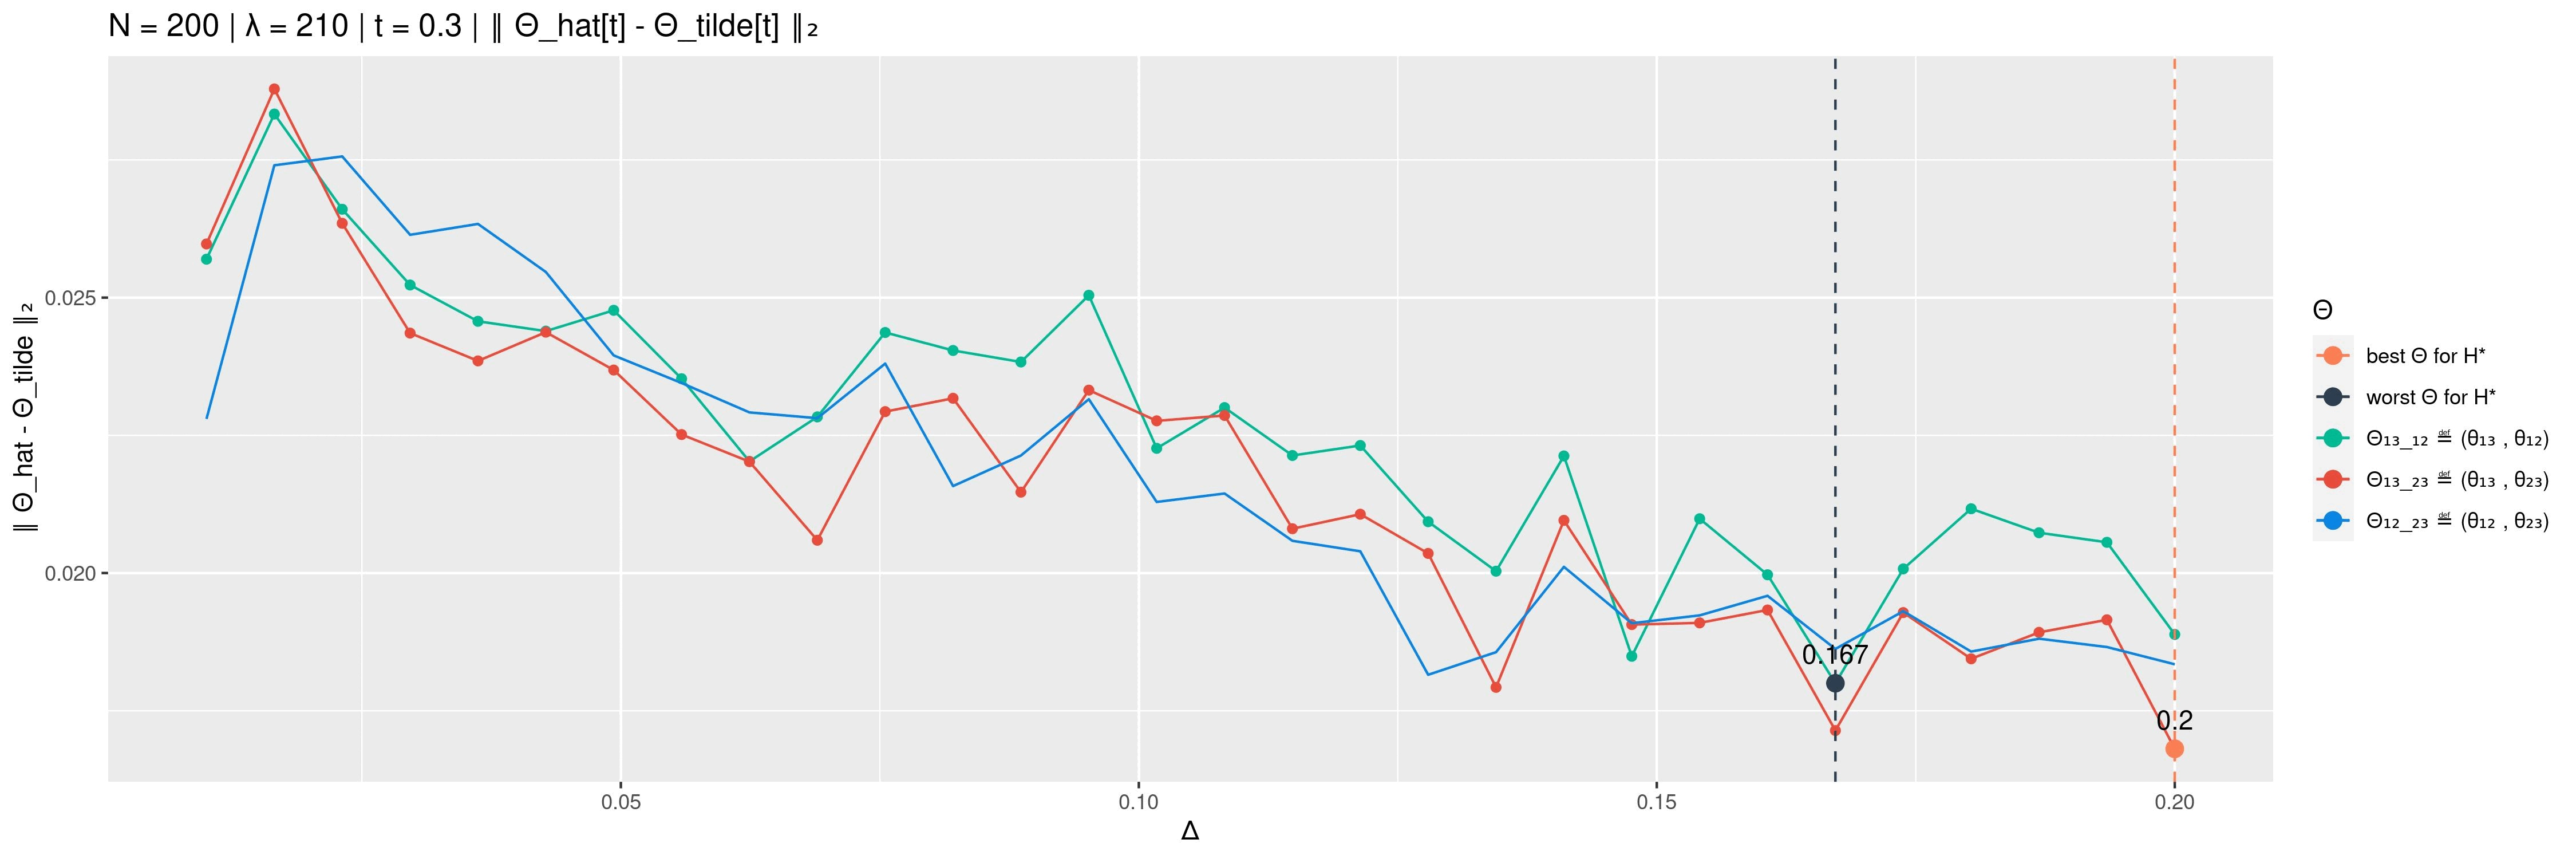
\includegraphics[width=0.8\textwidth]{Images/risque/N200_t0.3_lbd210.jpg}
\end{figure}

\begin{figure}[H]
	\centering
	\textbf{ H = 0.6 }

	Sparse :

	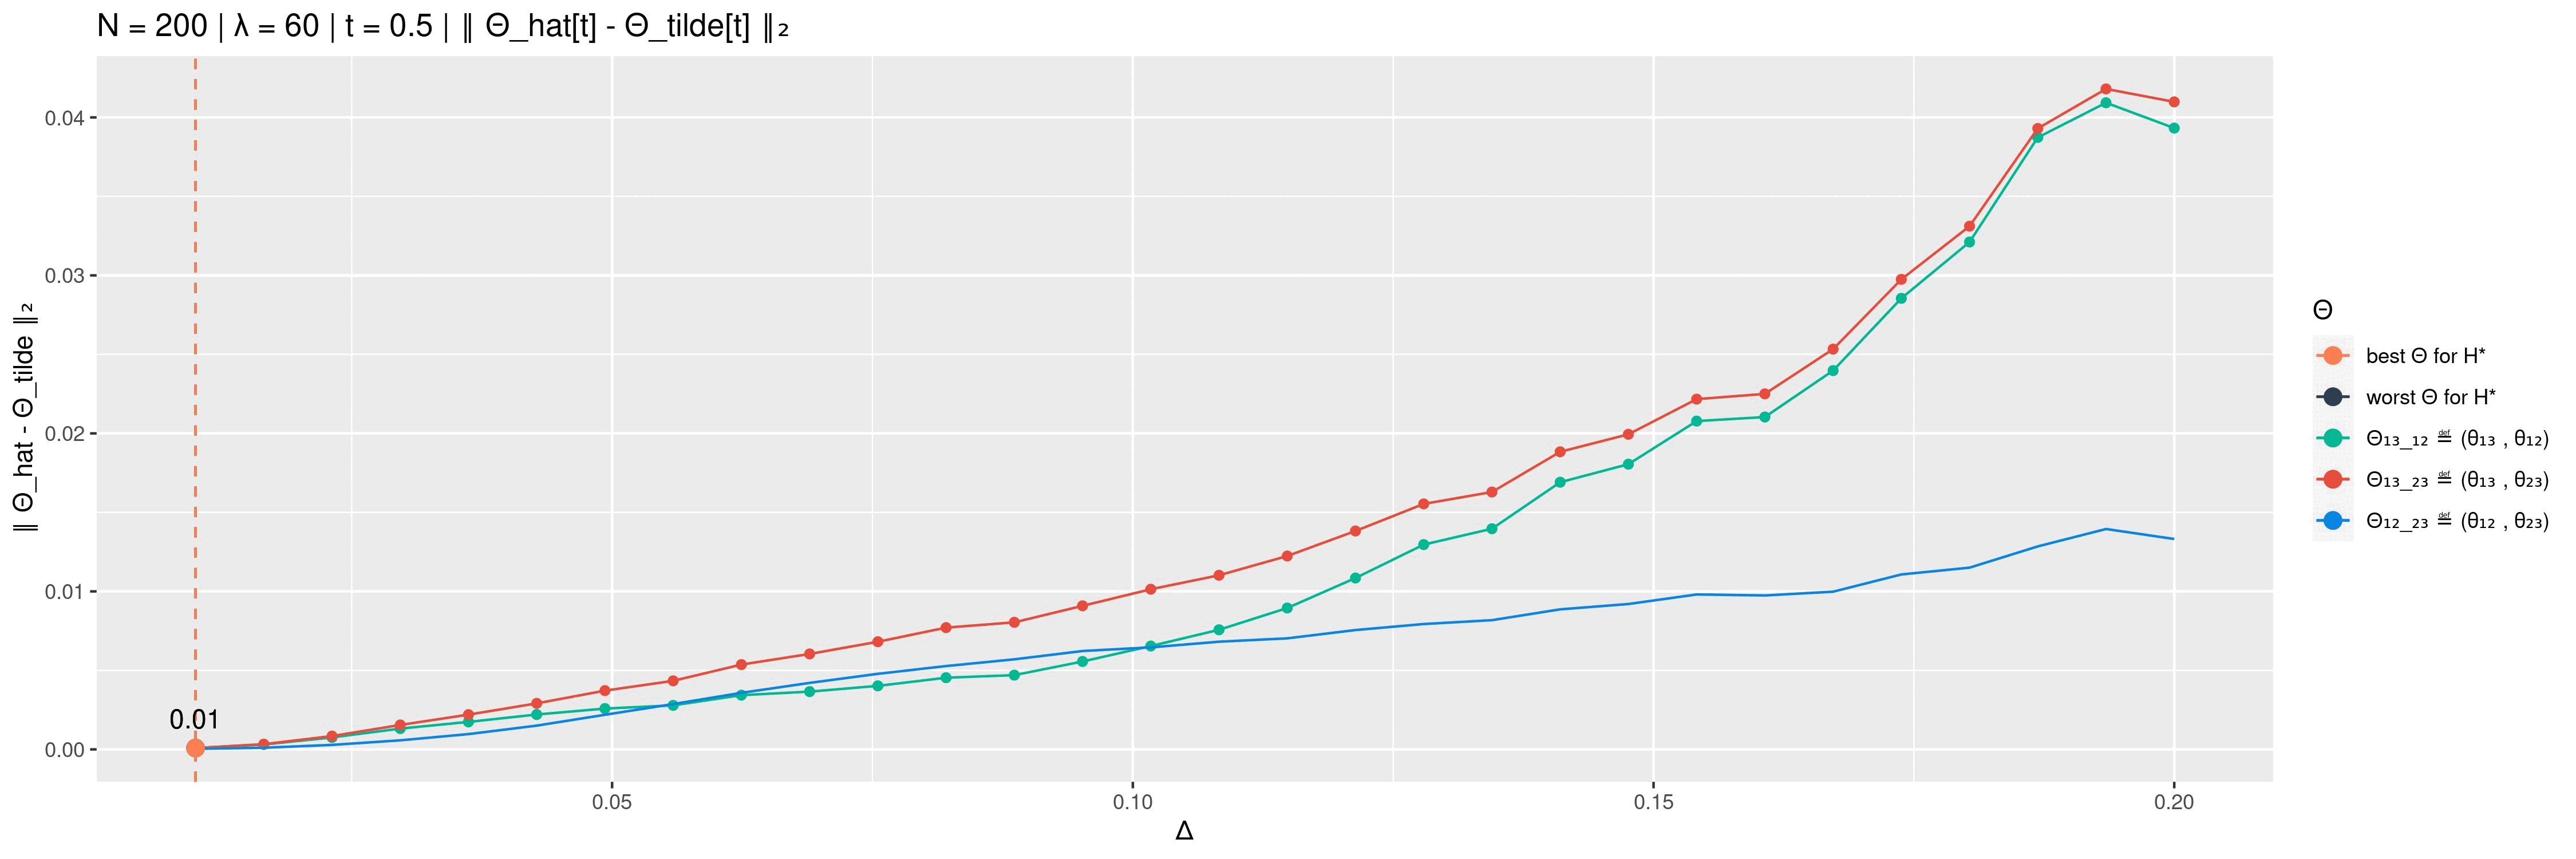
\includegraphics[width=0.8\textwidth]{Images/risque/N200_t0.5_lbd60.jpg}

	Dense :

	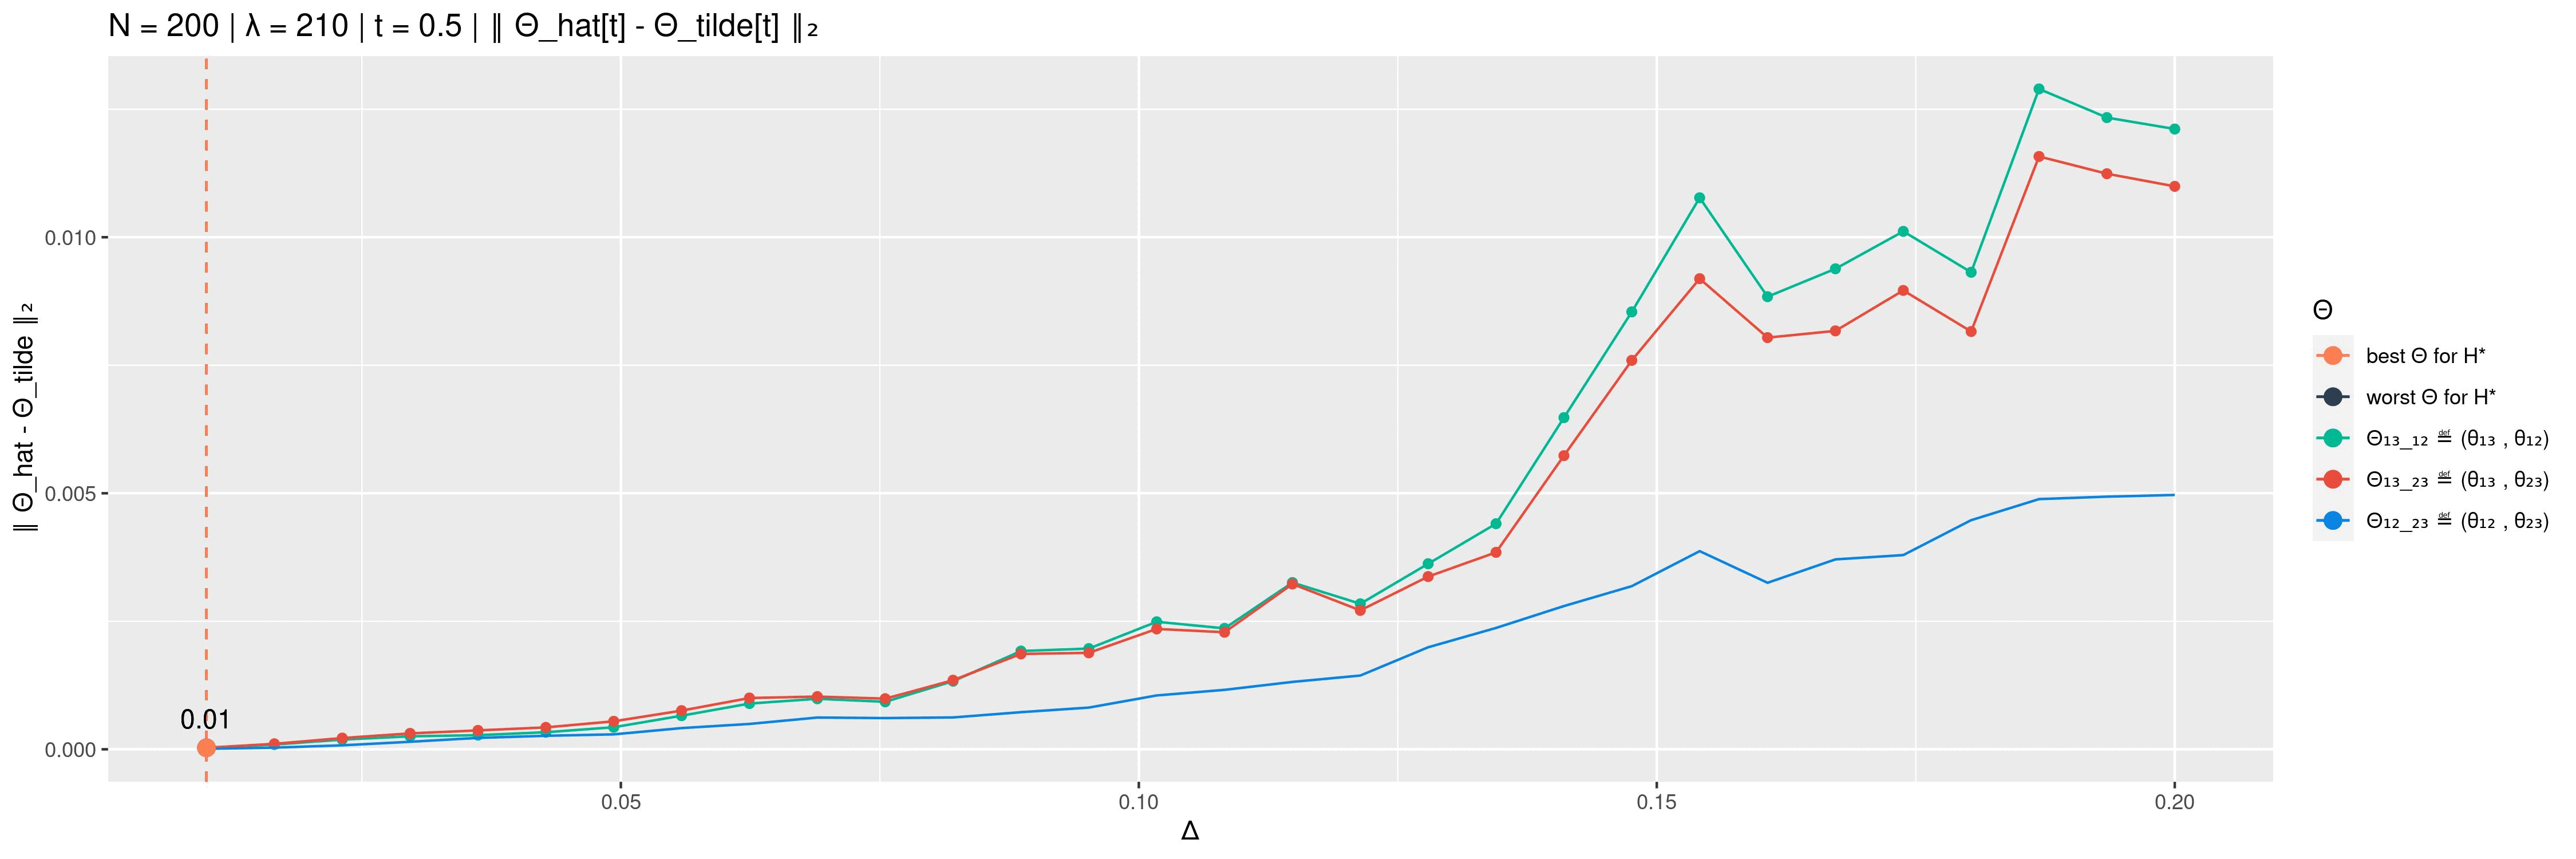
\includegraphics[width=0.8\textwidth]{Images/risque/N200_t0.5_lbd210.jpg}
\end{figure}


\begin{figure}[H]
	\centering
	\textbf{ H = 0.73 }

	Sparse :

	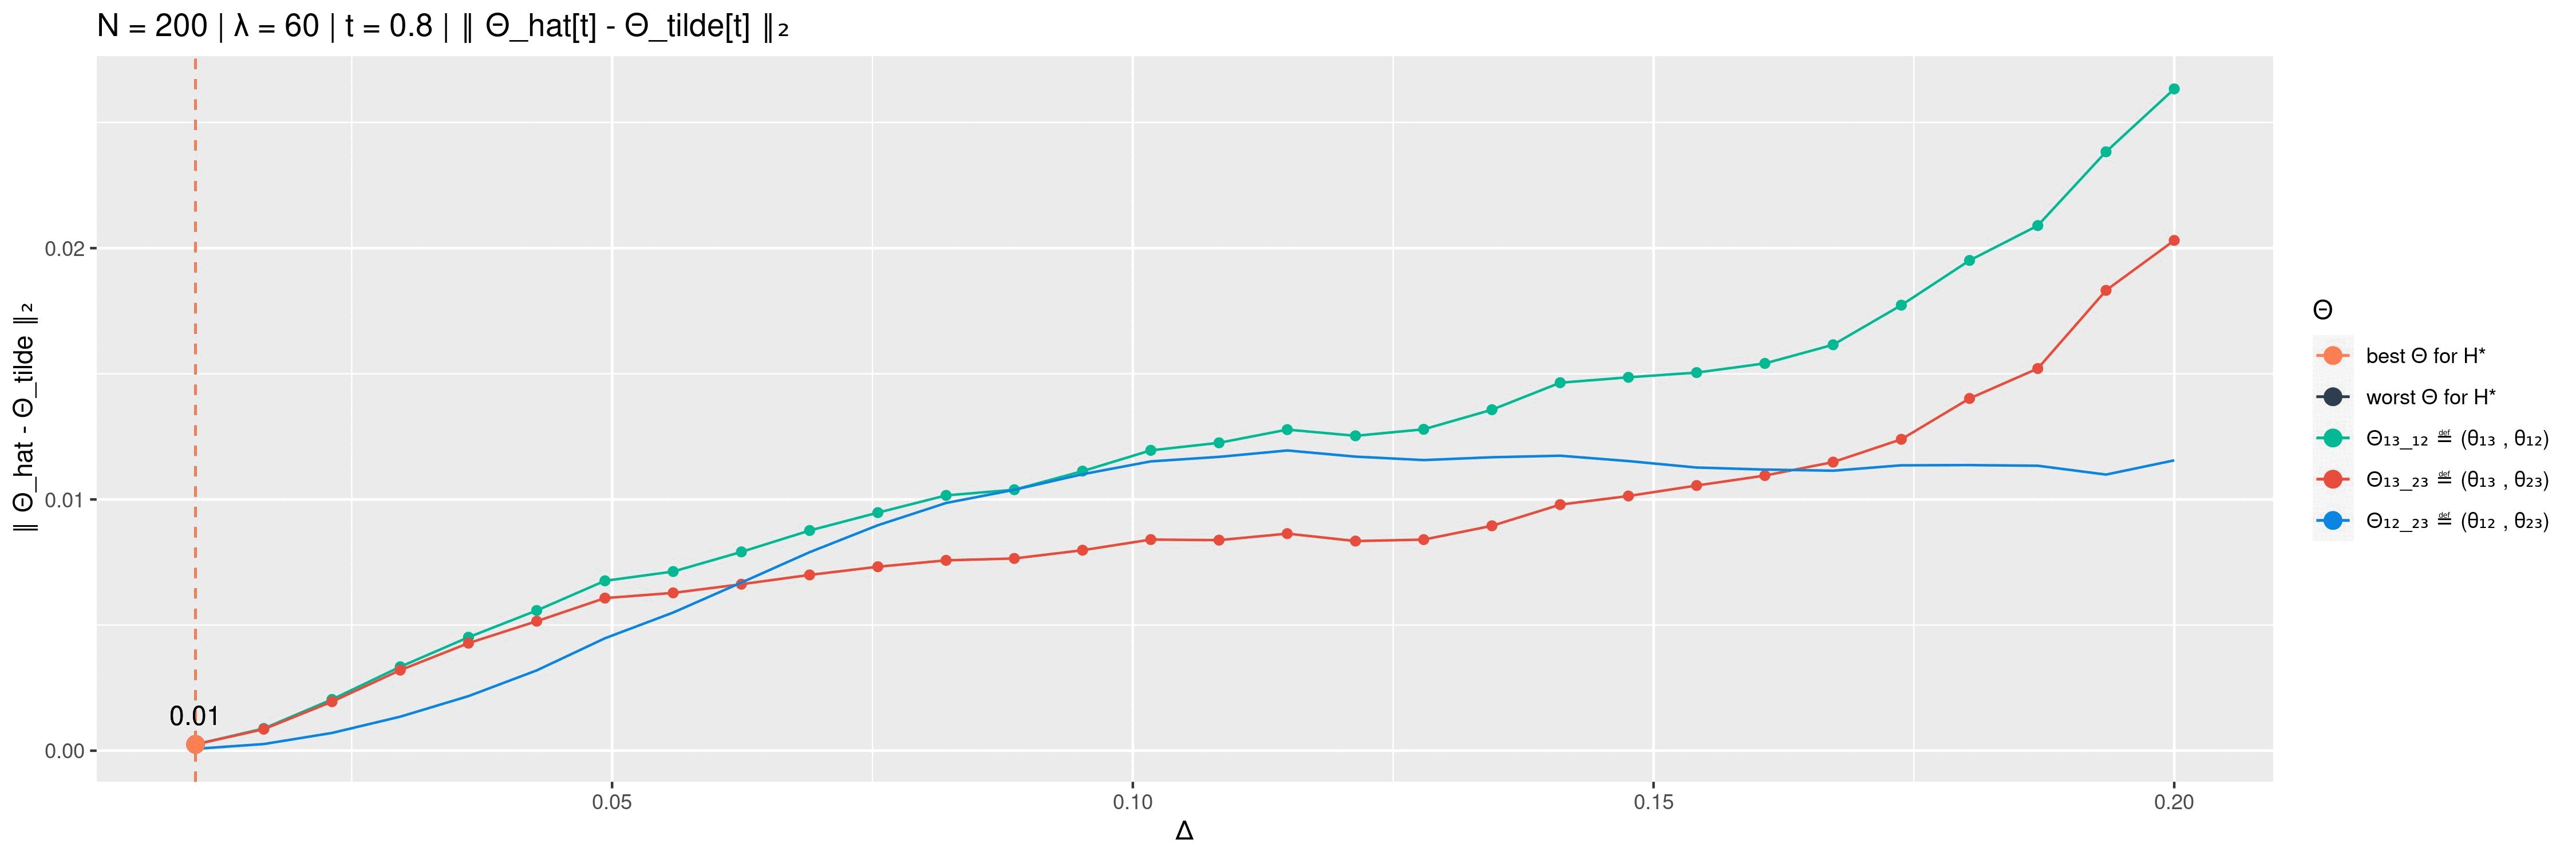
\includegraphics[width=0.8\textwidth]{Images/risque/N200_t0.8_lbd60.jpg}

	Dense :

	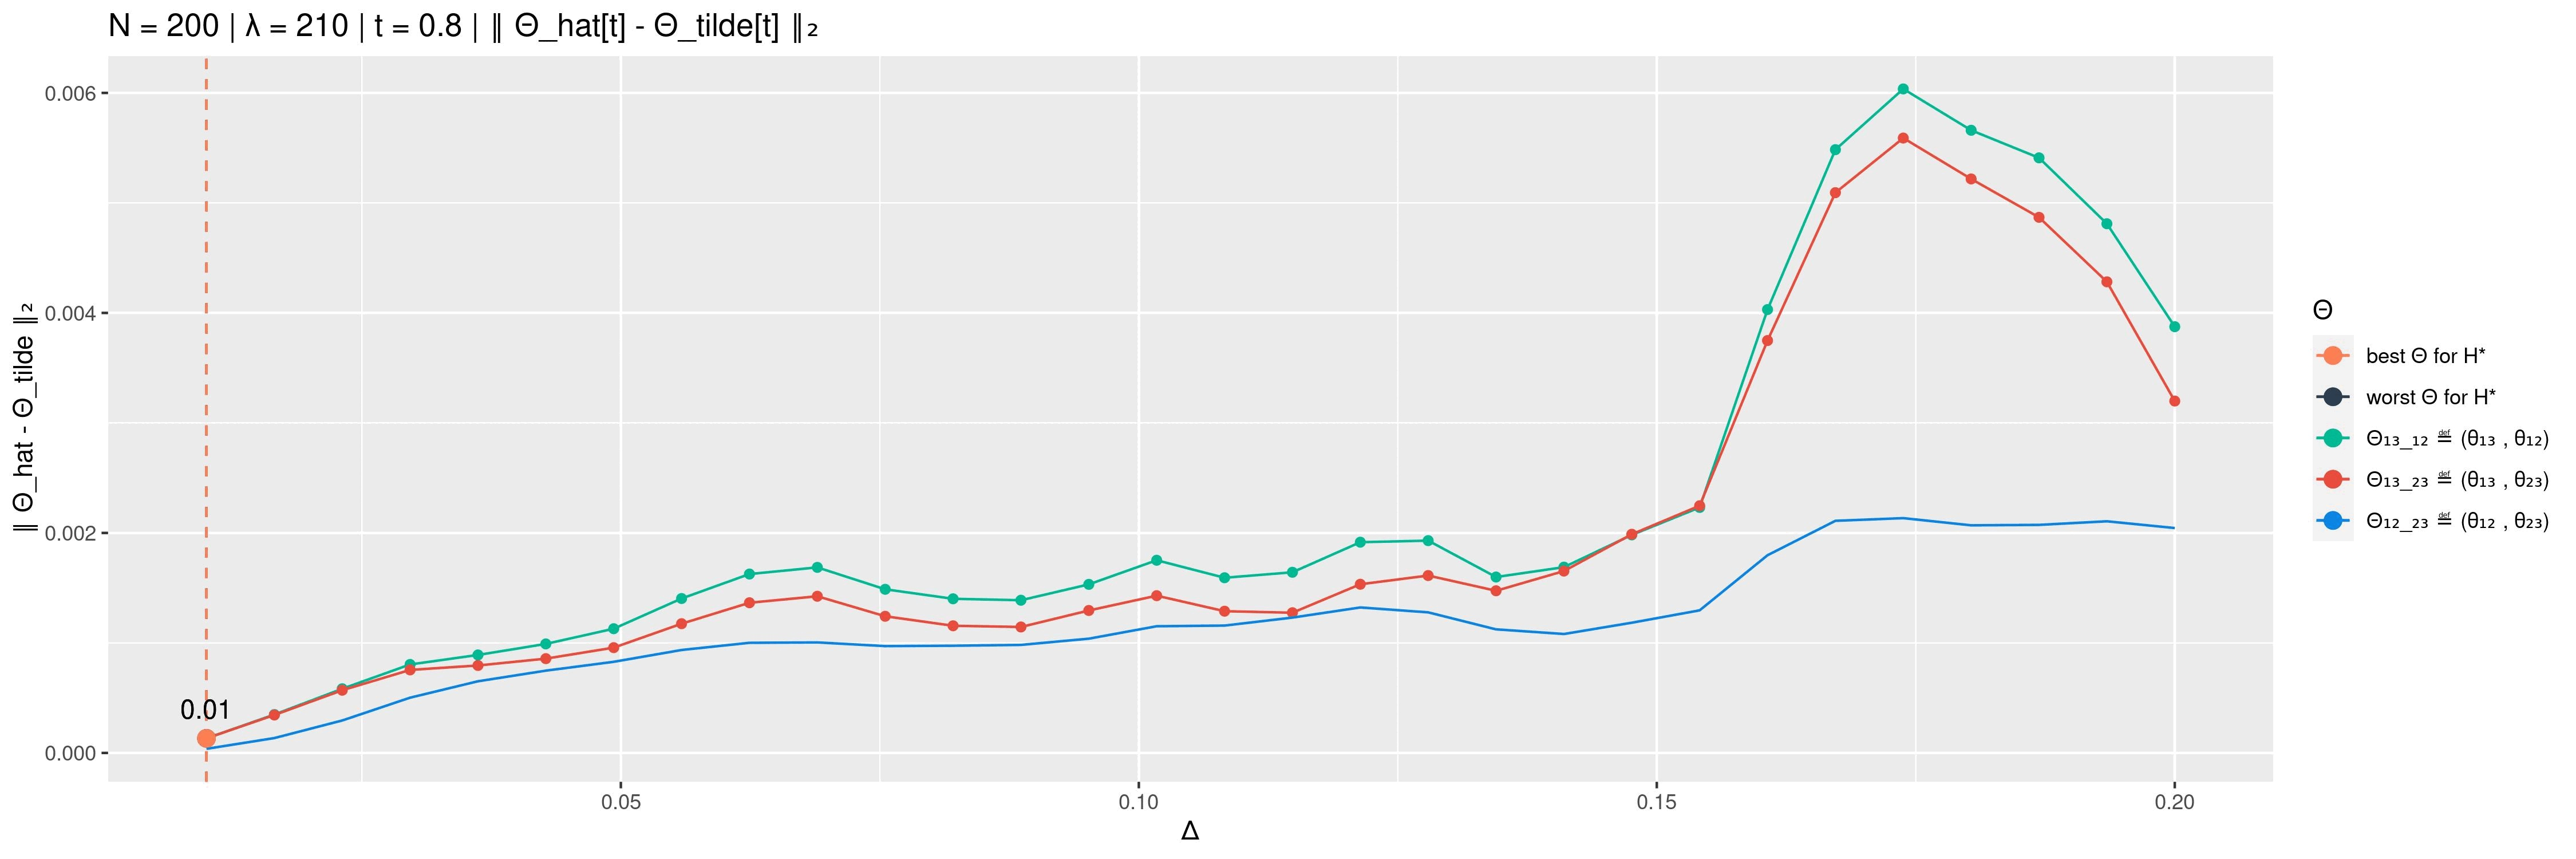
\includegraphics[width=0.8\textwidth]{Images/risque/N200_t0.8_lbd210.jpg}

	\label{fig:sparse_osef}
	\caption{Graphe des risques dans les cas \og sparse \fg et \og raisonnablement dense \fg}
\end{figure}

\pagebreak
\subsection{couple $\Theta$ : $1 \rightarrow 3$ / $1 \rightarrow 2$}

\begin{table}[H]
\centering
\begin{tabularx}{\textwidth}{ccccXXXX}
	\toprule
$t$ & $H_t$ & $N$      & $\lambda$ & différence $\operatorname{med} \mathcal R^{[\,abs\,]}_{mc}(\Theta, \Delta)$ & \textbf{meilleur} & différence  $\mathds V \mathcal R^{[\,abs\,]}_{mc}(\Theta, \Delta)$ & \textbf{meilleur} \\
	\midrule

	0.3 & 0.51  & $\vdots$ & $\vdots$  & 7.26                                                       & indiv             & 8.36                                               & indiv             \\
	0.4 & 0.55  & $\vdots$ & $\vdots$  & 6.31                                                       & indiv             & 6.91                                               & indiv             \\
	0.5 & 0.60  & $\vdots$ & $\vdots$  & 2.32                                                       & indiv             & 0.07                                               & indiv             \\
	0.6 & 0.65  & 200      & 45        & 0.09                                                       & indiv             & 13.68                                              & global            \\
	0.7 & 0.69  & $\vdots$ & $\vdots$  & 0.01                                                       & indiv             & 15.70                                              & global            \\
	0.8 & 0.73  & $\vdots$ & $\vdots$  & 0.22                                                       & indiv             & 0.02                                               & indiv             \\

	\midrule

	0.3 & 0.51  & $\vdots$ & $\vdots$  & 0.72                                                       & indiv             & 0.32                                               & indiv             \\
	0.4 & 0.55  & $\vdots$ & $\vdots$  & 0.79                                                       & indiv             & 0.36                                               & indiv             \\
	0.5 & 0.60  & $\vdots$ & $\vdots$  & 0.29                                                       & indiv             & 0.04                                               & indiv             \\
	0.6 & 0.65  & 200      & 90        & 0.01                                                       & indiv             & 9.93                                               & global            \\
	0.7 & 0.69  & $\vdots$ & $\vdots$  & 2$\cdot 10^{-3}$                                           & indiv             & 5$\cdot 10^{-6}$                                   & indiv             \\
	0.8 & 0.73  & $\vdots$ & $\vdots$  & 0.03                                                       & indiv             & 2$\cdot 10^{-3}$                                   & indiv             \\

	\midrule


	0.3 & 0.51  & $\vdots$ & $\vdots$  & 1$\cdot 10^{-3}$                                           & global            & 1$\cdot 10^{-5}$                                   & indiv             \\
	0.4 & 0.55  & $\vdots$ & $\vdots$  & 3$\cdot 10^{-3}$                                           & global            & 9$\cdot 10^{-5}$                                   & global            \\
	0.5 & 0.60  & $\vdots$ & $\vdots$  & 3$\cdot 10^{-5}$                                           & global            & 7$\cdot 10^{-6}$                                   & global            \\
	0.6 & 0.65  & 200      & 150       & 4$\cdot 10^{-6}$                                           & global            & 1$\cdot 10^{-7}$                                   & global            \\
	0.7 & 0.69  & $\vdots$ & $\vdots$  & 1$\cdot 10^{-6}$                                           & indiv             & 1$\cdot 10^{-8}$                                   & global            \\
	0.8 & 0.73  & $\vdots$ & $\vdots$  & 9$\cdot 10^{-6}$                                           & indiv             & 4$\cdot 10^{-6}$                                   & global            \\

	\midrule



	0.3 & 0.51  & $\vdots$ & $\vdots$  & 4$\cdot 10^{-3}$                                           & indiv             & 3$\cdot 10^{-5}$                                   & global            \\
	0.4 & 0.55  & $\vdots$ & $\vdots$  & 2$\cdot 10^{-3}$                                           & indiv             & 3$\cdot 10^{-6}$                                   & indiv             \\
	0.5 & 0.60  & $\vdots$ & $\vdots$  & 5$\cdot 10^{-5}$                                           & global            & 5$\cdot 10^{-7}$                                   & global            \\
	0.6 & 0.65  & 200      & 270       & 2$\cdot 10^{-4}$                                           & global            & 2$\cdot 10^{-7}$                                   & global            \\
	0.7 & 0.69  & $\vdots$ & $\vdots$  & 4$\cdot 10^{-4}$                                           & global            & 4$\cdot 10^{-6}$                                   & global            \\
	0.8 & 0.73  & $\vdots$ & $\vdots$  & 2$\cdot 10^{-4}$                                           & global            & 2$\cdot 10^{-7}$                                   & indiv             \\

	\midrule



	0.3 & 0.51  & $\vdots$ & $\vdots$  & 5$\cdot 10^{-3}$                                           & indiv             & 7$\cdot 10^{-5}$                                   & global            \\
	0.4 & 0.55  & $\vdots$ & $\vdots$  & 1$\cdot 10^{-3}$                                           & indiv             & 4$\cdot 10^{-6}$                                   & indiv             \\
	0.5 & 0.60  & $\vdots$ & $\vdots$  & 7$\cdot 10^{-5}$                                           & indiv             & 1$\cdot 10^{-7}$                                   & indiv             \\
	0.6 & 0.65  & 200      & 405       & 6$\cdot 10^{-5}$                                           & global            & 5$\cdot 10^{-9}$                                   & global            \\
	0.7 & 0.69  & $\vdots$ & $\vdots$  & 6$\cdot 10^{-5}$                                           & global            & 5$\cdot 10^{-9}$                                   & global            \\
	0.8 & 0.73  & $\vdots$ & $\vdots$  & 6$\cdot 10^{-5}$                                           & global            & 3$\cdot 10^{-9}$                                   & indiv             \\

	\bottomrule
\end{tabularx}
\caption{Comparaison de la médiane et de la variance du risque euclidien (absolu) entre lissage global et lissage individuel}
\label{tab:couple_1312_indiv_vs_glob}
\addcontentsline{lot}{table}{\numberline{} Comparaison de la distribution des risques entre la méthode de lissage \og individuelle \fg et \og globale \fg}
\end{table}

\subsection{couple $\Theta$ : $1 \rightarrow 3$ / $2 \rightarrow 3$}

% r$> diff(200, 45)                                                                                     
% [1] "- : indiv better | + : global better"                                                            
%     t       delta       mean      median        var          mad         q_05        q_25        q_75
% 1: 0.3  0.00000000 -7.6270828 -7.37026885 -8.2035235 -3.174973193 -3.754290748 -5.35134678 -9.57294123
% 2: 0.4  0.00000000 -6.6368521 -6.11751969 -7.4471987 -2.627601546 -3.029439978 -4.79160190 -8.51104316
% 3: 0.5 -0.07862069 -0.2934719 -0.38050702  0.8432740 -0.227736636 -0.103390660 -0.24313694 -0.56350343
% 4: 0.6 -0.01965517  0.2600751 -0.02028208 14.3548827 -0.007235096 -0.009493182 -0.01566113 -0.02648008
% 5: 0.7  0.00000000  0.2617239 -0.01360111 15.3379846 -0.006420801 -0.006145075 -0.01020567 -0.01950629
% 6: 0.8  0.00000000 -1.0286618 -0.98957933 -0.1277138 -0.328730739 -0.513711899 -0.77282139 -1.22231386

% r$> diff(200, 90)
% [1] "- : indiv better | + : global better"
%      t        delta         mean       median           var          mad          q_05         q_25
% 1: 0.3  0.176896552 -0.856585871 -0.719384529 -3.408459e-01 -0.514250932 -0.1482161512 -0.428558025
% 2: 0.4  0.000000000 -0.848029325 -0.746247416 -2.900853e-01 -0.506689330 -0.1693310177 -0.454365167
% 3: 0.5 -0.190000000 -0.088082194 -0.063735717 -5.923914e-03 -0.045997470 -0.0119902282 -0.040013634
% 4: 0.6 -0.045862069  0.224528663 -0.005515365  1.053572e+01 -0.003678725 -0.0014378368 -0.003555736
% 5: 0.7  0.006551724 -0.002702045 -0.002349014 -5.853071e-06 -0.001523825 -0.0006885826 -0.001469197
% 6: 0.8  0.006551724 -0.163403173 -0.148092871 -8.046940e-03 -0.085036474 -0.0473962445 -0.097395710

% r$> diff(200, 150)
% [1] "- : indiv better | + : global better"
%     t      delta          mean        median           var           mad          q_05          q_25
% 1: 0.3 0.00000000  1.246107e-03  1.601503e-03 -2.931575e-05 -1.248625e-03  1.635929e-03  2.083005e-03
% 2: 0.4 0.01310345  1.715370e-03  3.816957e-05  2.265213e-04  2.713487e-04  7.661585e-05  2.407706e-04
% 3: 0.5 0.00000000 -8.161825e-04 -2.647296e-05 -6.059787e-06 -3.979208e-05 -2.503312e-06 -6.398483e-06
% 4: 0.6 0.00000000 -6.404176e-05  3.825901e-06 -1.172869e-07 -1.165347e-05  4.649156e-06  1.186941e-05
% 5: 0.7 0.00000000 -3.687266e-06  9.947828e-06 -2.473056e-08 -1.426801e-05  7.418619e-06  2.516984e-05
% 6: 0.8 0.00000000 -7.141958e-04 -7.041524e-06 -3.265788e-06 -2.476943e-05  3.642897e-06  5.614608e-06

% r$> diff(200, 270)                                                                                    
% [1] "- : indiv better | + : global better"                                                            
%     t       delta          mean        median           var           mad          q_05          q_25
% 1: 0.3 0.013103448 -0.0033432119 -2.773041e-03 -1.880183e-05 -3.538987e-04 -2.205794e-03 -2.398762e-03
% 2: 0.4 0.000000000 -0.0006474065 -9.601704e-04  5.472988e-06 -3.545330e-04 -4.641782e-04 -4.132294e-04
% 3: 0.5 0.013103448  0.0001666614  7.558968e-05  4.607552e-07  9.103183e-05  3.292461e-06  2.366847e-05
% 4: 0.6 0.006551724  0.0002899463  2.672173e-04  1.665197e-07  1.781080e-04  6.189276e-05  1.496751e-04
% 5: 0.7 0.013103448  0.0005959056  4.196224e-04  4.435436e-06  3.324503e-04  6.585841e-05  1.980760e-04
% 6: 0.8 0.006551724  0.0001634511  2.087072e-04 -7.233077e-08  1.169489e-04  5.273427e-05  1.233876e-04

% r$> diff(200, 405)                                                                       
% [1] "- : indiv better | + : global better"
%     t        delta          mean        median           var           mad          q_05
% 1: 0.3  0.000000000 -3.376705e-03 -3.198646e-03 -1.940232e-05 -4.232165e-04 -1.210571e-03
% 2: 0.4 -0.045862069 -7.354738e-04 -4.400388e-04 -4.386017e-06 -2.896975e-04  9.388869e-05
% 3: 0.5 -0.006551724 -6.027816e-05 -1.519413e-06 -3.477833e-07 -1.503831e-07 -5.982584e-08
% 4: 0.6  0.000000000  6.653227e-05  6.389595e-05  5.594693e-09  2.986906e-05  1.961957e-05
% 5: 0.7  0.000000000  6.582442e-05  5.363359e-05  6.117996e-09  3.528404e-05  1.652330e-05
% 6: 0.8  0.000000000  4.691333e-05  5.266891e-05 -2.009986e-08  2.971988e-05  2.742132e-05
\begin{table}[H]
\begin{tabularx}{\textwidth}{ccccXXXX}
	\toprule
$t$ & $H_t$ & $N$      & $\lambda$ & différence $\operatorname{med} \mathcal R^{[\,abs\,]}_{mc}(\Theta, \Delta)$ & \textbf{meilleur} & différence  $\mathds V \mathcal R^{[\,abs\,]}_{mc}(\Theta, \Delta)$ & \textbf{meilleur} \\
	\midrule

	0.3 & 0.51  & $\vdots$ & $\vdots$  & 7.37                                                       & indiv             & 8.20                                               & indiv             \\
	0.4 & 0.55  & $\vdots$ & $\vdots$  & 6.12                                                       & indiv             & 7.44                                               & indiv             \\
	0.5 & 0.60  & $\vdots$ & $\vdots$  & 3.80                                                       & indiv             & 0.84                                               & global            \\
	0.6 & 0.65  & 200      & 45        & 0.02                                                       & indiv             & 14.35                                              & global            \\
	0.7 & 0.69  & $\vdots$ & $\vdots$  & 1$\cdot 10^{-2}$                                           & indiv             & 15.33                                              & global            \\
	0.8 & 0.73  & $\vdots$ & $\vdots$  & 9.90                                                       & indiv             & 0.13                                               & indiv             \\

	\midrule

	0.3 & 0.51  & $\vdots$ & $\vdots$  & 7.19                                                       & indiv             & 3.40                                               & indiv             \\
	0.4 & 0.55  & $\vdots$ & $\vdots$  & 7.46                                                       & indiv             & 2.90                                               & indiv             \\
	0.5 & 0.60  & $\vdots$ & $\vdots$  & 6.37                                                       & indiv             & 0.59                                               & indiv             \\
	0.6 & 0.65  & 200      & 90        & 5$\cdot 10^{-3}$                                           & indiv             & 10.53                                              & global            \\
	0.7 & 0.69  & $\vdots$ & $\vdots$  & 2$\cdot 10^{-3}$                                           & indiv             & 5$\cdot 10^{-6}$                                   & indiv             \\
	0.8 & 0.73  & $\vdots$ & $\vdots$  & 1$\cdot 10^{-1}$                                           & indiv             & 8$\cdot 10^{-3}$                                   & indiv             \\

	\midrule

	0.3 & 0.51  & $\vdots$ & $\vdots$  & 1$\cdot 10^{-3}$                                           & global            & 2$\cdot 10^{-5}$                                   & indiv             \\
	0.4 & 0.55  & $\vdots$ & $\vdots$  & 3$\cdot 10^{-5}$                                           & global            & 2$\cdot 10^{-4}$                                   & global            \\
	0.5 & 0.60  & $\vdots$ & $\vdots$  & 2$\cdot 10^{-5}$                                           & indiv             & 6$\cdot 10^{-6}$                                   & indiv             \\
	0.6 & 0.65  & 200      & 150       & 4$\cdot 10^{-6}$                                           & global            & 1$\cdot 10^{-7}$                                   & indiv             \\
	0.7 & 0.69  & $\vdots$ & $\vdots$  & 1$\cdot 10^{-5}$                                           & global            & 2$\cdot 10^{-8}$                                   & indiv             \\
	0.8 & 0.73  & $\vdots$ & $\vdots$  & 7$\cdot 10^{-6}$                                           & indiv             & 3$\cdot 10^{-6}$                                   & indiv             \\

	\midrule

	0.3 & 0.51  & $\vdots$ & $\vdots$  & 2$\cdot 10^{-3}$                                           & indiv             & 1$\cdot 10^{-5}$                                   & indiv             \\
	0.4 & 0.55  & $\vdots$ & $\vdots$  & 1$\cdot 10^{-3}$                                           & indiv             & 5$\cdot 10^{-6}$                                   & global            \\
	0.5 & 0.60  & $\vdots$ & $\vdots$  & 7$\cdot 10^{-5}$                                           & global            & 4$\cdot 10^{-7}$                                   & global            \\
	0.6 & 0.65  & 200      & 270       & 3$\cdot 10^{-4}$                                           & global            & 1$\cdot 10^{-7}$                                   & global            \\
	0.7 & 0.69  & $\vdots$ & $\vdots$  & 4$\cdot 10^{-4}$                                           & global            & 4$\cdot 10^{-6}$                                   & global            \\
	0.8 & 0.73  & $\vdots$ & $\vdots$  & 2$\cdot 10^{-4}$                                           & global            & 7$\cdot 10^{-8}$                                   & indiv             \\

	\midrule


	0.3 & 0.51  & $\vdots$ & $\vdots$  & 3$\cdot 10^{-3}$                                           & indiv             & 1$\cdot 10^{-5}$                                   & indiv             \\
	0.4 & 0.55  & $\vdots$ & $\vdots$  & 4$\cdot 10^{-4}$                                           & indiv             & 4$\cdot 10^{-6}$                                   & indiv             \\
	0.5 & 0.60  & $\vdots$ & $\vdots$  & 2$\cdot 10^{-5}$                                           & indiv             & 3$\cdot 10^{-7}$                                   & indiv             \\
	0.6 & 0.65  & 200      & 405       & 6$\cdot 10^{-5}$                                           & global            & 5$\cdot 10^{-9}$                                   & global            \\
	0.7 & 0.69  & $\vdots$ & $\vdots$  & 5$\cdot 10^{-5}$                                           & global            & 6$\cdot 10^{-9}$                                   & global            \\
	0.8 & 0.73  & $\vdots$ & $\vdots$  & 5$\cdot 10^{-5}$                                           & global            & 2$\cdot 10^{-8}$                                   & indiv             \\

	\bottomrule
\end{tabularx}
\caption{Comparaison de la médiane et de la variance du risque euclidien (absolu) entre lissage global et lissage individuel}
\label{tab:couple_1323_indiv_vs_glob}
\end{table}

% ------- Δ = 0.125 -------
% min :1.14718987543925e-05
% max :22.2868913474062
% q_97.5 : c(`97.5%` = 0.0152186598332864)
% q_95 :c(`95%` = 0.00915432362046129)
% [1] "➤ quantiles extrêmes (> 97.5%) :"
% mc eucl_12_13
% 1:   6  0.1968115
% 2:  91  0.1810575
% 3: 109 13.5030314
% 4: 133  0.1432259
% 5: 157 22.2868913
% ------- Δ = 0.062 -------
%   min :4.35276546353077e-06
% max :67.8923793508904
% q_97.5 : c(`97.5%` = 0.00488494583251508)
% q_95 :c(`95%` = 0.00357287390908308)
% [1] "➤ quantiles extrêmes (> 97.5%) :"
% mc   eucl_12_13
% 1:  6 67.892379351
% 2: 18  0.007600918
% 3: 33  0.005005537
% 4: 67  0.006323381
% 5: 90  0.005215573

\begin{table}[H]
\centering
	\begin{tabularx}{\textwidth}{ccccc}
		\toprule
statistique sur $\widehat{\mathcal R}_{mc}^{[\,abs\,]}$ & \textbf{Individuel} & \textbf{Global}    & $\Delta$ & $\lambda$ \\
		\midrule
		\textbf{min}                        & 0.000226            & 0.338              & 0.1      & $\vdots$  \\
		\textbf{max}                        & 36.71               & 2.448              & 0.1      & 60        \\
		\textbf{quantile} $q_{97.5\%}$      & 0.0618              & 1.862              & 0.1      & $\vdots$  \\
		\textbf{quantile} $q_{95\%}$        & 0.0457              & 1.682              & 0.1      & $\vdots$  \\
		\midrule
		\textbf{min}                        & 3.06$\cdot 10^{-6}$ & 0.474              & 0.015    & $\vdots$  \\
		\textbf{max}                        & 83.53               & 2.825              & 0.015    & $\vdots$  \\
		\textbf{quantile} $q_{97.5\%}$      & 0.00322             & 1.909              & 0.015    & 60        \\
		\textbf{quantile} $q_{95\%}$        & 0.00236             & 1.794              & 0.015    & $\vdots$  \\

		\bottomrule

		\toprule
		% indiv :
		% ------- 210 = λ | Δ = 0.062 -------
		% min :4.35276546353077e-06
		% max :67.8923793508904
		% q_97.5 : c(`97.5%` = 0.00488494583251508)
		% q_95 :c(`95%` = 0.00357287390908308)
		% [1] "➤ quantiles extrêmes (> 97.5%) :"
		% mc   eucl_12_13
		% 1:  6 67.892379351
		% 2: 18  0.007600918
		% 3: 33  0.005005537
		% 4: 67  0.006323381
		% 5: 90  0.005215573
		% global :
		% ------- 210 = λ | Δ = 0.062 -------
		% min :6.61144132120086e-06
		% max :0.0104890373376202
		% q_97.5 : c(`97.5%` = 0.00459557879651001)
		% q_95 :c(`95%` = 0.00351969921068665)
		% mc  eucl_12_13
		% 1:  16 0.005841957
		% 2:  43 0.004847784
		% 3:  77 0.005425894
		% 4: 171 0.005126495
		% 5: 179 0.010489037
		\textbf{min}                        & 4$\cdot 10^{-6}$    & 6$\cdot 10^{-6}$   & 0.062    & $\vdots$  \\
		\textbf{max}                        & 67.89               & 0.01               & 0.062    & 210       \\
		\textbf{quantile} $q_{97.5\%}$      & 4.9$\cdot 10^{-3}$  & 4.6$\cdot 10^{-3}$ & 0.062    & $\vdots$  \\
		\textbf{quantile} $q_{95\%}$        & 3.6$\cdot 10^{-3}$  & 3.5$\cdot 10^{-3}$ & 0.062    & $\vdots$  \\

		\bottomrule
	\end{tabularx}
	\caption{Quelques statistiques sur la distribution du risque euclidien en fonction de la méthode de sélection de la fenêtre de lissage}
	\label{tab:stat_R_eucl_min_max_q}
\addcontentsline{lot}{table}{\numberline{} Données aberrantes dans les échantillons de Monte-Carlo pour le risque euclidien (non relatif)}
\end{table}



% ~ INDIV
% -------Δ = 0.1 - ------
% min:0.000225584627884278
% max:36.7108493938516
% q_97.5:c(`97.5%` = 0.0617630505148869)
% q_95:c(`95%` = 0.0456530021210119)
% -------Δ = 0.015 - ------
%     min:3.06408542204381e-06
% max:83.5292251521978
% q_97.5:c(`97.5%` = 0.00321982597686206)
% q_95:c(`95%` = 0.00236197723089737)
% ~ GLOBAL
% -------Δ = 0.1 - ------
% min:0.338299103983652
% max:2.44757683316762
% q_97.5:c(`97.5%` = 1.86152076412267)
% q_95:c(`95%` = 1.68205548116428)
% -------Δ = 0.015 - ------
% min:0.474057352714499
% max:2.82498526036493
% q_97.5:c(`97.5%` = 1.90935787150105)
% q_95:c(`95%` = 1.79403703076924)

\warn{
	Dans l'ensemble des graphes suivants se trouve une erreur de labélisation des graphes : La métrique $\mathcal R$ considérée est bel et bien la norme euclidienne \textbf{au carré} $\mathcal R ( \Theta , \Delta) = {\distnorme 2 {\widehat \Theta} {\widetilde \Theta}}^2$.
}

\begin{figure}[H]
	\centering
	\begin{minipage}{\linewidth}
		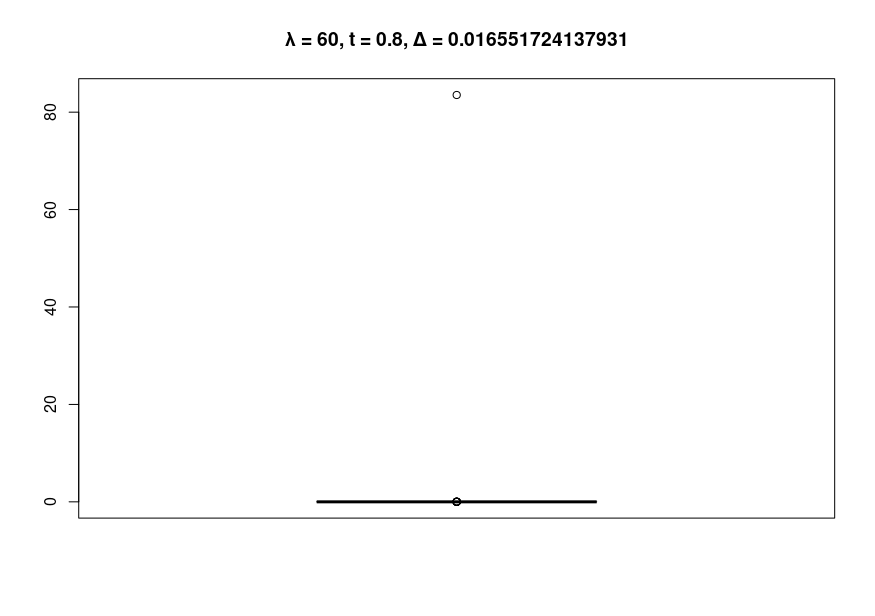
\includegraphics[width=0.47\textwidth]{Images/indiv_vs_glob/qq160.png}
		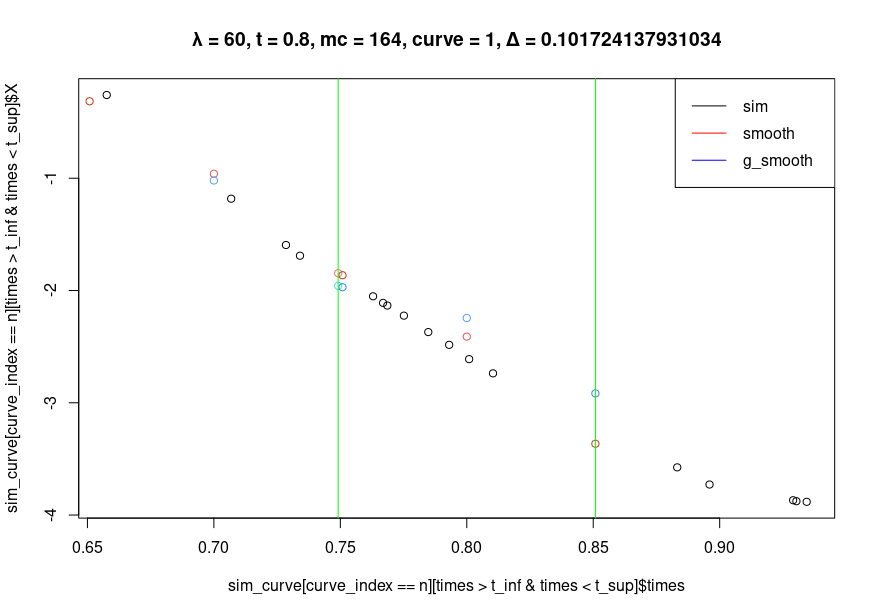
\includegraphics[width=0.47\textwidth]{Images/indiv_vs_glob/lbd60mc164c1.png}
	\end{minipage}

	\begin{minipage}{\linewidth}
		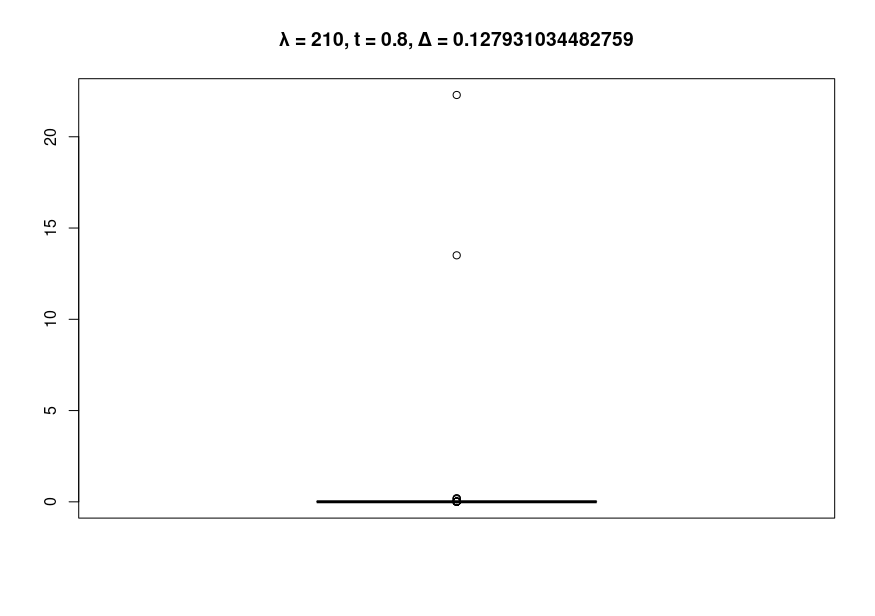
\includegraphics[width=0.47\textwidth]{Images/indiv_vs_glob/qq210.png}
		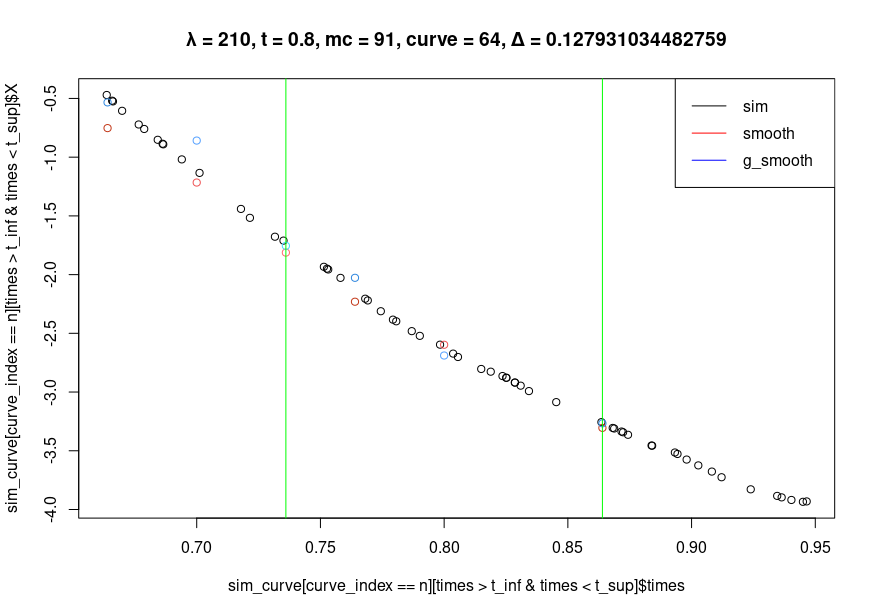
\includegraphics[width=0.47\textwidth]{Images/indiv_vs_glob/lbd210_mc91_c64.png}
	\end{minipage}
	\caption{Distribution des risques et aperçu d'une courbe pour un échantillon de monte carlo extrême sur le risque euclidien.}
	\label{fig:dist_R_eucl_curves}
\end{figure}

\begin{figure}[H]
	\centering
	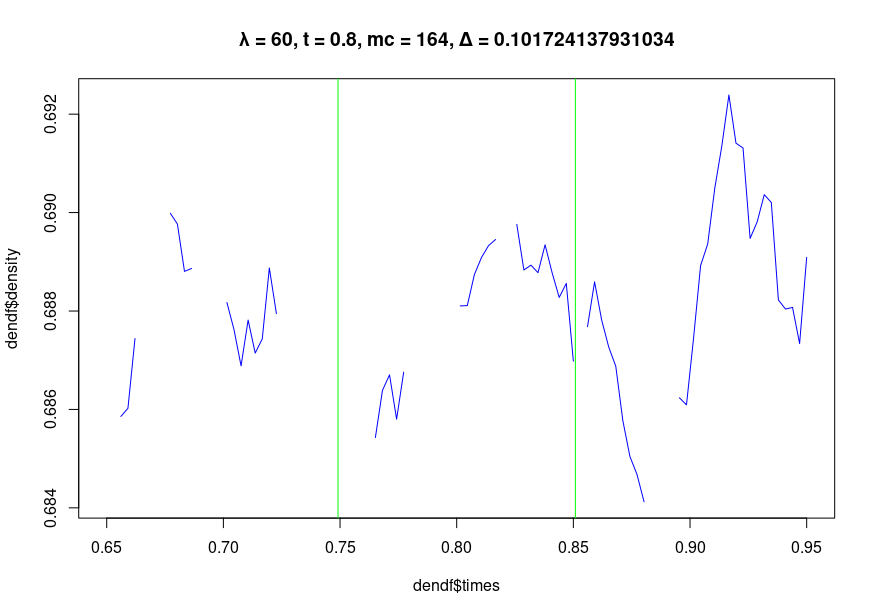
\includegraphics[width=0.7\textwidth]{Images/indiv_vs_glob/Tdensity_lbd60_mc164.png}
	\caption{Densité de points observés sur $[0.65, 0.95]$ pour $\lambda = 60$ sur un échantillon de monte carlo extrême, en un $\Delta$ problématique.}
	\label{fig:den_ex}
\end{figure}


\begin{figure}[H]
	\centering
	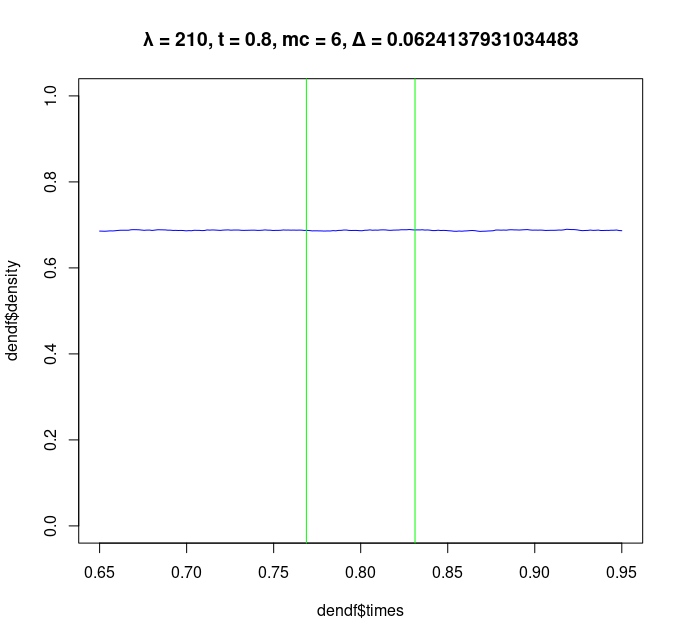
\includegraphics[width=0.7\textwidth]{Images/indiv_vs_glob/worst_210_67_mc6.png}
	\caption{Densité des points observés correspondant à la courbe présentée sur la figure \ref{fig:dist_R_eucl_curves}.}
	\label{fig:den_counterex}
\end{figure}



% N = 200	|
% λ = 90	|



% N = 200	|	
% λ = 210	|	


\begin{figure}[H]
	\centering

	\textbf{avec extrêmes : global}

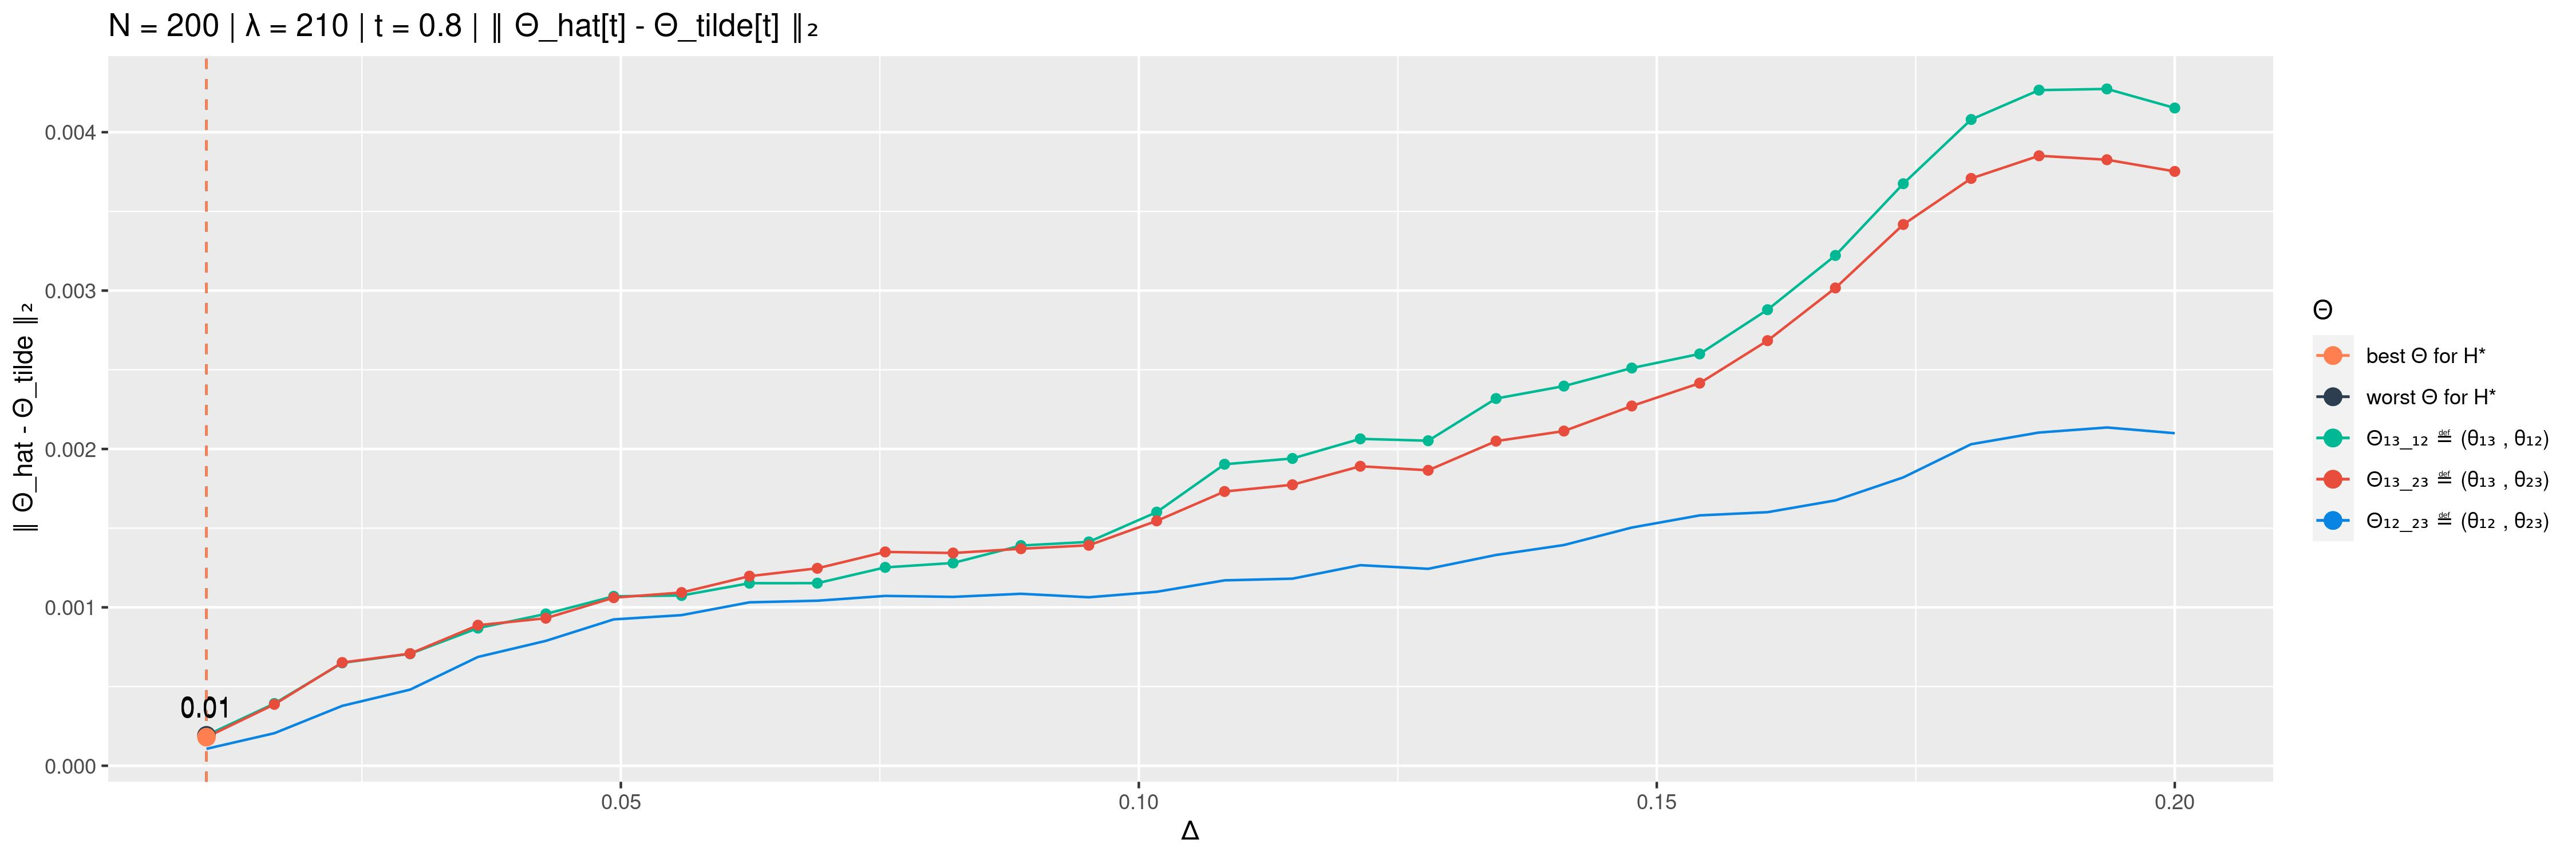
\includegraphics[width=0.9\textwidth]{Images/indiv_glob_img/compare/210_regular/all_glob.jpg}

	\textbf{avec extrêmes : individuel}

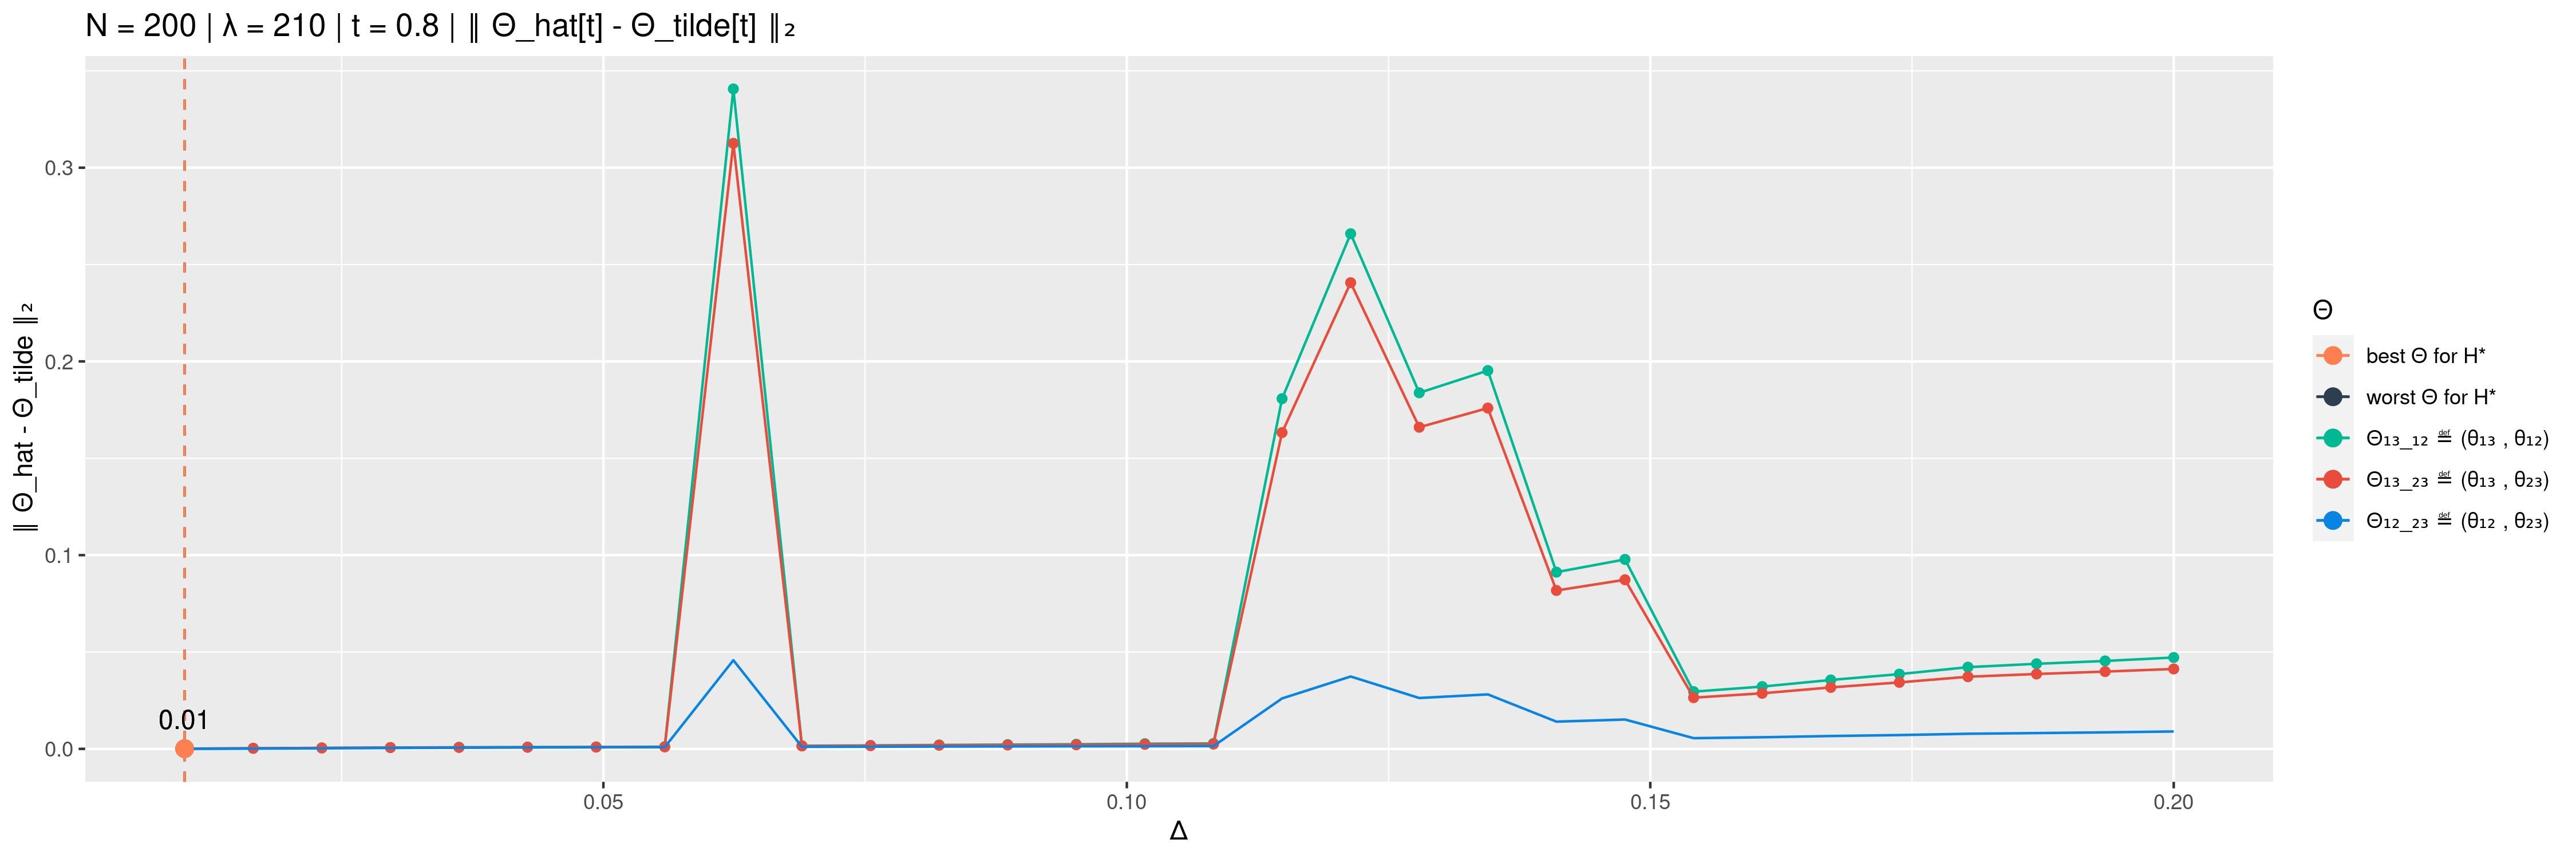
\includegraphics[width=0.9\textwidth]{Images/indiv_glob_img/compare/210_regular/all.jpg}

\textbf{sans extrêmes : global} (- top 2\%)
% TODO : changer d image : mauvais N, prendre N=200
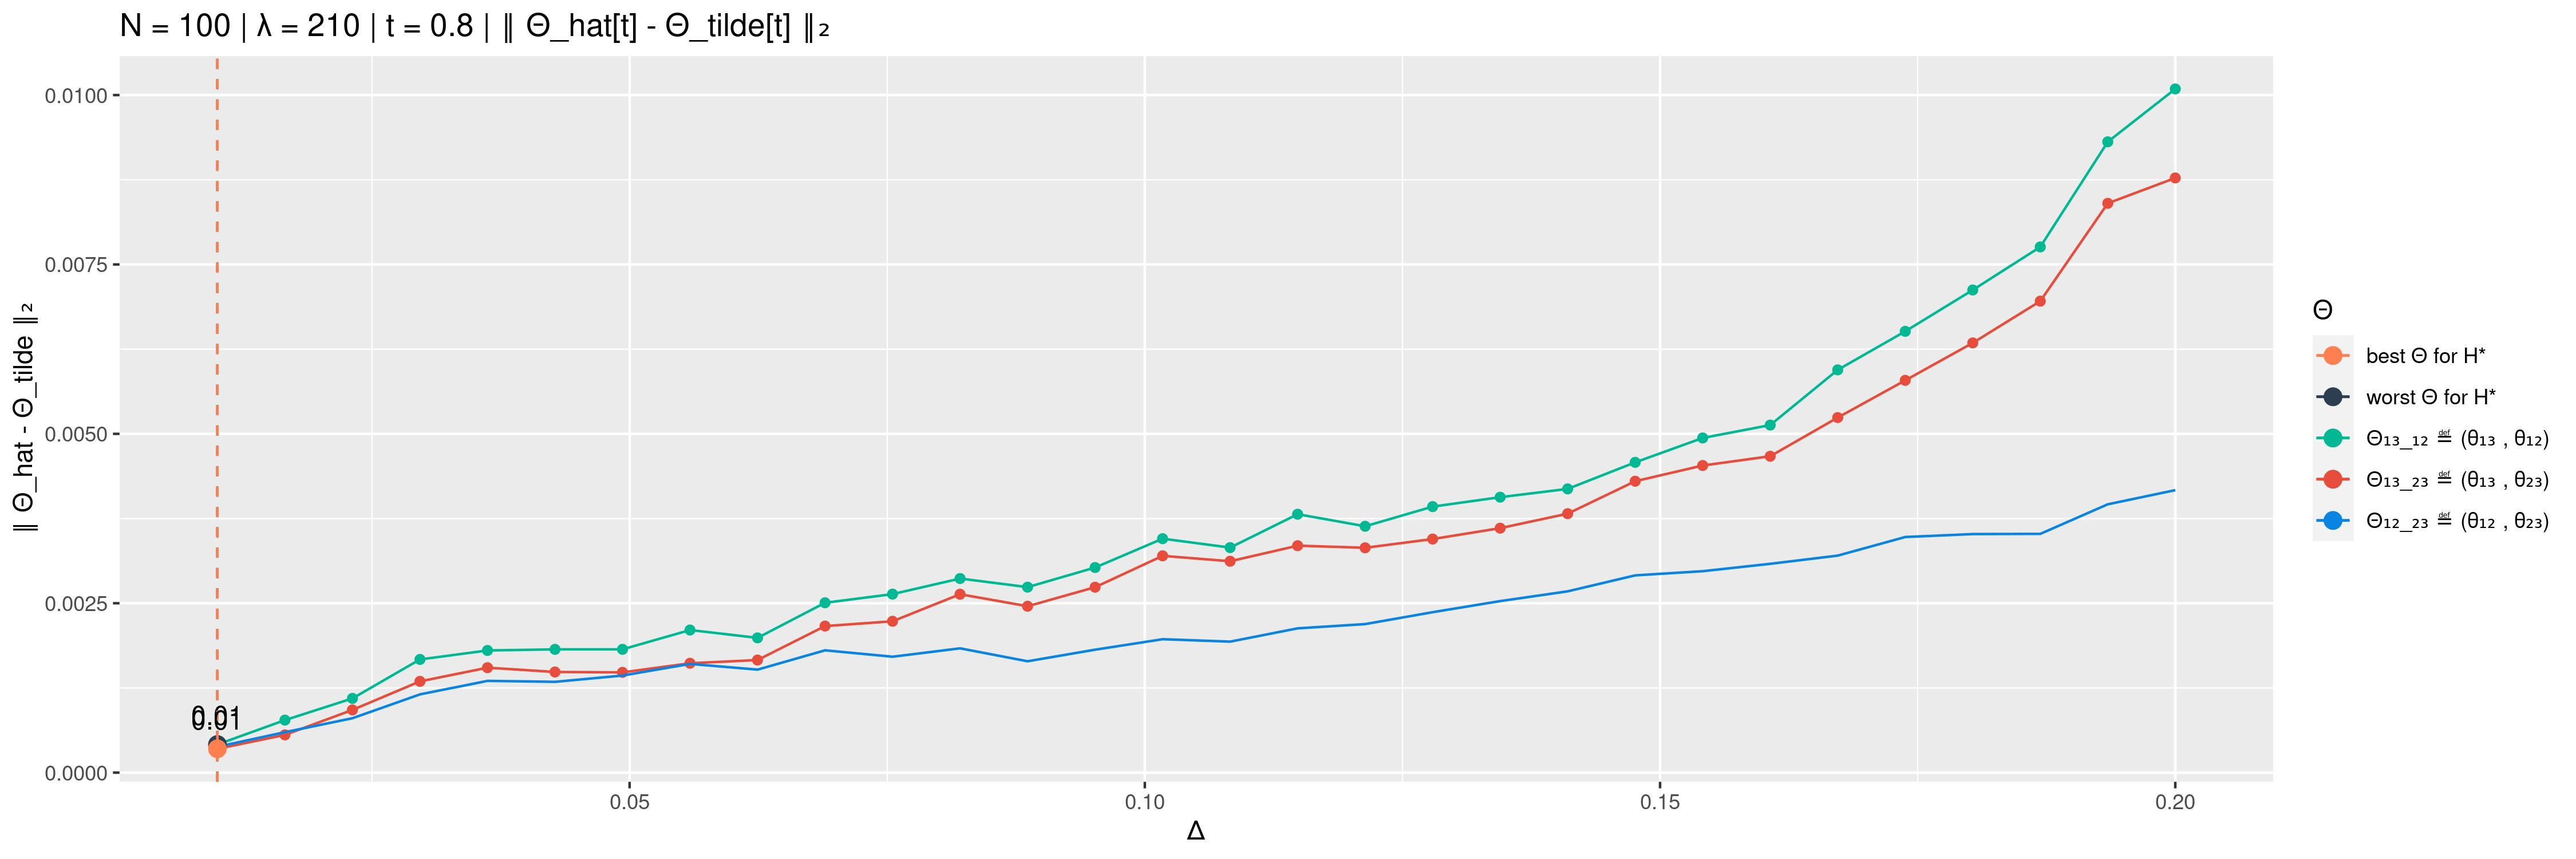
\includegraphics[width=0.9\textwidth]{Images/indiv_glob_img/compare/210_regular/no_xtrm_glob.jpg}

	\textbf{sans extrêmes : individuel} (- top 2\%)

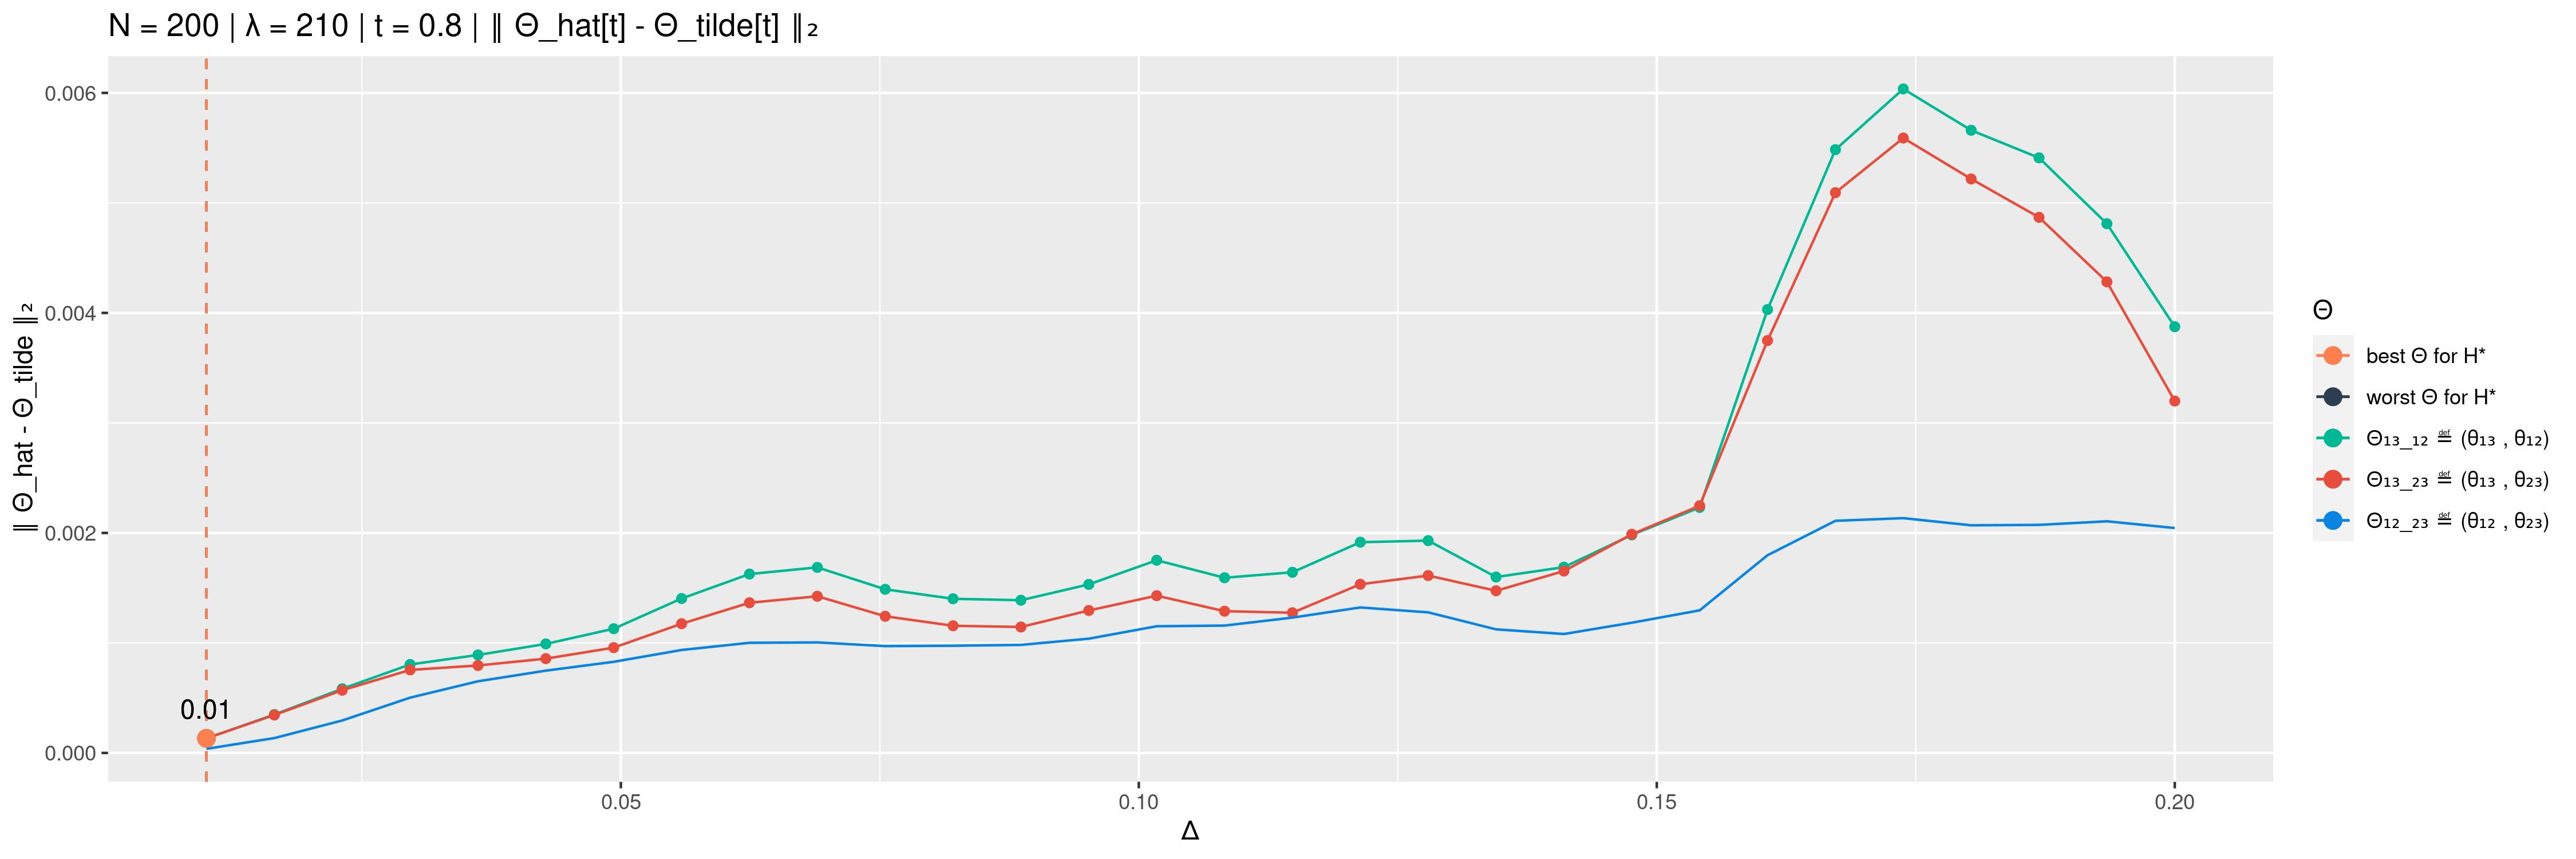
\includegraphics[width=0.9\textwidth]{Images/indiv_glob_img/compare/210_regular/no_xtrm.jpg}


	\caption{Risque Euclidien pour $N=200$, $\lambda=210$ en un point régulier selon la méthode utilisée pour la fenêtre de lissage}
	\label{fig:compare_xtrm_2}
\end{figure}

\begin{figure}[H]
	\centering
	\textbf{ H = 0.51 }

	Sparse :

	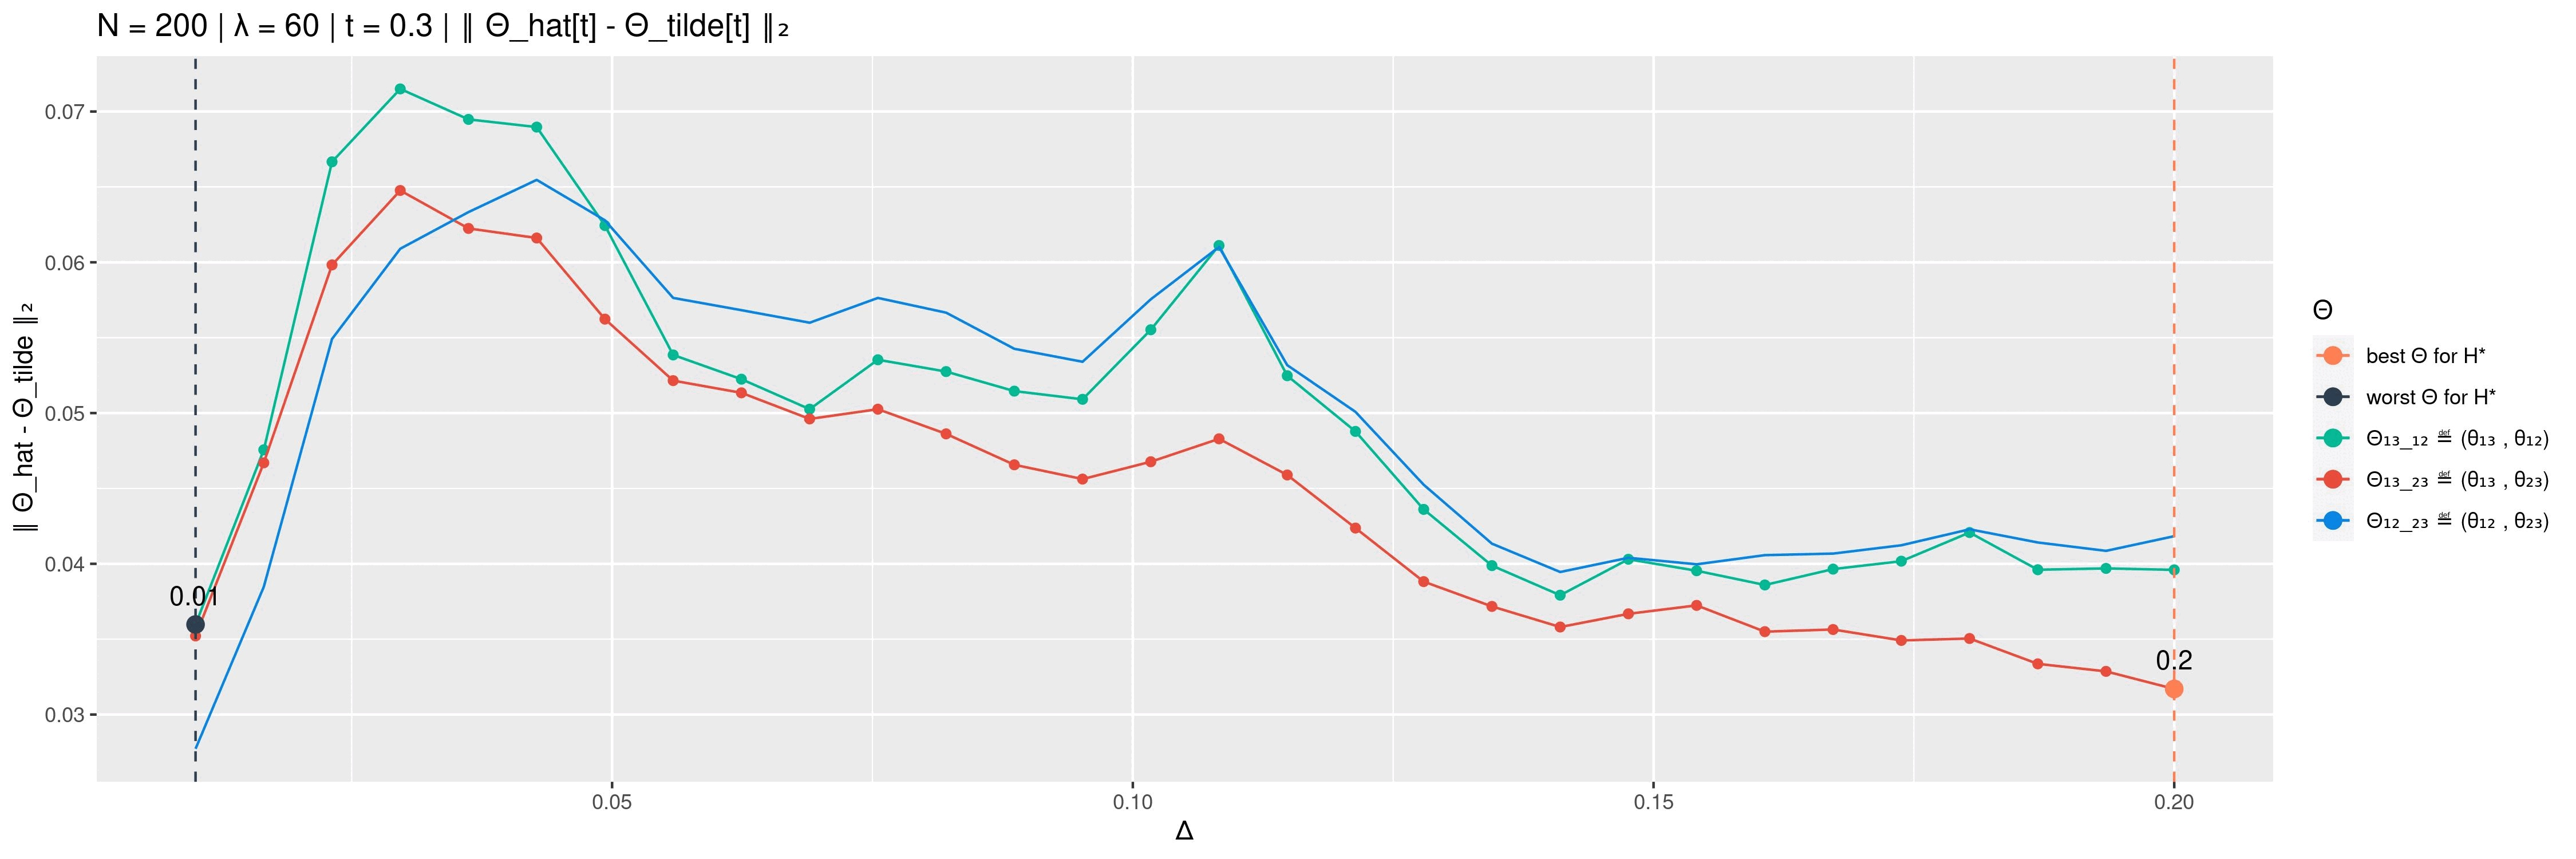
\includegraphics[width=0.8\textwidth]{Images/risque/N200_t0.3_lbd60.jpg}

	Dense :

	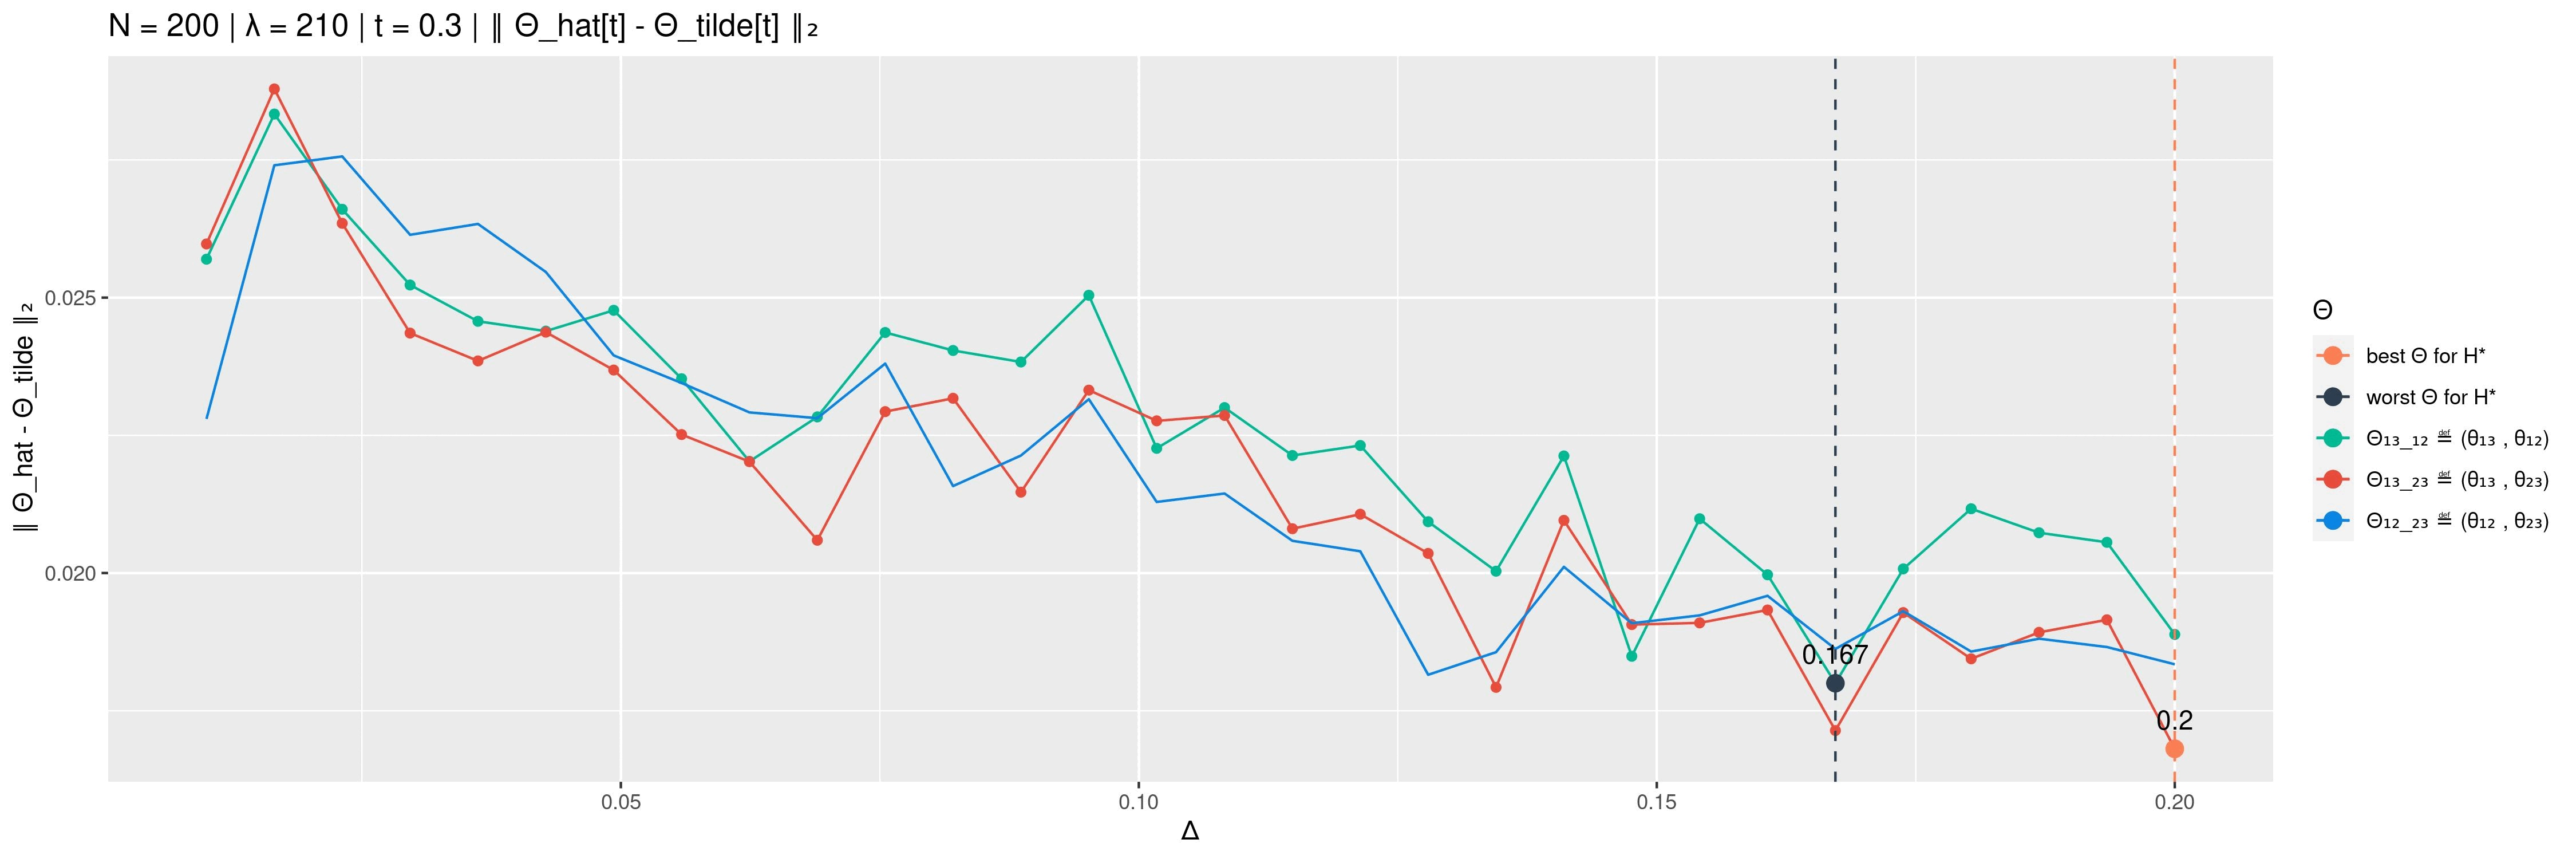
\includegraphics[width=0.8\textwidth]{Images/risque/N200_t0.3_lbd210.jpg}
\end{figure}

\begin{figure}[H]
	\centering
	\textbf{ H = 0.6 }

	Sparse :

	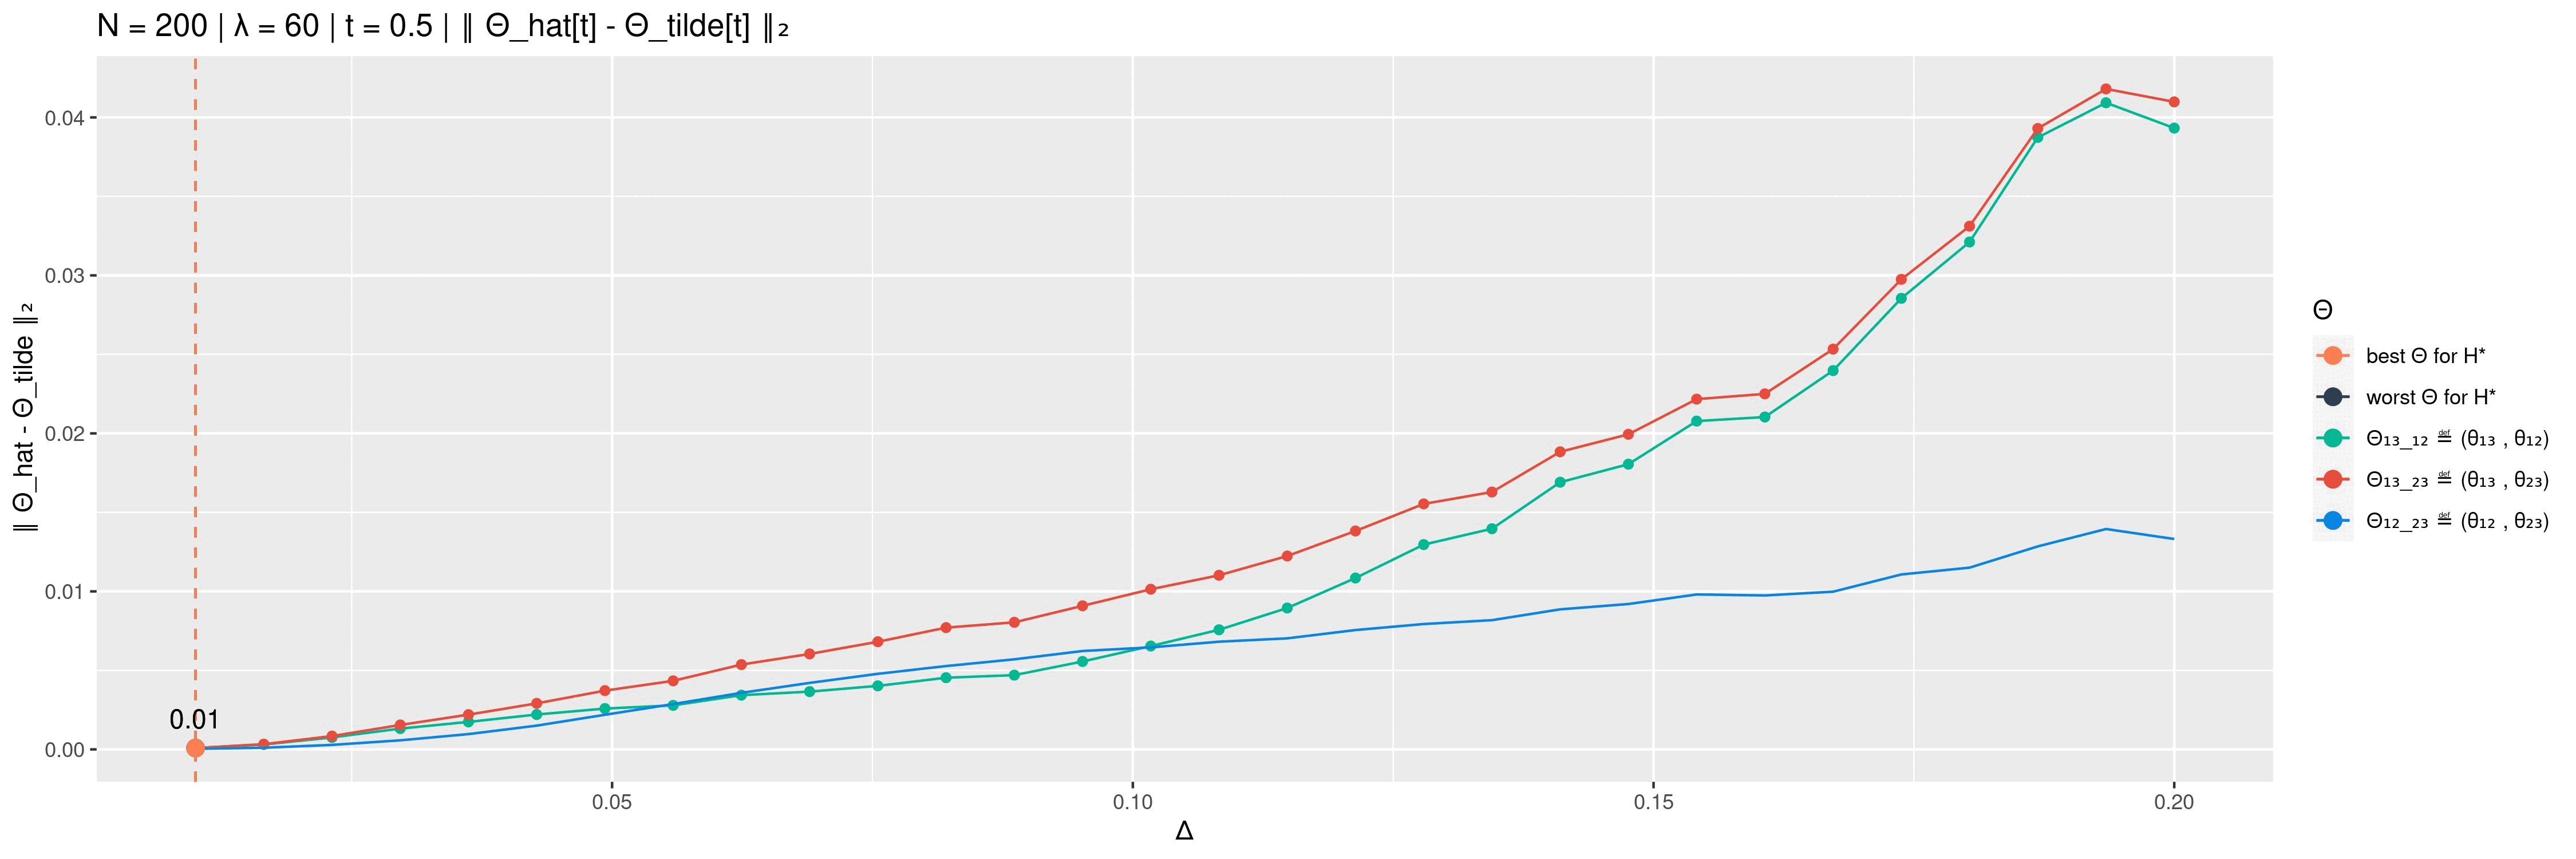
\includegraphics[width=0.8\textwidth]{Images/risque/N200_t0.5_lbd60.jpg}

	Dense :

	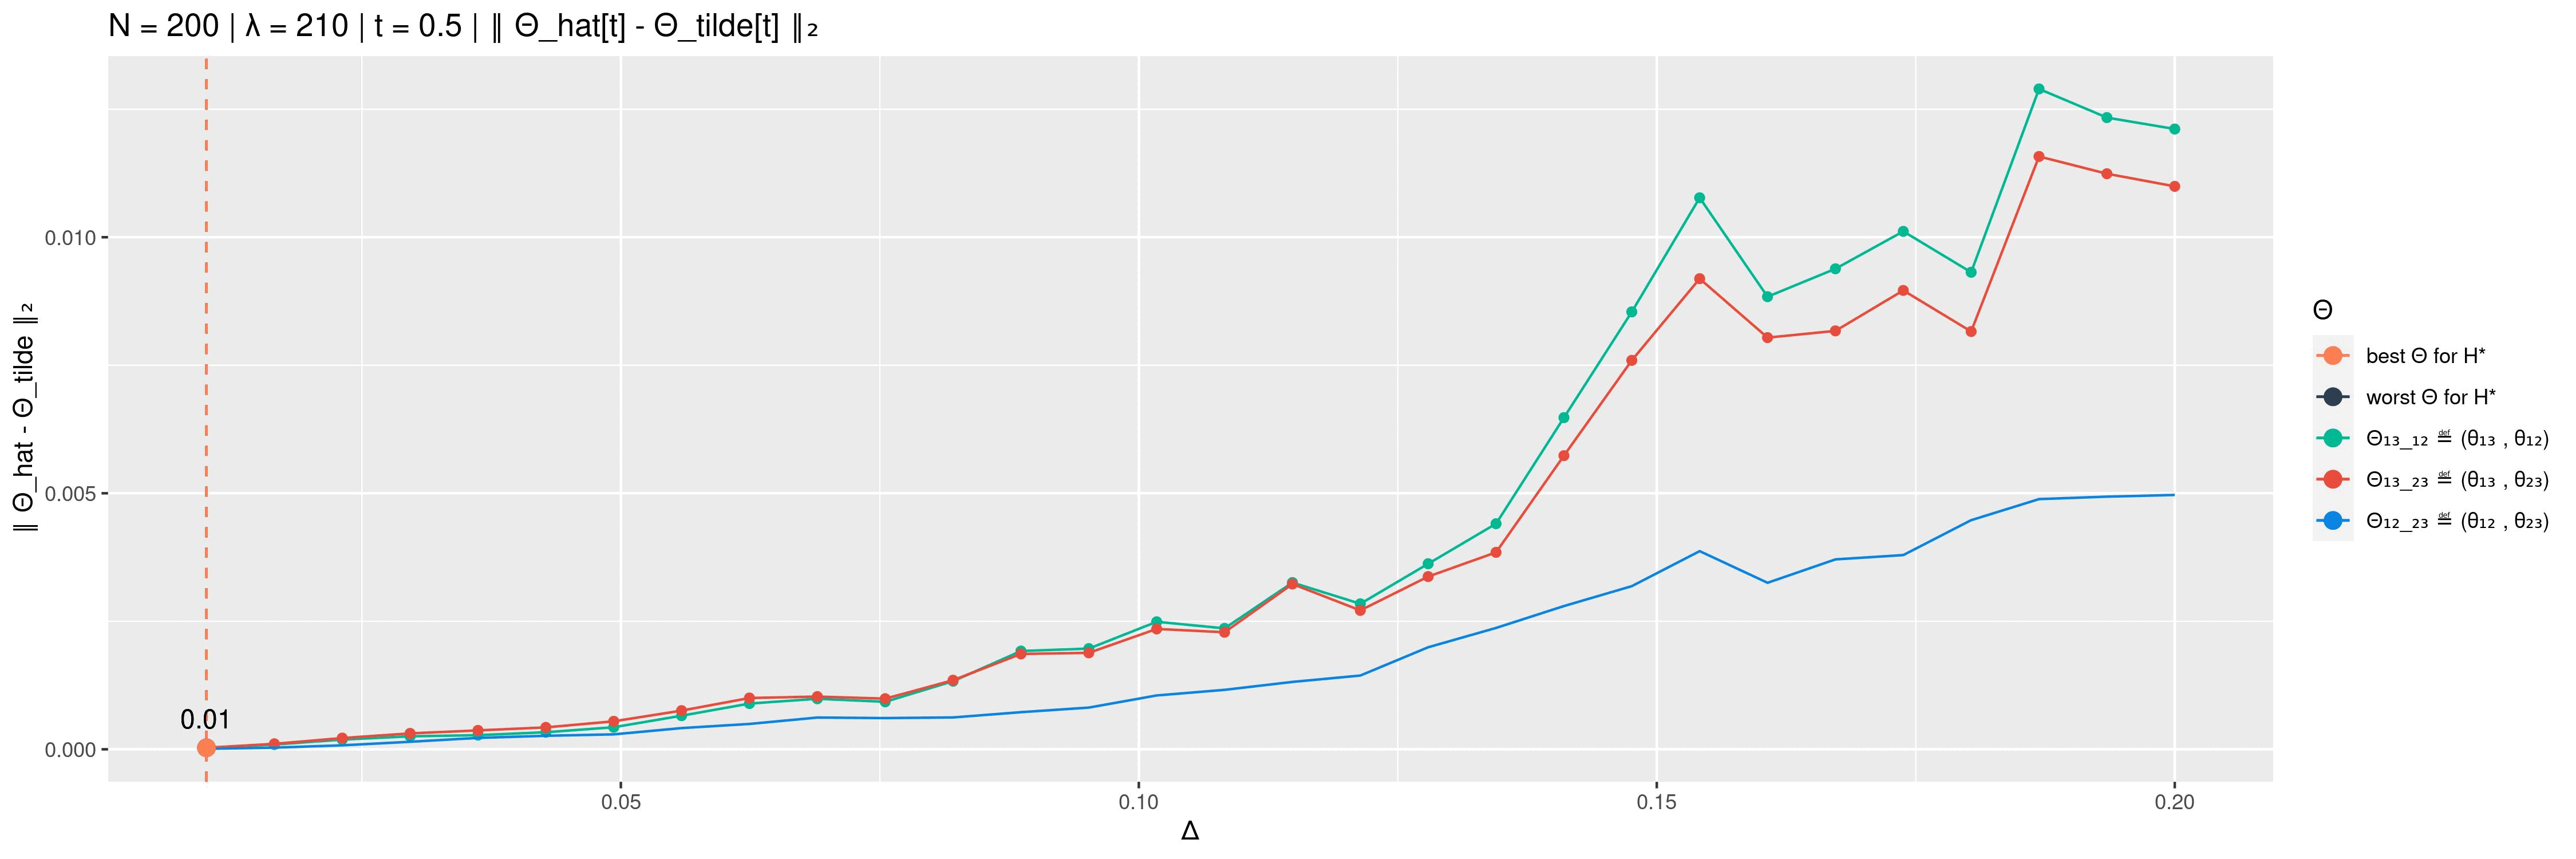
\includegraphics[width=0.8\textwidth]{Images/risque/N200_t0.5_lbd210.jpg}
\end{figure}


\begin{figure}[H]
	\centering
	\textbf{ H = 0.73 }

	Sparse :

	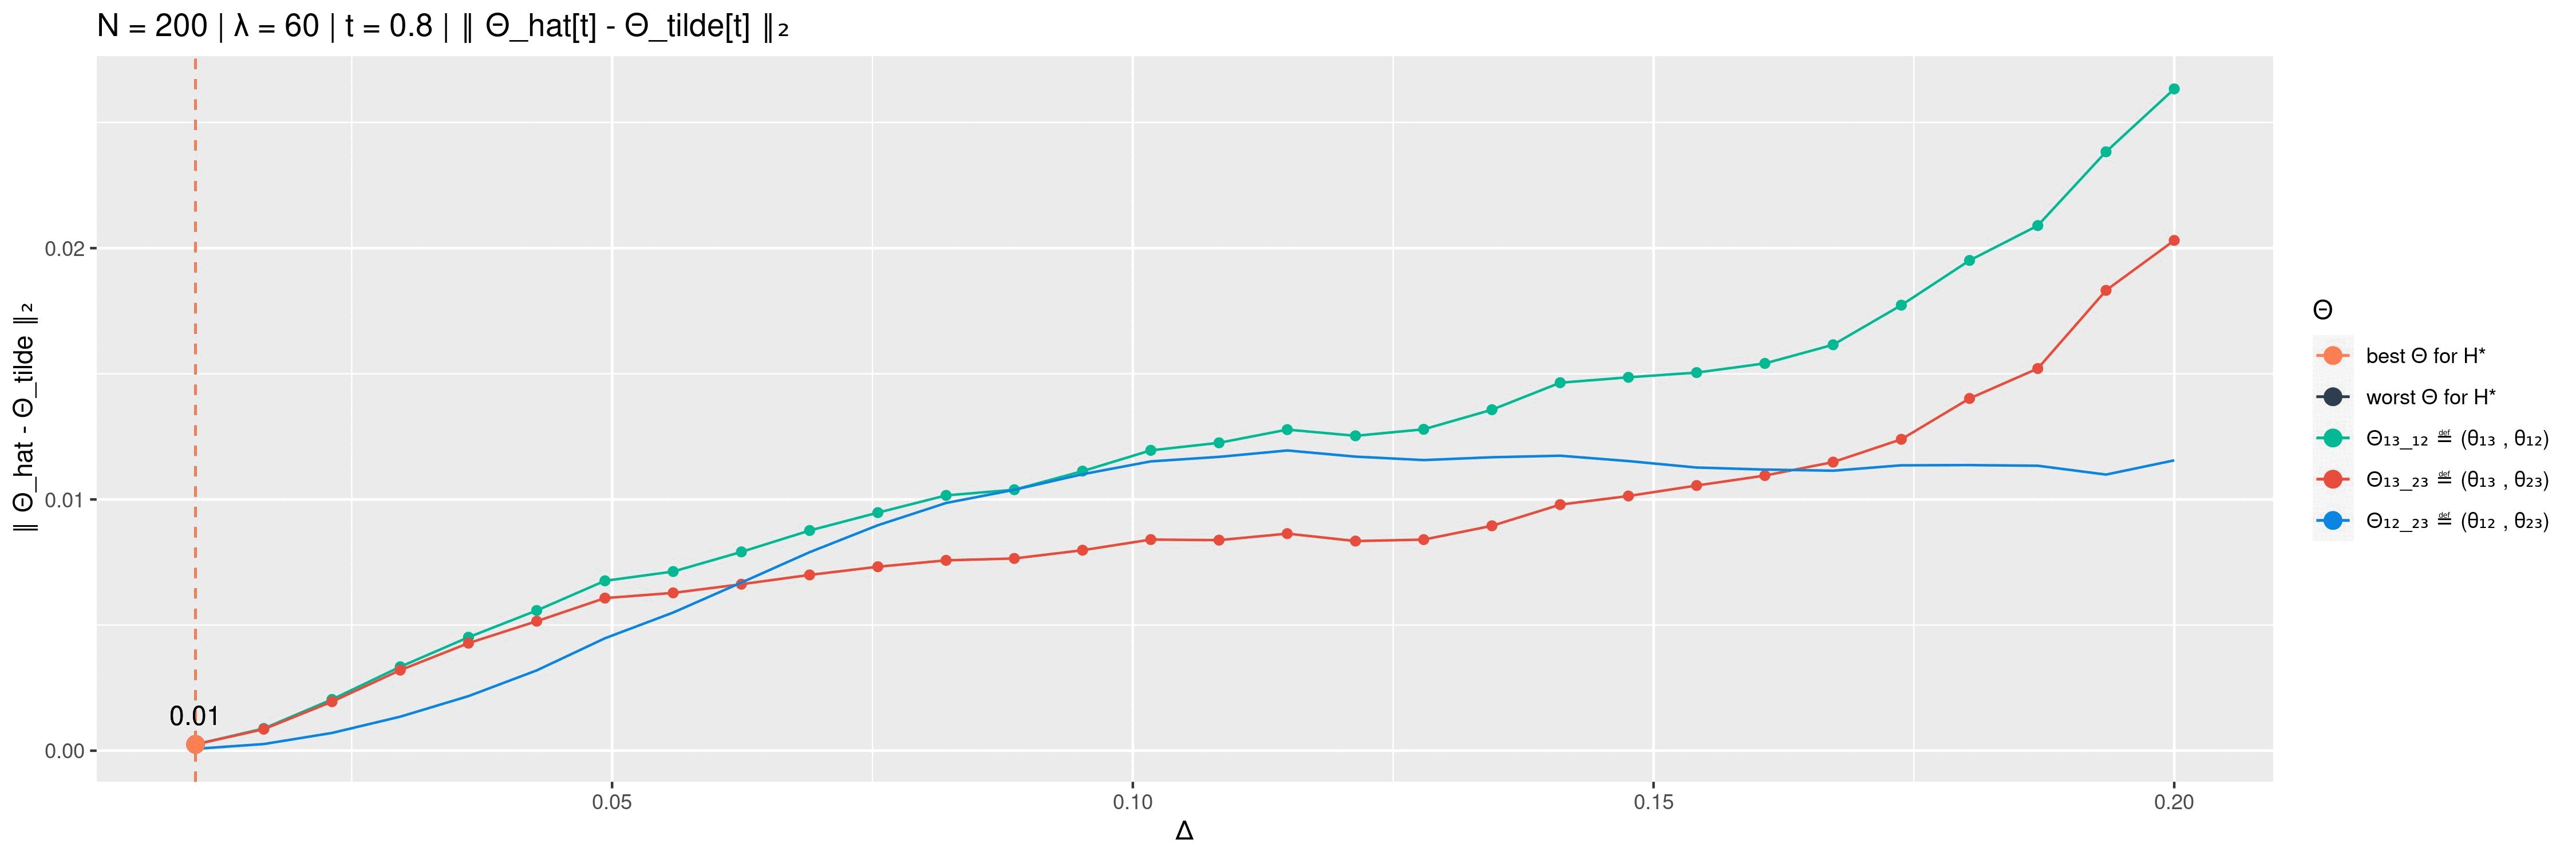
\includegraphics[width=0.8\textwidth]{Images/risque/N200_t0.8_lbd60.jpg}

	Dense :

	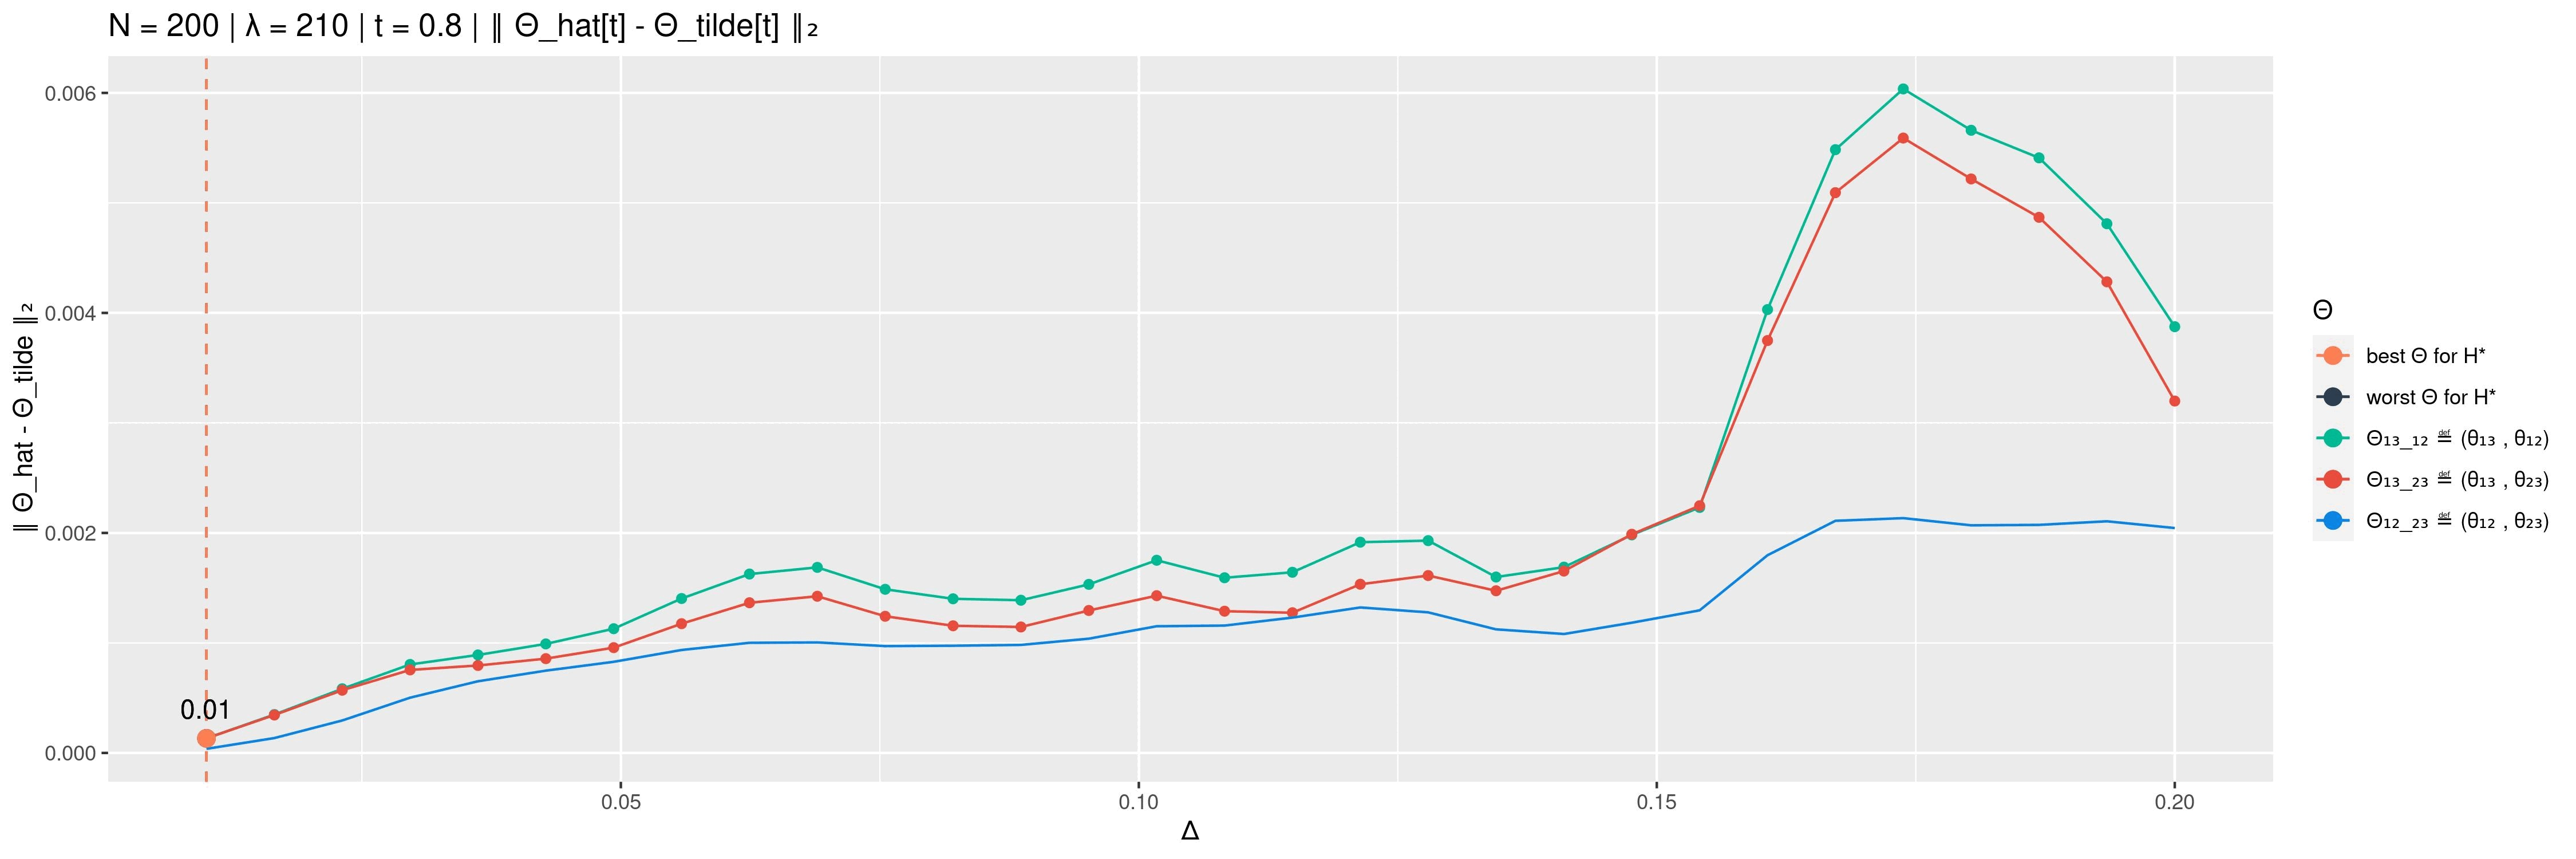
\includegraphics[width=0.8\textwidth]{Images/risque/N200_t0.8_lbd210.jpg}

	\label{fig:sparse_osef}
	\caption{Graphe des risques \textbf{euclidiens} dans les cas \og sparse \fg et \og raisonnablement dense \fg, ayant enlevé les observations extrêmes ($\leq$ 20\% des échantillons de monte carlo)}
\end{figure}


%%%%		RELATIF 		%%%%

\begin{figure}[H]
	\centering
	\textbf{ H = 0.51 }

	Sparse :

\includegraphics[width=0.8\textwidth]{Images/eucl_rel/N200_λ060_t0.3_kernel.jpg}

	Dense :

\includegraphics[width=0.8\textwidth]{Images/eucl_rel/N200_λ210_t0.3_kernel.jpg}
\end{figure}

\begin{figure}[H]
	\centering
	\textbf{ H = 0.6 }

	Sparse :

\includegraphics[width=0.8\textwidth]{Images/eucl_rel/N200_λ060_t0.5_kernel.jpg}

	Dense :

\includegraphics[width=0.8\textwidth]{Images/eucl_rel/N200_λ210_t0.5_kernel.jpg}
\end{figure}

\begin{figure}[H]
	\centering
	\textbf{ H = 0.73 }

	Sparse :

\includegraphics[width=0.8\textwidth]{Images/eucl_rel/N200_λ060_t0.8_kernel.jpg}

	Dense :

\includegraphics[width=0.8\textwidth]{Images/eucl_rel/N200_λ210_t0.8_kernel.jpg}

	\label{fig:sparse_osef_rel}
\caption{Graphe des \textbf{risques euclidiens relatifs} à $\widetilde \Theta(\Delta)$ dans les cas \og sparse \fg et \og raisonnablement dense \fg, ayant enlevé les observations extrêmes ($\leq$ 20\% des échantillons de monte carlo)}
\end{figure}


\section{Etude de l'impact de la méthode de prélissage sur l'estimation de la régularité et le $\Delta$ optimal}
\label{annexe:prelissage_impact}
On peut aussi se poser la question suivante, traîtée ici en annexe pour ne pas flouter la mission principale de ce stage :

\question{
	$\circled 4$ : La méthode de pré-lissage utilisée possède-t-elle un impact important sur l'estimation de la régularité et donc sur la stratégie de sélection du $\Delta$ en pratique ?
}

\question{Peut on quantifier le biais introduit par le lissage en utilisant les ondelettes sur l'estimation de la régularité locale ?}

\editlater{regarder ce que ça donne, en utilisant les différents théorèmes et bornes disponibles sur les ondelettes pour un processus Holder LORSQUE J AI LE TEMPS - certainement en Septembre}

\subsubsection{Pré-lissage Spline}

Le lissage spline est certainement une des méthodes de lissage les plus répandues de par sa simplicité d'implémentation. De plus la détermination des hyper-paramètres de lissage via la méthode de GCV permet de déterminer une approximation de base optimale à un coût computationnel relativement faible. Un des plus grands avantages du lissage B-Spline est l'obtention d'une base de fonctions, qui permet à coût de stockage faible de pouvoir prédire des points non observés. Une fois la base déterminée, il ne reste plus qu'à prédire les points non observés en utilisant la base de fonctions et les coefficients de la décomposition de la courbe sur cette base.

\bigskip

On rappelle que l'utilisation de Splines comme méthode de lissage nécessite tout de même de faire des choix : elle est sensible aux nombre de noeuds et leur emplacement. Il est donc nécessaire de les déterminer par validation croisée. Une méthode fréquemment utilisée est d'utiliser un nombre de noeuds $\mathcal k$ égal au nombre d'observations, et de les placer aux points d'observations. Puis on utilise des splines pénalisées sur leur dérivée seconde ( $L = L_{quad} + \lambda \displaystyle\int_0^1 f''(u) du$ ) et on détermine le paramètre de pénalisation par validation croisée afin de s'affranchir du choix du nombre de noeuds et de leur emplacement. La validation croisée sur la pénalisation est supposée compenser ce choix. Il s'agit de la méthode qui a été utilisée dans le cadre de ce stage, car très populaire et simple à mettre en place.

Il est à noter qu'une autre méthode de lissage spline est de déterminer le nombre de noeuds $k$ par validation croisée, et de placer les points de façon uniforme sur les quantiles de la distribution des observations. Ce qui ne sera pas utilisé dans le cadre de ce stage.

\bigskip

En effectuant un pré-lissage de splines cubiques naturelles sur une courbe Höldérienne, on ne s'attend pas à obtenir de bonnes performances sur l'estimation de la régularité locale. En effet les courbes splines sont par construction de classe $\mathcal C^2$ (fonctions polynômiales $\mathcal C ^\infty$ avec des raccordements $\mathcal C^2$), et la courbe lissée écrasera complétement l'information de régularité. Même si il s'agit de ce que l'on souhaite obtenir et qu'on ne connait pas encore la régularité, il est raisonnable de penser qu'être précautionneux dans le choix de la technique de lissage de telle façon à être le plus proche de la régularité d'une fonction qui pourrait potentiellement ne même pas être dérivable est une bonne idée.



\subsubsection{Pré-lissage à noyaux}

Considérer un lissage non paramétrique à noyaux est une alternative au lissage spline. L'espoir est la détermination lors du pré-lissage d'utiliser une fenêtre de lissage qui permette de mieux conserver l'information irrégulière que les splines via la détermination du $h^{*[\textsf{cv}]}_{\textsf{pre}}$ optimal par validation croisée.

\bigskip

Pour rappel, la fenêtre de lissage retenue est une fenêtre de lissage déterminée par validation croisée, qui est un estimateur de la fenêtre de lissage optimale pour le risque quadratique qui peut s'exprimer en fonction de la régularité locale si l'on suppose les hypothèses retenues sur le processus par MPV \cite{maissoro-SmoothnessFTSweakDep}. Même si le $h^*_{\mathcal R_{quadr}}$ est techniquement une fonction de $t \in \mathcal T$, l'estimateur que l'on considère lui sera sélectionné pour l'ensemble du support de la courbe $\mathcal T$. On peut espérer que si la courbe change de régularité sur son support mais que celui-ci ne varie pas trop, alors la fenêtre de lissage sélectionnée sera adaptée à la régularité locale de la courbe peu importe où l'on se trouve sur le support.


\subsubsection{Lisser en utilisant une base de fonction sans écraser l'information irrégulière ?}

Le lissage spline donne une fonction de classe $\mathcal C^2$, ce qui est un désavantage dans le cadre du prélissage qui sert à déterminer les paramètres de régularité de courbes issues d'un processus que l'on ne suppose pas plus régulier que continu. Toutefois, le fait d'utiliser une base de fonctions pour effectuer le lissage a de nombreux avantages par rapport au lissage à noyaux qui peuvent éventuellement s'avérer utiles dans certaines situations spécifiques pour la mise en production de modèles.

En effet, une fois que l'on a déterminé les composantes de la décomposition de notre signal sur la base de fonctions, on n'a plus besoin de se référer aux données pour prédire une valeur. Il s'agit d'une méthode très économe en mémoire, ce qui peut être très avantageux dans le cadre de la mise en production de modèles lorsqu'il y a de nombreuses courbes observées.



Le lissage spline donne une fonction de classe $\mathcal C^2$, ce qui est un désavantage dans le cadre du prélissage qui sert à déterminer les paramètres de régularité de courbes issues d'un processus que l'on ne suppose pas plus régulier que continu. Toutefois, le fait d'utiliser une base de fonctions pour effectuer le lissage a de nombreux avantages par rapport au lissage à noyaux qui peuvent éventuellement s'avérer utiles dans certaines situations spécifiques pour la mise en production de modèles.

En effet, une fois que l'on a déterminé les composantes de la décomposition de notre signal sur la base de fonctions, on n'a plus besoin de se référer aux données pour prédire une valeur. Il s'agit d'une méthode très économe en mémoire, ce qui peut être très avantageux dans le cadre de la mise en production de modèles lorsqu'il y a de nombreuses courbes observées.

\section{Ondelettes}
\subsection{Une brève introduction aux ondelettes}


Les ondelettes proviennent du monde du traîtement du signal. Elles répondent à un problème de représentation des données à la fois dans le domaine temporel et dans le domaine fréquentiel. En effet, la transformée de Fourier nous donne accès aux fréquences présentes dans un signal mais ne nous permet pas de localiser à quel moment sont intervenues les fréquences spécifiques. Le théorème d'indétermination de Heisenberg stipule que l'on ne peut avoir une résolution parfaite à la fois dans le domaine fréquentiel et le domaine temporel, il y a un compromis qui doit être fait. La question devient alors :

\question{
	\smallskip\centering
	Comment représenter une fonction dans le domaine temporel et dans le domaine fréquentiel de façon optimale ? En d'autres termes, quelle résolution temporelle et quelle résolution fréquentielle choisir ?
}

Une première approche proposée en 1946 par Denis Gabor est la transformée de Fourier à court terme (STFT). Celle-ci consiste à regarder la transformée de Fourier d'une fonction sur une fenêtre de taille fixe et à faire glisser cette fenêtre sur la fonction. On obtient ainsi la représentation fréquentielle de la fonction sur un intervalle de temps centré en un point que l'on peut faire varier.

\bigskip

\begin{minipage}{0.32 \textwidth}
	\begin{figure}[H]
		\centering
		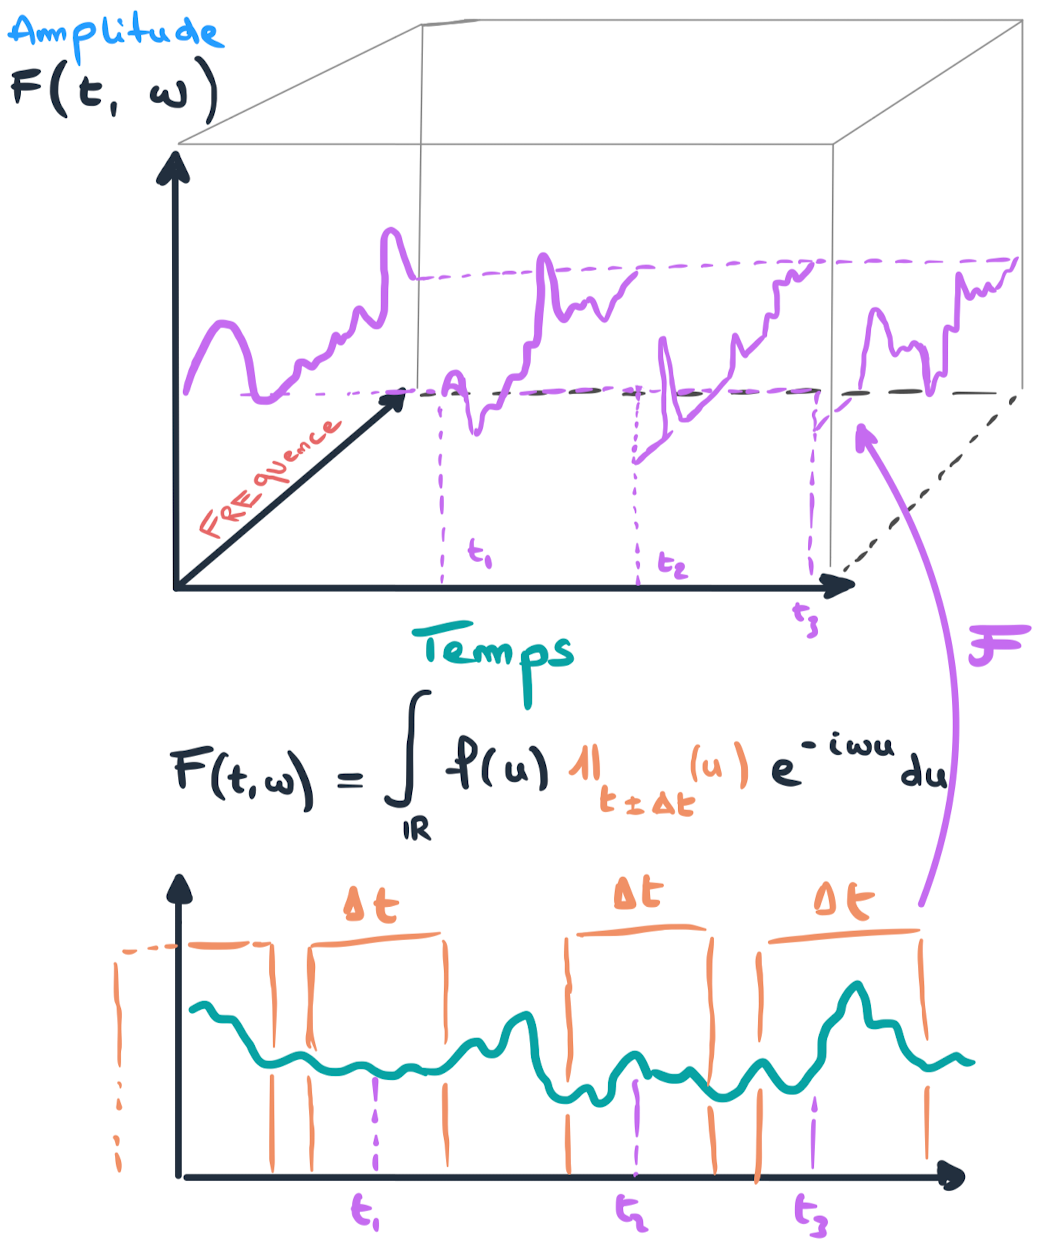
\includegraphics[width=\textwidth]{images/sketches/STFT.png}
		\caption{Transformée de Fourier à court terme d'une fonction}
		\label{fig:STFT}
	\end{figure}
\end{minipage}
\hfill
\begin{minipage}{0.60 \textwidth}

	Cependant contrairement à ce que peut suggérer le dessin présenté ici, la résolution fréquentielle n'est pas parfaite. Elle est d'ailleurs dans le cadre de la Transformée de Fourier à court terme constante, que ce soit sur le domaine temporel ou le domaine fréquentiel. La résolution fréquentielle est donc constante quelque soit la fréquence considérée.

	\question{
		\smallskip\centering
		Quel est le problème avec cette approche ?
	}

	le problème ne vient pas du monde mathématique mais plutôt du monde réel : les signaux que l'on observent présentent la caractéristique suivante : Les signaux de basse fréquence ont tendance à s'étendre sur la durée, et les signaux de hautes fréquences ont tendance à être très localisées, sous forme d'impulsion. Il devient alors clair que pour correctement identifier et localiser les fréquences présentes dans un signal, il est judicieux (voire parfois nécessaire) de varier la résolution fréquentielle et temporaire (limitées par le théorème d'indétermination de Heisenberg) en fonction de ce qui est le plus difficile à distinguer. C'est ce que proposent les ondelettes.

\end{minipage}


\subsection{Motivation dans le cadre de l'analyse de données fonctionnelles}

La capacité de capturer de façon efficiente les irrégularités\footnote{on pourra se référer pour la justification technique de cette affirmation l'annexe \ref{annexe:wavelet}} de la fonction lissée est une motivation pour l'utilisation de la base d'ondelettes pour effectuer le pré-lissage de données, dont on espère qu'il n'écrase pas la majorité de l'information irrégulière de nos données. Si une des méthodes possibles, comme mentionnée précédemment, est d'utiliser un lissage non paramétrique à noyaux, les bases de fonctions ont de nombreux avantages. Un des avantage est le fait qu'une fois les projections sur la base déterminées, il n'y a plus besoin de se référer de nouveau aux données originales par la suite. Cela donne une représentation très parcimonieuse des données. Alors pour déterminer la valeur de $\widehat X(t)$ en un point $t$ non observé, il suffit d'évaluer l'expression $\sum_k \prodscal X {\psi_k} \psi_k(t)$ avec $(\psi_k)_{k \in \llbracket 1, K \rrbracket}$ la base d'ondelettes tronquée déterminée par validation croisée.



% ! ——————————————————————————————————————————— !

\chapter{Un peu d'Histoire}
\label{annexe:histoire}
\section{ Histoire des séries temporelles }
% \book{ \textbf{Un peu d'histoire sur les séries temporelles \ldots}        
\info{une grande partie des informations présentées dans cette section histoire provient de la référience ~\cite{time_series_brief_history} }


\smallskip

Parmi les étapes importantes du développement des séries temporelles, on peut noter l'article \emph{Time Series Analysis : Forecasting and Control} de Box et Jenkins (1970) qui introduit le modèle ARIMA et une approche aujourd'hui standarde d'évaluation du modèle à utiliser ainsi que son estimation. Ce développement est dû en grande partie à l'utilisation de telles données dans les secteurs économiques et des affaires afin de suivre l'évolution et la dynamique de différentes métriques

\smallskip

L'étude des séries temporelle a été divisée en l'étude du domaine fréquentiel, qui étudie le spectre des processus pour le décomposer en signaux principaux, et du domaine temporel, qui étudie les dépendances des indices temporels. L'utilisation de chacune des approches était sujet à débats mouvementés jusqu'aux alentours de l'an $2000$.

\smallskip

Le développement des capacités de calcul a été une révolution notamment pour l'identification des modèles (le critère AIC, l'estimation par vraissemblance dans les années $1980$, \ldots).
% modèles à espace d'états et le filtre de Kalman pour évaluer cette vraissemblance efficacement, MCMC, \ldots).

\smallskip

À partir des années $1980$, les modèles non linéaires émergent (ARCH par Engle, modèles à seuil \ldots) et trouvent application en économie notamment. Enfin l'étude multivariée (modèle VAR) fait surface dans les années 1980 par Christopher Sims~\cite[ \href{https://pubs.aeaweb.org/doi/pdf/10.1257/jep.15.4.101}{lien de l'article} ]{VAR_paper}

\smallskip

Une large partie de la théorie s'appuie notamment sur l'étude des racines de l'unité, en considérant un polynôme d'opérateur $P(B) = (I + \sum_k a_k B^k)$ à partir duquel les relations d'autocorrélations peuvent se ré-écrire.
% }
\pagebreak
\section{ Histoire des données fonctionnelles }
% \book{ \textbf{\ldots et un peu d'histoire sur les données fonctionnelles}
\info{Pour une description plus complète de l'histoire du développement de l'analyse fonctionnelle, on pourra se référer à \href{https://anson.ucdavis.edu/~mueller/fdarev1.pdf}{\textcolor{flatuicolors_blue_deep}{cet article de Wang, Chiou et Müller}}~\cite{wang2016functional}}


Bien que l'histoire du développement de l'Analyse de Données Fonctionnelles (FDA) puisse être retracée jusqu'aux travaux de Grenander et Karhunen~\cite{karhunen1946spektraltheorie} dans les années 1940 et 1950, où l'outil a été utilisé pour étudier les courbes de croissance en biométrie, ce sous-domaine de la statistique a été étudié de manière systématique à partir des années 1980.

\bigskip

En effet, c'est J.O. Ramsay qui a introduit l'appellation de "données fonctionnelles" en 1982~\cite{ramsay1982data} et qui contribuera en partie à sa popularisation. La thèse de Dauxois et Pousse en 1976 sur l'analyse factorielle dans le cadre des données fonctionnelles\cite{dauxois1976analyses} a ouvert la voie à l'analyse par composante principale fonctionnelle (FPCA), un outil clé pour l'étude des données fonctionnelles. La FPCA permet d'étudier des objets fonctionnels qui sont de dimension infinie, difficiles à manipuler et impossibles à observer empiriquement, en dimension finie et surtout sur $\R d$ que l'on connait bien.

\bigskip

Au cours des années 2000, de nombreux outils statistiques déjà développés pour des données à valeurs dans $\R d$ depuis un siècle, tels que la régression linéaire (éventuellement généralisée), les séries temporelles ou encore les modèles additifs, ont été adaptés aux données fonctionnelles.
Par exemple, les modèles de régression linéaire fonctionnelle ont été développés avec une réponse fonctionnelle~\cite{ramsay1991some} ou scalaire~\cite{cardot1999functional} en 1999.
Les modèles linéaires généralisés ont également été étudiés~\cite{james2002generalized,muller2005generalized}, avec l'estimation de la fonction de lien par méthode non paramétrique à direction révélatrice \emph{(Single Index Model)} récemment étudiée en 2011~\cite{chen2011single}.
Cette méthode avait déjà été utilisée en économétrie pour des données de $\R d$ depuis 1963~\cite{sharpe1963simplified}, et leur estimation directe a été étudiée une décennie auparavant par M.Hristache, Juditsky et Spokoiny~\cite{hristache2001direct}. De même, les modèles additifs ont été étendus aux données fonctionnelles en 1999 par Lin et Zhang~\cite{lin1999inference}.
Enfin, le livre de Bosq, \emph{\textcolor{flatuicolors_blue_devil}{Linear Processes in Function Spaces : Theory and Applications}}~\cite{bosq2000linear}, publié en 2000, a contribué au développement des séries temporelles pour les données fonctionnelles.

\bigskip

Depuis lors, des ressources telles que l'ouvrage de Kokoszka et Reimherr, \emph{\textcolor{flatuicolors_blue_devil}{Introduction to Functional Data Analysis (2017)}}~\cite{kokoszka2017introduction}, rendent la théorie et la mise en production des méthodes d'analyse et de prédiction de données fonctionnelles plus accessibles.
% }

\pagebreak
\section{Histoire du mouvement brownien et de ses applications}
\input{content/annexe/histoire/histoire_brownien.tex}
\pagebreak

% ! ——————————————————————————————————————————— !

\chapter{Algorithmes \& Implémentations}

\label{annexe:code}
\section{Algorithmes de simulation}

\begin{algorithm}[H]
	\caption{$\operatorname{Get\_single\_mc\_sim}$ : Génération de FAR pour chaque valeur sur la grille}\label{alg:gen_far_grid}
	\KwData{

	}
	\KwIn{
		$\vec t$ : endroits où évaluer la régularité

		Régularité de $X_n$ sur $[0,1]$ : $H : t \mapsto H_t$

		fonction moyenne : $\mu$
	}
	\KwOut{$L = \left\{ L[N, \lambda] : N \in \overrightarrow N, \lambda \in \lbdset   , n \in \nset \right\}$}
	\KwResult{$\simsetall$}


	\Comment*[l]{** ———— Paramètres utilisés ———— **}
	$G \gets 100$
	\Comment*[l]{Grille d'approximation de l'$\int$}\;


	$B \gets 100$
	\Comment*[l]{Burn-in de la relation FAR(1)}\;

	$\overrightarrow \Delta \gets \begin{bmatrix} 0.01 & \dots & 0.2\end{bmatrix}_{30}$
	\Comment*[l]{diamètre du voisinage $J_\Delta$}\;

	$\overrightarrow N \gets \begin{bmatrix} 100 & 200 & 300 & 400\end{bmatrix}_4$
	\Comment*[l]{nombre de courbes}\;

	$\mathbf \Lambda \gets \begin{bmatrix} 30 & 45 & \dots & 480 \end{bmatrix}$
	\Comment*[l]{nombre moyen de points observés sur une courbe}\;

	\Comment*[l]{** ———————————————————————————— **}

	$L = [ \quad ]$\;

	\For{$N \in \overrightarrow N$}{
	\Comment*[f]{$\overrightarrow N = [100, 200, 300, 400]$}

	\For{$\lambda \in \mathbf \Lambda$}{
		%{$\lambda\gets30$ \KwTo $480$ \KwBy $15$}{

		$\genxset \gets \operatorname{far\_sim}(N, \lambda, H, \mu, B, G, \vec t, \overrightarrow \Delta)$ \; \Comment*[f]{génération}

	}

	$L[N, \lambda] \gets \genxset$
	}

	\Return{$L$}
\end{algorithm}

\begin{algorithm}[H]
	\caption{Simulation de Monte Carlo}\label{alg:gen_far_mc}

	\For{ $\textsf{mc} \gets 1$ \KwTo $200$ }{
		$L_\textsf{mc} \gets \operatorname{Get\_single\_mc\_sim}(H, \mu)$
	}

	\Return{$\left\{ L_{\textsf{mc}} : \textsf{mc} \in \llbracket 1, 200 \rrbracket \right\}$}

\end{algorithm}

\begin{algorithm}[H]
	\caption{$\operatorname{far\_sim}$ : Simulation d'un $\operatorname{FAR}(1)$}\label{alg:far_sim}
	\KwIn{
	$N \in \mathds N^*$ : nb $X_n$

	$\lambda \in \mathds N^*$ : nb moy pts observés

	$H : t \mapsto H_t$ : régularité

	$\mu : [0,1] \rightarrow \mathds R$ : moyenne

	$B \in \mathds N^*$ : Burn-in du FAR(1)

	$G \in \mathds N^*$ : grille méthode des rectangles

	$\overrightarrow \Delta$ : tous les diamètres testés

	$\vec t$ : endroits où évaluer la régularité
	}
	\BlankLine
	\KwResult{
		$\simset$

		avec $X_{n+1}(t) = \int \beta(u,t)X_n(t) + \eta_{n+1}$
	}

	\BlankLine
	\midrule
	\BlankLine
	$N_t \gets \operatorname{len}(\vec t)$\;
	$N_{calc} \gets N + B$
	\BlankLine

	\Comment*[l]{points de comparaison avec le lissage}
	$T(\Delta) = \begin{bmatrix} t_1[1] = \vec t[1] - \frac \Delta 2 & t_2[1] = \vec t[1] & t_3[1] = \vec t[1] + \frac \Delta 2 \\ \vdots & \vdots & \vdots \\  t_1[N_t] = \vec t[N_t] - \frac \Delta 2 & t_2[N_t] = \vec t[N_t] & t_3[N_t] = \vec t[N_t] + \frac \Delta 2 \end{bmatrix}$\;

	\BlankLine
	\Comment*[l]{Points observés}
	$T_{obs}\gets \mathcal U( [0,1] )^{\otimes \lambda}$\;

	\BlankLine
	\Comment*[l]{Grille de la méthode des rectangles médians}
	$\textsf{grid}_{\int} \gets \left( \frac{(k-1) + (k)}{2} \right)_{k \in \llbracket 1, G \rrbracket}$\;

	\BlankLine
	\Comment*[l]{Ensemble des points}
	$T \gets T_{obs}\bigcup T(\Delta) \bigcup \textsf{grid}_{\int}$\;

	$T \gets \operatorname{order}(T)$\;


	\BlankLine
	\BlankLine
	\Comment*[l]{Simulation de mouvement brownien multi fractionnaire de régularité $(H,L)$}
	$L = [ \quad ]$\;

	\For{$k \in \llbracket1 , N_{calc} \rrbracket$}{
		$\varepsilon_k \gets \operatorname{mfBm\_sim}(T, H, L)$\;

		$\mu_k \gets \mu(T)$\;

		$L[k] \gets \begin{bmatrix} T, \varepsilon_k, \mu_k \end{bmatrix}$\Comment*[f]{$\in \mathcal M_{\operatorname{len}T, 3}(\mathds R)$}\;
	}

	\BlankLine
	\BlankLine
	\Comment*[l]{Simulation de la relation FAR(1)}
	\Comment*[l]{$X_{n+1}(t) = \mu(t) + \displaystyle\int_0^1 \beta(u, t)X_n(u) du + \varepsilon_{n+1}$}
	\For{$k \in \llbracket1 , N_{calc} \rrbracket$}{
		$K_\beta = \begin{bmatrix} \ddots & \vdots & \rddots \\ \dots & \beta(s,t) & \dots \\ \rddots & \vdots & \ddots  \end{bmatrix}$\;
		$I(\beta, \mathds X_{k-1}) = \frac 1 G  K_\beta \mathds X_{k-1}$\;
		$\mathds X_k \gets \mu_k + I(\beta, \mathds X_{k-1}) + \varepsilon_k$\;
	}

	\Return{ $(\mathds X_n)_{n \in \llbracket B+1, N_{calc} \rrbracket}$ }
\end{algorithm}

%\pagebreak
%\section{Implémentation R}
%\label{annexe:code-R}
%\ifnum\value{code}=1
	\subsection{packages utilisés}
	\begin{minted}[linenos=true, mathescape=true, frame=single, breaklines]{R}
    # ——— install ——— #
    install.packages(c("data.table","wavethresh","fda", "fda.usc"))
    # ——— general packages ——— #
    library(data.table)
    # ——— FDA packages ——— #
    library(fda)
    library(fda.usc)
    # ——— Wavelet packages ——— #
    library(wavethresh)
\end{minted}

\subsection{Simulation des FAR}

\subsubsection{code d'une simulation de monte-carlo}

\begin{minted}[linenos=true, mathescape=false, frame=single, breaklines]{R}
simulation_far_lambda_mc <- far.sim(
    N = N,
    lambda = lambda,
    distribution = runif, 
    hurst = chosen_hurst, 
    kernel = autoregressive_kernel,
    L = 1,
    mu = mu_simul,
    burnin = 100,
    remove_burnin = TRUE,
    G = 100,
    t_vector = seq(from = 0.3, to = 0.8, length.out = 6),
    delta_vector = seq(1e-2, 2e-1, length.out = 30),
    mc = mc_index
)
\end{minted}

\subsubsection{Points utilisés pour la simulation}

\begin{minted}[linenos=true, mathescape=false, frame=single, breaklines]{R}
# random design
points_list <- random_design(N = n, lambda = lambda, distribution = distribution)
# les points où on génère le mfBm
times <- c(points_list[[x]], grid, t_dt[, t1], t_dt[, t2], t_dt[, t3])
# identification des points : observé / grille integrale / comparaison lissage
fac <- as.factor(c(
    rep("observed", length(points_list[[x]])), rep("integral_grid", G),
    rep("t1", n_delta * m), rep("t2", n_delta * m), rep("t3", n_delta * m)
))
# identification de t1,t2,t3
t_index_fac <- as.factor(c(
    rep(NA, length(points_list[[x]])), rep(NA, G),
    rep(t_dt[, t_index], 3)
))
# quelle valeur de delta le t1,t3 correspondent
delta_index_fac <- as.factor(c(
    rep(NA, length(points_list[[x]])), rep(NA, G),
    rep(t_dt[, delta_index], 3)
))
# les points où on simule, identifiés :
df <- data.table(times = times, fac = fac, t_index = t_index_fac, delta_index = delta_index_fac)
\end{minted}

\subsubsection{Innovations : mfBm}

\begin{minted}[linenos=true, mathescape=false, frame=single, breaklines]{R}
X[[i]]$eps <- mfBm.sim(times[[i]]$times, hurst, L)
\end{minted}

\subsubsection{Relation FAR}

\begin{minted}[linenos=true, mathescape=false, frame=single, breaklines]{R}
X[[1]]$X <- X[[1]]$mu + X[[1]]$eps
for (i in 2:n) {
    times <- X[[i]]$times
    Xold <- X[[i - 1]]$X[X[[i - 1]]$fac == "integral_grid"] - X[[i - 1]]$mu[X[[i - 1]]$fac == "integral_grid"]
    Enew <- X[[i]]$eps
    tmp <- expand.grid(s = times, t = grid)
    s <- tmp$s
    t <- tmp$t
    beta <- matrix(kernel(s, t), ncol = G, byrow = FALSE)
    X[[i]]$X <- X[[i]]$mu + as.numeric((1 / G) * beta %*% matrix(Xold, ncol = 1) + Enew)
}
\end{minted}

\section{Lissage des courbes}


\begin{minted}[linenos=true, mathescape=false, frame=single, breaklines]{R}
...
\end{minted}



\section{Détermination de la régularité locale}

\begin{minted}[linenos=true, mathescape=true, frame=single, breaklines]{R}
get_reg_dt <- function(sm_dt) {
    sm_dt <- sm_dt[!(is.nan(xt1) | is.nan(xt2) | is.nan(xt3))]
    reg_dt <- rbindlist(
        lapply(
        split(sm_dt, by = c("delta_index", "t2")),
        function(dt) {
                # $\frac{1}{N}\sum_i \left[ \widehat{X}(v) - \widehat{X}(u) \right]^2$
                res <- dt[, lapply(.((xt1 - xt2)^2, (xt1 - xt3)^2, (xt3 - xt2)^2), mean)] 
                colnames(res) <- c("theta_12", "theta_13", "theta_23")
                res[, c("t", "delta_index", "delta") := .(dt[1, t2], dt[1, delta_index], dt[1, delta])]
                return(res)
            }
        )
    )
    # $\widehat{H_t} = \frac{\log \left( \widehat{\theta}(t_1, t_3) \right) - \log \left( \widehat{\theta}(t_1, t_2) \right)}{2 \log(2)}$
    reg_dt[, H := (log(theta_13) - log(theta_12)) / (2 * log(2))] 
    # $\widehat{L_t} = \frac{\widehat{\theta}(t_1, t_3)}{\Delta^{2 \widehat{H_t}}}$
    reg_dt[, L := theta_13 / (delta^(2 * H))] 
    return(reg_dt)
}
\end{minted}

\section{Détermination des risques}

\begin{minted}[linenos=true, mathescape=true, frame=single, breaklines]{R}
risk_eucl_dt <- function(N, lbd, sm_method) {
    base_path <- "/home/hbrunet/pfe-hugo-brunet/no_pkg/"
    reg_path <- "regularity/"       # régularité $\widehat{H_t}   | \widehat{\theta}(u,v) = \frac{1}{N} \sum_i (\widehat{X}_i(v) - \widehat{X}_i(u))^2$
    treg_path <- "regularity_true/" # régularité $\widetilde{H_t} | \widetilde{\theta}(u,v) = \frac{1}{N} \sum_i ( X_i(v) - X_i(u))^2 $

    for (m in 1:200) {
        reg_file <- glue::glue("reg_N{N}_lbd{lbd}_logistic_{sm_method}_mc{m}.rds")
        treg_file <- glue::glue("regtrue_N{N}_lbd{lbd}_logistic_{sm_method}_mc{m}.rds")

        rg <- readRDS(glue::glue(base_path, reg_path, reg_file))
        trg <- readRDS(glue::glue(base_path, treg_path, treg_file))

        rg_t <- split(rg, by = "t")
        trg_t <- split(trg, by = "t")

        w_mc <- rbindlist(lapply(names(rg_t), function(t_v) {
            u <- rg_t[[t_v]]
            v <- trg_t[[t_v]]

            e_12_13 <- (u[, theta_12] - v[, theta_12])^2 + (u[, theta_13] - v[, theta_13])^2
            e_13_23 <- (u[, theta_13] - v[, theta_13])^2 + (u[, theta_23] - v[, theta_23])^2
            e_12_23 <- (u[, theta_12] - v[, theta_12])^2 + (u[, theta_23] - v[, theta_23])^2

            data.table(
                t = u[, t],
                delta = u[, delta],
                eucl_12_13 = e_12_13,
                eucl_13_23 = e_13_23,
                eucl_12_23 = e_12_23
            )
        }))
        w_mc[, mc := m]
        if (m == 1) {
                w <- w_mc
            } else {
                w <- rbind(w, w_mc)
                rm(w_mc)
            }
    }
}

# Création des tables de risques avec aggregation des multiples simulations de monte carlo :
r_dt_lbd <- readRDS(...) # table des risques calculées précédemment

#  $\theta_{12} : \theta(t_1, t_2)$ + $\theta_{13} = \theta(t_1, t_3)$

r_dt_12_13 <- r_dt_lbd[, .(
    mean(eucl_12_13), 
    median(eucl_12_13), 
    var(eucl_12_13), 
    mad(eucl_12_13), 
    quantile(eucl_12_13, 0.05), 
    quantile(eucl_12_13, 0.25), 
    quantile(eucl_12_13, 0.75), 
    quantile(eucl_12_13, 0.95)
    ), by = .(t, delta) ]
names(r_dt_12_13) <- c("t", "delta", "mean", "median", "var", "mad", "q_05", "q_25", "q_75", "q_95")

# ... similaire pour les autres couples
\end{minted}

\section{Lissage adaptatif}

Dans la subsection \ref{annexe:estim_adapt}, nous avons mentionné qu'il était judicieux de lisser les courbes de façon adaptative à la quantité que l'on souhaite estimer. Si l'on a mentionné le risque à minimiser pour chaque quantité que l'on souhaite estimer, aucun détail n'a été fourni car il alourdit considérablement la trame de l'objectif du stage sans apporter des informations cruciales.

\bigskip

Cependant pour l'implémentation d'un tel lissage adaptatif, il fallait évidemment se référer au détail de l'expression pour pouvoir évaluer ce risque et déterminer la meilleure fenêtre.

\bigskip

\begin{equation*}
    R_\mu( \, t \, , h \, ) =
    \underbracket[0.187ex]{L_t^2 h ^{2H_t} \mathds B( \, t, h, 2H_t \,) }_{\textsf{contrôle du biais}}
    + \underbracket[0.187ex]{\sigma^2 \mathds V_\mu( \, t, h \, ) }_{\textsf{contrôle de la variance}}
    + \underbracket[0.187ex]{\frac{\mathds D_\mu( \, t \, )}{P_N(t, h)}}_{\textsf{contrôle de la dépendance}}
\end{equation*}

Développons maintenant les différentes quantités présentes dans l'expression :

\begin{equation*}
    {\mathds D_\mu( \, t \, )} \isdef
\end{equation*}
\begin{equation*}
    \mathds V_\mu( \, t, h \, ) \isdef
\end{equation*}
\begin{equation*}
    \mathds B( \, t, h, 2H_t \,) \isdef
\end{equation*}
\begin{equation*}
    P_N(t, h) \isdef
\end{equation*}

Dont l'implémentation sous R est la suivante :

\begin{minted}[linenos=true, mathescape=false, frame=single, breaklines]{R}
...
\end{minted}
\fi


